\documentclass[nobib,justified]{tufte-latex-3.5.0/tufte-book}% use "amsart" instead of "article" for AMSLaTeX format
%\usepackage{geometry}                		% See geometry.pdf to learn the layout options. There are lots.
%\geometry{letterpaper}                   		% ... or a4paper or a5paper or ... 
%\geometry{landscape}                		% Activate for for rotated page geometry
%\usepackage[parfill]{parskip}    		% Activate to begin paragraphs with an empty line rather than an indent


\usepackage{appendix}
\usepackage{graphicx}				% Use pdf, png, jpg, or eps with pdflatex; use eps in DVI mode
\usepackage[plain]{fancyref}								% TeX will automatically convert eps --> pdf in pdflate
\usepackage{amsmath}
\usepackage{mathtools}	
\usepackage{amssymb}
\usepackage{amsthm}
\usepackage{hyperref}
%\usepackage[bitstream-charter]{mathdesign}
\usepackage{epigraph}
\usepackage{xspace}
%\usepackage{marginfix}


%\usepackage[backref=true,natbib=false,backend=bibtex,autocite=footnote]{biblatex}
\usepackage[backend=bibtex,style=numeric,sorting=none]{biblatex}
\renewcommand\nameyeardelim{, }

\addbibresource{library.bib}

%\newcommand*{\fancyrefthmlabelprefix}{eq}
\newcommand*{\fancyrefthmlabelprefix}{thm}
\frefformat{plain}{\fancyrefthmlabelprefix}{theorem~#1}
\Frefformat{plain}{\fancyrefthmlabelprefix}{Theorem~#1}
\newcommand*{\fancyrefapplabelprefix}{app}
\frefformat{plain}{\fancyrefapplabelprefix}{appendix~#1}
\Frefformat{plain}{\fancyrefapplabelprefix}{Appendix~#1}
\newcommand{\pd}[2]{\frac{\partial #1}{\partial #2}}
\DeclareMathOperator{\argmin}{argmin}
\DeclareMathOperator{\Tr}{Tr}
\DeclareMathOperator{\Diag}{Diag}
\DeclareMathOperator{\argmax}{\arg\max}
\DeclareMathOperator{\cotan}{cotan}
\newcommand{\mycite}{\autocite}
\newcommand{\mycitep}{\parencite}
\newcommand{\mycitet}{\textcite}

\newcommand{\covar}{E}

\newsavebox{\titleimage}
\savebox{\titleimage}{\includegraphics[width=20\baselineskip]{figures/wordcloud.png}}

\title[Optimal Population Coding of Dynamic Stimuli]{\setlength{\parindent}{0pt}Optimal Population\\
Coding of\\
Dynamic Stimuli\\
\vspace{2cm}
\usebox{\titleimage}}
\author{Alex Kunze Susemihl}
\date{Summer 2014}							% Activate to display a given date or no date

\begin{document}
%\morefloats
\maketitle
\setcounter{tocdepth}{2}
\setcounter{secnumdepth}{1}
\tableofcontents
\chapter{Introduction}

\label{chap:intro}

\newthought{Neuroscience as a whole} is concerned with the function of the nervous system. More precisely, it asks a very simple question: {\em What is the brain 
doing?}\footnote{ Or alternatively: {\em What is the nervous system doing?}} The simplicity with which humans and animals perform in their environment makes it 
almost unnatural to ask how their brains enable these behaviors. It is often hard to explain to laymen the complexity involved in preparing even the simplest actions, 
such as saccades or walking, such is the ease with which these are normally performed. Although one can not realistically expect to answer that question in any 
general fashion, I will try to touch upon a number of points which shed light on some aspects of the nervous system and provide us with a {\em guiding principle} to 
understand what the brain is doing, why and possibly how.\par

Neuroscience was born as a branch of biology, and although it is now often thought of as  an interdisciplinary science in itself, its objects of study are still to the 
largest extent biological systems. Theodosius Dobzhansky published an influential essay in 1973, entitled {\em Nothing in biology makes sense except in the light of 
evolution},\cite{Dobzhansky1973} which defends exactly that point. Though it has been reviewed and revisited constantly since its proposal, the theory of evolution 
through natural selection remains the central pillar of biological sciences. As such, neuroscience must also view its objects of study through the lenses of evolution. 
More specifically, we can then ask ourselves {\em What evolutionary advantage would this brain bring to an individual?} instead of {\em Why is the brain this way?} 
That being said,  there are caveats in the case of neuroscience. For one, the brain is capable of plasticity and adaptation unthinkable for other organs, and so we can 
not expect to understand the functionality of the brain in the same way in which the shape of bird beaks can be understood as a function of their preferred fruits and 
seeds. Furthermore, the brain controls all of the motor and perceptual apparatus, having a multitude of uses and purposes, unlike simpler organs.\par

One particular aspect of the brain which has received increasing attention recently is its ability to deal with uncertainty. In a very fruitful line of research, a number 
of experiments have demonstrated that humans and animals integrate uncertain information in a near-optimal way. The so-called {\em Bayesian Brain},\cite{Knill2004} 
would explicitly represent the distribution over world states and perform inference in a manner consistent with Bayesian inference, obtaining optimal integration of 
sensory cues from different modalities, for example. It is still a matter of debate how these Bayesian computations would be implemented in the brain. One possibility 
is that the activity of neurons is sampling from a representation of the distribution of world states,\cite{Berkes2011} which is frequently called the {\em sampling 
hypothesis}. Another is that the activity of the neurons itself represents the likelihood over world states,\cite{Ma2006} and the population as a whole codes for the 
distribution, hence the term {\em population coding}.\par

\subsection*{Structure}

\newthought{The main goal of this thesis} is to develop a conceptual framework for studying optimal population coding in a dynamic framework. Furthermore, I will
establish a link between optimal dynamic encoders and the efficient coding hypothesis, first proposed by Horace Barlow.\cite{Barlow1961} I believe that the 
inclusion of time into the coding framework raises a number of questions, which have not been addressed in the scientific literature properly. In the remainder of this 
chapter, I will discuss the efficient coding hypothesis and its more recent developments, and I will touch upon its relationship to Shannon's information theory.\cite{Shannon1948} I will finish by discussing the issue of dynamic population coding, highlighting the issues which I believe are of importance in considering the 
temporal aspect of coding. I will make the case for a study of optimal filtering of partially observed stimuli as a model of stimulus inference based on spike trains. 
Following, in \fref{chap:filtering}  I will introduce the general theory of filtering of stochastic stimuli. After that, in \fref{chap:MSE} I will discuss results regarding the 
Mean-Squared-Error (MSE) of optimal filters of point process data, presenting a number of new analytical results. In \fref{chap:control}, I will generalize the filtering 
framework to control problems, showing results for optimal control theory of point process-observed processes. In \fref{chap:optimal} I will then provide the connection 
to neuroscience, by considering the optimal encoding strategy for a population of neurons coding for a stochastic stimulus. I will then finalize by discussing the impact 
of the work presented and suggesting future research directions.\par

\subsection*{Contribution}

\newthought{The main contribution of this thesis} is in providing a conceptual toolbox to study optimal coding problems in a dynamic environment. I propose that the 
study of the average performance of an optimal Bayesian filter reconstructing the relevant stimulus provides a good measure of the quality of a dynamic code. Using 
this framework, I derive analytical results for the fast population code for dense populations of Gaussian neurons proposed by Quentin Huys.\cite{Huys2007} These are 
to my best knowledge the first results of this kind obtained for temporal coding of dynamic stimuli.\par

The results presented in this thesis have been published and presented throughout the duration of my doctoral studies. The findings in \fref{chap:MSE} were first
published at the \emph{Neural Information Processing Systems} conference, where it was presented as a poster in addition to the publication in the conference 
proceedings \citep{Susemihl2011a}. These results were then further developed and put in the greater context of computational neuroscience and published in a special
edition of the \emph{Journal of Statistical Mechanics: Theory and Experiment} title \emph{Statistical Physics and Neuroscience}, focusing on the challenges 
neuroscience presented to statistical physics \citep{Susemihl2012a}. The results presented \fref{chap:control} have been submitted to the \emph{NIPS} conference
proceedings as well, and are currently under review.\par

Parallelly to the topics presented here I have also contributed to other ongoing research projects during my doctoral studies. In a research project headed by 
fellow doctoral student Chris H\"ausler and myself, we have proposed a novel way of training temporal Boltzmann machines, which improves their performance as
generative models of temporal data greatly. This was presented in a workshop on Deep Learning at the \emph{NIPS} conference as well \citep{hausler2012b}. This was
then used as a model for temporal sparsity in visual cortex and results on sequences of natural images were published in the journal \emph{Brain Research} in a
special issue on neural coding \citep{Hausler2013a}. The advantages of the training procedure for generative models of temporal data as well as for forecasting were
further extended on and submitted for publication in the journal \emph{Neurocomputing} \citep{Hausler2013b}.\par

In addition to these projects, I have also worked on the publication of a manuscript originating from my Masters thesis, which was since published in the journal 
\emph{Physica A}. There we investigated the effect of different learning strategies on the emergence of moral opinions in a model of social learning  
\citep{Vicente2014}.

\section{Efficient Coding Hypothesis}

\newthought{In information theory, the information} associated with a random event is defined as the logarithm of its inverse probability. We can further define the 
entropy of a distribution 
over a set of events as the average information conveyed by these events. So if we have a random variable $X$ taking values $x \in \mathcal{A}_X$ and a probability 
distribution $P_X : \mathcal{A}_X \to [0,1]$, we will have\footnote{Abusing the notation to allow for $0\log(0) = 0$.}
$$
H(X)= \sum_x P_X(x) \log\left(\frac{1}{P_X(x)}\right) = - \sum_x P_X(x) \log\left({P_X(x)}\right).
$$
The entropy measures how much information is gained from a random observation of $X$ on average, and is usually thought of as a measure of the uncertainty or 
disorder in the distribution $P_X$. Its unit is usually defined as the {\em bit} when the logarithm is taken in base 2, contracted from \emph{binary digit}. So, a distribution where 
we have $P_X(x^*) = 1$ for some $x^*$ and $P_X(x) = 0$ for all other $x\neq x^*$ would have an entropy of $0$, since our measurement gives us an average 
information of $0$. The outcome $x^*$ is completely non-informative, and all other outcomes, while infinitely informative have a zero probability of happening.\par
It can also easily be seen that in the absence of other constraints, if the set of outcomes $\mathcal{A}_X$ is finite, the entropy is maximized by the uniform 
distribution over outcomes $x$, which would give us the maximal average information per observation of the variable $X$.\footnote{We provide a short demonstration in 
\fref{app:entropy}} In information theory, the entropy provides the number of bits it takes, on average, to specify an outcome of the random variable $X$.\par
We can now define the conditional entropy of two random variables $X$ and $Y$ as
$$
H(Y|X) = \sum_x P_X(x) \sum_y P_Y(y|x) \log\left(\frac{1}{P_Y(y|x)}\right),
$$
i.e. the conditional entropy is the average entropy of $Y$ given $X$, averaged over $X$. This gives us the remaining uncertainty in $Y$ after $X$ has been observed averaged over all outcomes of $X$, or alternatively, the number of bits required to code for an outcome of $Y$ given an outcome of $X$, on average. Let us also define the mutual information between $Y$ and $X$ as
$$
I(X;Y) = H(Y) - H(Y|X) = H(X) - H(X|Y) = I(Y;X).
$$
In line with our interpretation of the conditional entropy, this would give us the average reduction of uncertainty in $Y$ given the observation of $X$ or vice-versa. Note that, if we fix the distribution of $X$ (or $Y$), the mutual information is always maximized if the conditional entropy $H(X|Y)$ (or $H(Y|X)$, respectively) is minimized. It is easy to see that if $P_X(x|y)$ ($P_Y(y|x)$) is given by a one-to-one mapping between $X$ and $Y$, the conditional entropy is zero, as no uncertainty is left in $X$ after the observation of $Y$ (no uncertainty in $Y$ is left after the observation of $X$).\par
Shannon regarded a noisy communication channel as a set of two random variables, one representing the codeword to be transmitted ($X$) and another representing the message received ($Y$). The noise in the channel would then be given by the conditional distribution of received messages given the transmitted codewords ($P_Y(y|x)$). The capacity of this channel is then given by
$$
C = \max_{P_X} I(X;Y).
$$
This is the maximum amount of information we can transmit through a noisy channel given by the distribution $P_Y(Y|X)$.
The rate of a given code is given by the number of bits needed to represent $X$ divided by the number of bits needed to represent $Y$, so if to send a one-bit message $x$ we must transmit a three-bit codeword $y$, our code would have a rate of $1/3$.
The noisy-channel coding theorem\cite{mackay2003information} then states
\newtheorem{noisychannel}{Theorem}
\begin{noisychannel}
\label{thm:noisychannel}
For every discrete memoryless channel with capacity $C$, for any $\epsilon>0$, any rate $R<C$, and for large enough $N$, there exists a code of length $N$ and rate $\leq R$ and a decoding algorithm such that the maximal probability of %block 
error is $\epsilon$.
\end{noisychannel}
Before Shannon's work, it was generally believed that to achieve a vanishingly small error one would need a code with vanishingly small rate. The theorem shows, however, that one can achieve any rate below the channel capacity asymptotically.\par
Shannon's work had profound impacts throughout science and technology. In the field of neuroscience, Fred Attneave was probably the first to propose the use
of information-theoretical concepts in the study of vision.\cite{Attneave1954} His was a very informal approach though, mostly dedicated at showing how humans
compress visual information in a way consistent with Shannon's ideas. Horace Barlow proposed an information-theoretical approach to the function of sensory
relays. He consider three hypotheses, discarding the first two and concluding that one function of sensory relays must be to reduce the redundancy of the
representation of sensory input. Furthermore, he introduced a notion of metabolic efficiency into Shannon's ideas, noting that instead of allocating fewer bits to
frequent codewords as in general coding theory, a neural system would allocate fewer \emph{spikes} to frequent stimuli. The redundancy of a code is given by
$$
\mathcal{R} = 1 - \frac{I(X;Y)}{C},
$$
and it quantifies how {\em efficiently} a given code encodes codewords $x$ into messages $y$. Note that in the case of a noiseless channel, this reduces to 
$$
\mathcal{R} = 1 - \frac{H(X)}{C}= 1 - \frac{H(Y)}{C} = 0.
$$
The {\em efficient coding hypothesis}, first proposed by Barlow\cite{Barlow1961} states that sensory relays in the nervous system recode the	messages to reduce the redundancy in them. This allows us to relate the distribution of the codewords in nature, given by the stimulus statistics, to the firing statistics of the nervous system.\par
In one popular example, Simon Laughlin related the distribution of contrasts in the natural environment of the blowfly to the tuning function of the large monopolar 
cells (LMC's) in the blowfly's visual system.\cite{Laughlin1981} These cells respond to the contrast level in a specific area of the visual field with a graded change
in their membrane potential, as opposed to spiking cells. Depending on the contrast of the visual stimulus they either hyperpolarize or depolarise (see the inlay in
\fref{fig:laughlin}. The nature of these responses sets a limit on the range of responses available to the neuron, namely the reversal potential of its membrane
channels, which lead to hyper- and depolarisation.
Since we are considering only one neuron, the analysis is somewhat simplified. Let us also assume that the activity of the neuron $o$ can be restricted between no response and a maximal response $o_{max}$. We can then write the activity of the neuron as a function of the contrast $c$ as $o = g(c)$. We will then have that the redundancy of the firing is given by
$$
\mathcal{R} = \frac{1}{C} \left(C - H(O) \right),
$$
which is maximized when all output levels are equally probable.
The transformation from contrasts to firing rates can be written as a simple change of variables and we have, after setting $P(o) = \alpha$\marginnote{This is a reverse application of the inverse transform method.}
$$
P(o) do = P(c) dc, \textrm{ and therefore } o(c) = \frac{1}{\alpha} \int_{-1}^c P(c') dc',
$$
as is shown in \fref{fig:laughlin}. This can be generalized to a number of cases, and Atick\cite{Atick1992} provided a thorough review of the framework.\par

\begin{marginfigure}
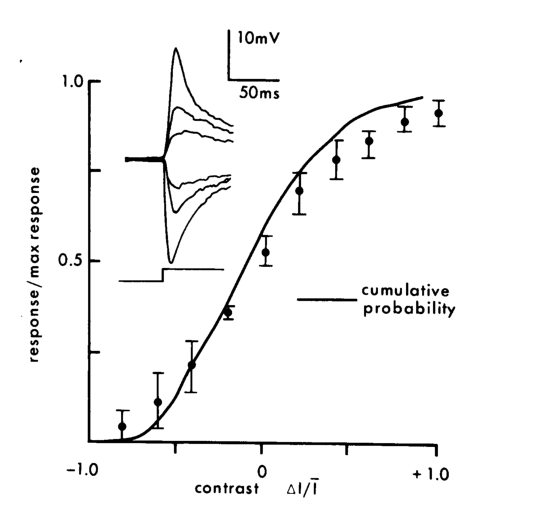
\includegraphics[width=\columnwidth]{figures/laughlin_81.eps}
\label{fig:laughlin}
\caption{The response function of the blowfly LMC closely resembles the cumulative distribution of visual contrasts in its natural environment. Figure taken from Laughlin, S. (1981)}
\end{marginfigure}

This framework can also be generalized to a population of neurons. Writing $O_i$ for the random variable associated with the output activity of each neuron and $O$ for the population activity, we can decompose the redundancy into two terms, yielding
$$
\mathcal{R} = \frac{1}{C} \left(C - \sum_i H(O_i) \right) + \frac{1}{C}\left(\sum_i H(O_i) -H(O)\right).
$$
The first term accounts for redundancy arising from unequal frequency of use of different symbols and the second accounts for redundancy arising from 
correlations between the activities $O_i$. In the example above we have only had to deal with the left term, since we had only one activity and therefore no 
correlations between them. A lot of the efficient coding literature, however, has dealt with the second term, and a number of different approaches have looked 
towards independent components of natural stimuli, assuming that whitening or gain control could account for the maximization of the first term.\par

Michael Lewicki, for example, demonstrated that using independent component analysis\footnote{Indepedent Component Analysis, or ICA for short, tries to 
decompose a signal into a set of features which are statistically independent between them. This can be done by minimization of a number of different cost 
functions.} on a set of natural sounds, comprised of human speech, animal vocalizations and natural background sounds, one recovers receptive fields similar to 
the receptive fields of early auditory neurons.\cite{Lewicki2002} There have been a number of similar studies based on different efficiency measures. 
Another way to interpret Barlow's approach is to eschew information theory and to take the hypothesis that the response of sensory systems seek to represent
in a way that allows for optimal reconstruction while minimising the number of spikes employed. This approach is often called \emph{sparse coding} since the
resulting codes will show response with sparse activity in the neural population. Bruno Olshausen and David Field,\cite{Olshausen1996} for example, have shown 
that, applying the sparse coding approach to a set of natural images results in filters similar to receptive fields in primary visual cortex.\footnote{Sparsity is in 
principle given by the number of active neurons, or if the response is graded by the sum of the activities of the neurons. This leads to cumbersome mathematics
and the kurtosis of the activity is usually employed as a surrogate for the sparsity.}\par

These results and a number of other similar studies have lent considerable traction to the idea that the nervous system is adapted to encode the stimuli present in 
the animal's natural environment. This approach, however, is not without its issues. For one, the limit of Shannon's theorem, in which the redundancy of the code is 
very small, turns the code ever harder to decode. Another important point is that, although minimizing dependence between filters yields good estimates of 
receptive fields observed in the brain, neurons' activities in the brain are far from independent.\footnote{Insert citation about correlations in brain} Though the 
redundancy reduction approach has provided numerous insights as mentioned above, other ideas have emerged since.
\par

\section{The Bayesian Brain}

The finding that humans perform near-optimally\marginnote{Optimality is used in the Bayesian sense, where we mean the subjects integrate uncertain information according to Bayes' rule} when integrating uncertain cues from different senses have led neuroscientists to theorize that the brain explicitly represents distributions over world states.\cite{Ernst2002,Ma2006} In these so-called probabilistic population codes, a spike would contribute to the computation of a posterior probability over world states with a likelihood depending on its conditional probability of firing given the stimulus. This leads to a Bayesian interpretation of the activity of the brain, where the reliability of different sensory cues can be taken in account when integrating them. It can also be argued that representing the uncertainty of events in the world has an important role in decision-making, and will therefore serve as an evolutionary advantage. To use a popular example,\footnote{This example is discussed in \citep{Ma2006}.} let us consider the case of a person deciding wether or not to jump over a stream filled with piranhas. The stream is 1.8 meters wide, and the person jumps an average distance of 2.1 meters. One will be inclined to suggest jumping.\marginnote{Should you jump over a stream filled with piranhas?} Yet both the width of the stream ($w$) as the jumping distance ($j$) are estimated based on uncertain information, and therefore could be imprecise estimates (in the case of the width) or subject to random variation (in the case of the jump distance). Suppose our best guess of the width of the stream is a normal distribution with mean 1.8 meters with a standard deviation of 0.1 meters. Furthermore suppose the standard deviation of the jump distance is 0.4 meters. That would give us a probability of approximately 0.23 of falling down the cliff. So one would definitely be less inclined to jump over the stream, or would at least take preventive actions to minimize the uncertainty in both your estimate of the width of the stream and your jump.\par
From a neural perspective, we could then infer the stimulus distribution (distribution over stream widths) given the response of a neuron population and a model of its response variability. If we assume a given neuron responds according to a certain distribution $P(r|s)$\marginnote{Here we term $r$ the response and $s$ the stimulus}, the Bayesian posterior is given simply by
\[
P(s|r) = \frac{P(r|s) P(s)}{P(r)} \propto P(r|s) P(s).
\]
Assuming independent firing for a number of neurons, whose response distributions are given by $P(r_i|s)$ we would have simply
\[
P(s|\{r_1,\ldots,r_n\}) \propto P(s) \prod_i P(r_i|s).
\]
One then still has to determine the nature of the neural variability given by $P(r|s)$. This distribution is often taken to be Poisson. This means that for very short time intervals, of duration $dt$, the probability of neuron $i$ spiking would be given by a rate function $f_i(s)$, as
\[
P_{dt}(r_i|s) \approx f_i(s) dt.
\]
The true Poisson distribution for spike counts assuming the stimulus does not change during a time interval of duration $T$ is given by\marginnote{Poisson distribution}
\[
P_T(r_i|s) = \frac{e^{-f_i(s) T}f_i(s)^{r_i}}{r_i!}
\]
The rate function $f_i(s)$ is often called the tuning function of the neuron. Given a number of neurons in primary visual cortex responding to the edges of the stream, one could then estimate the stream from those responses according to a simple model as
\[
P(width|{r_1,\ldots}) \propto P(width) \prod_i P(r_i|width),
\]
and likewise obtain the mean and standard deviation of our estimate. More simply we can look for the maximum a posteriori estimator, the value of $s$ that maximises
the probability $P(width|{r_1,\ldots})$. It is often more convenient to maximise the log-probability $\log P(width|{r_1,\ldots})$. Often an additional assumption of a flat
prior is made, yielding the Maximum likelihood estimator.
\par
Note that given a distribution over visual stimuli or a distribution over stream widths, one could seek a set of tuning functions $f_i(s)$ such that the standard deviation 
of our estimate is minimal. This is clearly a very broad formulation of the problem, but it will be the central question studied in this thesis. Alternatively, one could look
directly at the (expected) cost associated with a decision (to jump or not to jump) and choose the set of functions $f_i(s)$ which minimises the future expected cost.
We will investigate the difference between these approaches as well.
\par

Why would an organism be interested in estimating the distribution of world states conditioned on the activity of its sensory systems, though? For one, there is
the finding that the best estimator for the world's state is the mean of the posterior distribution (see \fref{chap:mse}). This means that regardless of the particulars
of the response properties of the sensory system, the posterior mean gives us the world's estimate with the lowest expected quadratic error. A second important
reason is multisensorial cue integration. Let us assume we have a visual and an auditory cue for the width of said stream.\footnote{A foggy view of the opposite 
margin ($v$) and a faint voice talking from the opposite margin ($a$).} Both lead us to different estimates of the stream's width ($\hat{w}_v$ for the visual estimate 
and $\hat{w}_a$ for the auditory estimate). There are countless ways of combining these two to obtain a final estimate of the width. But without further information
on the posterior distributions $P(w|a)$ and $P(w|v)$ we have no way of knowing the best way to combine them. If we had knowledge of them, we could simply
evaluate the full posterior mean\footnote{Assuming the auditory and visual stimuli are uncorrelated conditioned on the world's state.}
\[
\hat{w}_{a,v} = \int dw w P(w|a,v) = \int dw w \frac{P(a|w)P(v|w)P(w)}{P(a)P(v)}.
\]
In the case of Gaussian distributions, we would have $P(w|a) = \mathcal{N}(\hat{w}_a,\sigma_a)$, and $P(w|v) = \mathcal{N}(\hat{w}_v,\sigma_v)$, leading to the simple
cue integration rule
\[
\hat{w}_{a,v} = \frac{\sigma_v \hat{w}_a + \sigma_a \hat{w}_v}{\sigma_a + \sigma_v},
\]
There is no simple formula like this in general, though, leading to the need to estimate the full distribution.
\par


%
%\section{Dynamic Population Coding}
%
%We have had to assume that the stimulus did not change during the response of the neurons to evaluate the Poisson probability of a number of spikes being fired by a neuron. If we relax this assumption, and assume now that the stimulus evolves during time, being now a dynamic stimulus $s(t)$, we will have to reformulate the neural variability model. The probability for infinitesimal time intervals remains the same though. If we denote the number of spikes fired by neuron $i$ since the beginning of the experiment by $N_i(t)$, we can write then
%\[
%P(N_i(t+dt) - N_i(t) = 1|s(t)) = f_i\left(s(t)\right) dt,
%\]
%and 
%\[
%P(N_i(t+dt) - N_i(t) = 0|s(t)) = (1-f_i\left(s(t)\right)) dt.
%\]
%Denoting the limit with $dt\to 0$ of the difference as $dN_i(t)$, we can write the probability of a spike train given by $N_i = \{N_i(\tau), \tau \in [0,T]\}$ conditioned on the stimulus history $s = \{s(\tau), \tau \in [0,T]\}$ as
%\[
%P(N_i|s) = \exp\left(-\int_0^T f_i(s(\tau)) d\tau + \int_0^T \log\left[f_i(s(\tau))\right] dN_i(\tau) \right)/N_i(T)!.
%\]
%We are using the notation of stochastic calculus, where the stochastic integral over a jump process is given by
%\[
%\int f(t) dN(t) = \sum_{t_i} f(t_i) (N(t_i) - N(t_i^-)),
%\]
%where $N(t_i^-) = \lim_{t\uparrow t_i} N(t)$. This can be made rigorous in the language of Martingales but we will keep the discussion simple, as most of the processes
%considered are well behaved Poisson or Wiener processes.
%In that sense we can estimate the probability of the entire stimulus history given a spiking history of a population of neurons as
%\[
%P(s|\{N_1,\ldots,N_n\}) = P(s) \prod_i P(N_i|s),
%\]
%furthermore we can marginalize out all but the present value of $s$ to obtain the filtering probability
%\begin{equation}
%\label{eq:filtering_eq_path}
%P(s(T)|\{N_1,\ldots,N_n\}) = \int d\mu(s\setminus T) P(s) \prod_i P(N_i|s),
%\end{equation}
%where $d\mu(s\setminus T)$ denotes the measure over all paths of the stimulus $s$ ending at the given value of $s(T)$. In all but a few exceptions, we will focus in
%this thesis on the Gaussian measure over paths defined by a Gaussian process. A Gaussian process is a random variable $g$ such that for any set of points in its
%domain $\{t_1, t_2, \ldots , t_N\}$, the distribution of $\{g(t_1), g(t_2), \ldots, g(t_N)\}$ is Gaussian with mean $\{\mu(t_1),\mu(t_2),\ldots,\mu(t_N)\}$ and covariance
%matrix $\left<\left(g(t_i) - \mu(t_i)\right)\left(g(t_j)-\mu(t_j)\right)\right> = K(t_i,t_j)$. $K(u,v)$ is commonly called the Kernel of the Gaussian process. Gaussian 
%Processes, or GP's have been extensively used for numerical regression, smoothing, classification and other uses in machine learning and signal 
%processing \cite{Rasmussen2005}. Simple examples of Gaussian processes are the Wiener process, the Ornstein-Uhlenbeck process and the Radial-Basis-Function
%processes. Gaussian Processes allow for a number of simplifications in practice, and in the case we consider, the posterior distribution can be computed exactly.\par
%In practice, we now need to compute averages of the Poisson likelihood over paths of a Gaussian process. This is general very complicated, and approximations are
%usually employed to decode the stimulus from the spike train.\cite{Ahmadian2011,Ergun2007} Looking at \fref{eq:filtering_eq_path} for the Poisson case we can write
%\begin{align*}
%P(s(T)|\{N_1,\ldots,N_n\}) \propto& \int d\mu(s\setminus T) P(s)\\
%& \exp\left(-\sum_i \int_0^T f_i(s(\tau)) d\tau + \sum_i \sum{t_i} \log\left[f_i(s(t_i))\right]  \right).
%\end{align*}
%There are two terms in the exponent, one referent to the actual occurrence of spikes at the spike times, and one accounting for the absence of spikes in all other 
%instants. If we only had to deal with the actual spike times, the task of inferring the posterior is substantially simpler, as we could perform approximate inference
%over a finite set of points, instead of evaluating averages over all possible paths. This would be the case if the sum of the rates over all neurons was constant, or
%at least independent of the value of the stimulus $s(t)$. This is the dense coding regime, as a dense packing of the tuning curves over the space of the stimulus
%$s$ will lead to a population firing rate which is insensitive to $s$. In that case we would have $\sum_i f_i(s(t)) = C$, and the posterior can be further simplified to
%\[
%P(s(T)|\{N_1,\ldots,N_n\}) \propto \int d\mu(s\setminus T) P(s) \prod_i \prod_{t_i} f_i(t_i).
%\]
%This is often also used as an approximate inference procedure, as accounting for the absence of spikes throughout the duration of the experiments often makes the
%inference problem much harder. We will further simplify the problem by assuming that the tuning functions $f_i$ are unnormalised Gaussians, turning the problem of
%evaluating the posterior into a Gaussian Process Regression problem. This will allow us to treat the evolution of the MSE of the optimal Bayesian estimate for a
%given population of neurons using the language of statistical physics. This had been done similarly for the case of Gaussian Process regression in the smoothing
%case,\cite{malzahn2005statistical} but to the author's best knowledge it had not been studied for the filtering case before. This has allowed us to obtain a number of
%analytic results. The general case, however, must be dealt with numerically, and we review a few techniques for the filtering of stochastic processes under
%general conditions.\par



%The main goal of neuroscience is to answer a simple yet puzzling question: {\em What is the brain doing?} One might argue that we know a lot about what the brain is doing, at least on the phenomenological side, yet the more conceptual levels of what problem the brain is solving, or what it is good at doing, are far from answered. The main analogy we see in use in the field of neuroscience is that of the brain as a computer, hence the frequent use of concepts from Shannon's mathematical theory of communication. Namely, it is frequently hypothesized that the brain is optimally representing interesting aspects of the world it perceives. This thesis seeks to discuss the concept of optimal coding in neural systems. In it, I will discuss mainly findings in filtering of stochastic processes from point process observations and its relation to optimal population coding.\par
%Filtering is of general interest because of its relation to optimal control. More precisely, when considering a linear quadratic control problem under Gaussian noise conditions, the {\em separation principle} holds, and we can design an optimal controller by first predicting the state of the system, and then choosing the optimal control for the noiseless case on that state. The prediction step is solved by the Kalman filter. This framework is frequently used in the study of motor control, and a number of recent experiments and developments have relied on optimal control theory to model the properties of animal subjects under specific noise conditions. Here I will argue that the same approach should also be considered in the sensory areas of the brain.\par
%Investigators have repeatedly hypothesized that the shape of receptive fields and the response properties of sensory neurons can be traced back to optimality with respect to some criterion. The first approach, which drew heavily from Shannon's information theory, was Barlow's efficient coding hypothesis. In its initial form, it stated that the code employed in sensory systems should be adapted to the stimulus distribution in a way to minimized the redundancy, as defined in information theory as the difference between the code capacity and the source entropy divided by the code capacity. Many different efficiency measures have since been proposed. Metabolical considerations favor the use of sparse codes, where at any given time only a few neurons are active.\par
%Another popular approach is to use the Cramer-Rao bound of statistics, and maximize the fisher information of the code, so minimizing a lower bound on the mean-squared-error of the estimator. This has been very popular and is still widely employed in the theoretical neuroscience literature. This bound, however, has been proven to not be tight in useful regimes, and more recently a shift towards using the minimum of the mean-squared-error directly as an efficiency measure has been taking place. We focus here on this measure of efficiency, which we will motivate through optimal control theory in chapter ?? (INSERT REFERENCE).\par
%An alternative approach, which is still in its budding phase, is to consider directly optimal control problems and from the average cost incurred by a given code, choose an optimal code for a given task. This is hindered by the considerable analytical problems involved in treating optimal control problems analytically. I will show, however, that in the popular framework of dense Gaussian tuning functions, an exact expression can be found for the optimal cost-to-go of a linear-quadratic-Gaussian control problem. This bypasses the somewhat abstract notion of an efficiency criterion to consider directly the costs of a given code to the animal using it. It does so at the considerable expense of oversimplifying the problems faced by an animal to an impressive amount. Yet, the approach considers the problem of optimal coding from a more holistic perspective, considering representation and coding as a cog in a machine rather than and end in itself.\par
%
%\section{Structure}
%
%I will start out by reviewing the literature and the different approaches to optimal population coding in chapter ??, giving special attention to the case of mean-squared-error minimization which is considered in this thesis. In the following chapter, I briefly introduce the theory of filtering of point-process observed stochastic processes. Here, the general theory of filtering is presented and the simplifications introduced by the dense Gaussian tuning function limit are discussed. In the following chapter, I discuss results on the mean-squared-error in filtering of Gaussian processes, providing analytical results and comparing it to simulations. The derivations are also compared with a replica-type approach which yields the same results. In the following chapter I consider the problem of optimal control using point-process observations. This is discussed briefly, and a derivation for the optimal cost-to-go is presented. Finally, I consider the implications of the approaches developed to a ecological theory of sensory processing. Namely, I consider the relationship between optimal tuning widths and firing rates with the timescales and correlation lengths in the processes. This is also done numerically for a number of cases that are analytically intractable. I finalize by discussing the presented research, its impact and relation to previous research and future directions of research.
%\cite{susemihl2011}

%We will argue that filtering of stochastic processes is a good proxy for the neural representation of stimuli in the brain.\par

%This presents a number of problems, which we will address in this thesis.

\chapter{Filtering and Prediction with Point Process Observations}

\label{chap:filtering}

\epigraph{Prediction is very difficult, especially about the future.}{Niels Bohr}

In the Introduction I described the general framework in which I seek to study optimal population coding. To do so in a dynamic setting, one must first develop the theory
of temporal estimation of dynamic stimuli from point processes. This is a surrogate for the functioning of a neural population receiving information from the encoder.
There are a number of cases in which the filtering problem can be solved exactly, and I will discuss results from the theory of optimal filtering. In the cases where the
optimal filter is intractable or too expensive to evaluate exactly, I will present methods to approximate the posterior density.\par

In the neuroscientific context, the process $X(t)$ being estimated or filtered would correspond to some environmental feature of interest to a sensory system of some organism, while
the signal would be some neural response coming from a neural population. As was mentioned in \fref{sec:framework}, one example would be to estimate the presence of a moving
grating from the response of retinal ganglion cells. In that sense, the ganglion cells provide a noisy representation of an environmental variable of interest to some downstream
cortical area (V1 for example). In this chapter I will discuss methods to infer the value of the sensory stimulus from the noisy response of a population of neurons.

\section{A Note on Stochastic Processes}

\label{sec:stochastic_proc}

Throughout this thesis, I will repeatedly talk about stochastic processes and the framework of stochastic calculus, so I will provide a short introduction to stochastic processes and
the theory of stochastic calculus. In the study of ordinary differential equations, one works with equations such as
\[
\frac{d x}{dt} = f(x),
\]
which are solved by
\[
x(t) = x(0) + \int_0^t f(x(u),u) du.
\]
This can be modified to include a white-noise term in the evolution of $x(t)$, leading to the Langevin equation
\[
\frac{d X}{dt} = f(X,t) + \sigma(X,t) \xi(t),
\]
where $\sigma(X(u),u)$ is a state- and time-dependent strength and $\xi(t)$ is a {\em rapidly fluctuating random term}, i.e.\mycite{Gardiner2004}
$$\boldsymbol{E}[\xi(t)] = 0\textrm{ and }\boldsymbol{E}[\xi(t)\xi(s)] = \delta(t-s).
$$ 
This approach is 
problematic, however, since the process $X(t)$ thus defined is not differentiable, rendering the Langevin equation mathematically inconsistent. One can, however, extend the solution 
to the deterministic case as
\footnote{Note that because of the new definition, $X(t)$ is now a random variable, hence
the upper-case notation.}
\[
X(t) = X(0) + \int_0^t f(X(u),u) du + \int_0^t \sigma(X(u),u) \xi(u) du.
\]
$\xi(u)du$ can be shown to be equal to $dW(u) = W(u+dt)-W(u)$ in the limit $dt \to 0$, which leads to the usual It\=o stochastic integral
\[
X(t) = X(0) + \int_0^t f\left(X(u),u\right) du + \int_0^t \sigma\left(X(u),u\right) dW(u).
\]
The stochastic integral can be shown to exist as long as the functions $f$ and $\sigma$ are continuous and non-anticipating.\footnote{A function $G(t)$ is said to be non-anticipating 
with  respect to a stochastic process $X$ if it is statistically independent of values of $X(s)$ for $s>t$. Simply put, $G_n(t) = \int_0^t dW(s)$ is non-anticipating with respect to $W(s)$, but
$G_a(t) = \int_0^{2t} dW(s)$ is not.} One usually writes the evolution of $X(s)$ in terms of a stochastic differential equation, instead of a stochastic integral. The process $X(t)$ 
described above would obey the SDE
\[
dX(t) = f\left(X(t),t\right) dt + \sigma\left(X(t),t\right) dW(t).
\]
This is just a shorthand for the stochastic integral, and has no precise mathematical interpretation, as the terms are of different orders. More specifically, the term $dW(t)$ is of the 
order of $\sqrt{dt}$ while the first term is of order $dt$. In an analogy to the study of classical mechanics, the first term is often called the drift of $X(t)$ and the second the diffusion.
\par

Processes $X(s)$ defined in this way are continuous. Often, however, one wants to model a stochastic process which incurs discontinuous jumps as well. I can for that purpose 
introduce a third term in the definition of $X(t)$. Let $j(X(t),t)$ be a function that describes the size of the jump the process experiences at time $t$ and state $X(t)$. 
If these jumps occur at some set of random times $\{t_i\}$, the process $X(t)$ can be written as
\[
X(t) = X(0) + \int_0^t f\left(X(u),u\right) du + \int_0^t \sigma\left(X(u),u\right) dW(u) + \sum_{t_i <t} j\left(X(t_i^-),t_i\right),
\]
where I have defined
$$
X(t^-) \equiv \lim_{s \uparrow t} X(s),
$$
as the limit of $X(t)$ from the left. The jumps in $X(t)$ should be modulated by the point where they originate, not their
destination, so this definition makes intuitive sense.
Let $N(t)$ be then given by
\[
N(t) = \sum_{t_i} \Theta(t-t_i) = \int_0^t \sum_i \delta(u-t_i) du\equiv \int_0^t dN(u), 
\]
where $\Theta(x)$ is the Heaviside step function. With this definition, I can then write
\[
X(t) = X(0) + \int_0^t f\left(X(u),u\right) du + \int_0^t \sigma\left(X(u),u\right) dW(u) + \int_0^t j\left(X(u),u\right) dN(u).
\]
Throughout the text I will also employ an SDE notation for this integral as follows
\begin{equation}
\label{eq:full_stoc}
dX(t) = f\left(X(t),t\right) dt + \sigma\left(X(t),t\right) dW(t) + j\left(X(t^-),t\right) dN(t).
\end{equation}
\par
This encompasses all the stochastic processes I will consider in this text. What happens to a function of a stochastic variable that changes over time, though? Say I want to evaluate
some function of $X(t)$, say $g(X(t),t)$, how does this function vary in time? It\=o's lemma tells one how to find the variation in $g$ from the process $X(t)$. If $X(t)$ evolves according
 to \fref{eq:full_stoc}, we have\footnote{For a more full derivation, see \mycitep{Sennewald2006} or \mycitep{privault2014}.}
\begin{align*}
 dg \equiv& \lim_{dt \to 0} \left[g(X(t+dt),t+dt) - g(X(t),t)\right]\\
 =& \left(\partial_t g + \partial_x g^\top\, f(X(t),t) +\frac{1}{2}\Tr\left[ \sigma\sigma^\top \partial^2_x g\right]\right) dt+ \partial_x f^\top \sigma(X(t),t) dW(t) \\
 &+ \left(g(X(t^-)+j(X(t^-,t),t)-g(X(t^-),t)\right)dN(t),
 \end{align*}
 where I am using the notation
 $$\partial_x g = \left(\frac{\partial g}{\partial x_1},\ldots, \frac{\partial g}{\partial x_N}\right)^\top$$
 and 
 $$
 (\partial^2_x g)_{i,j} = \frac{\partial^2 g}{\partial x_i \partial x_j}.
 $$
This is, again to be understood as a stochastic integral, where we have
\begin{align*}
g(X(t),t) =& g(X(0),0) + \int_0^t \left(\partial_t g + \partial_x g^\top f(X(u),u) +\frac{1}{2}\Tr\left[ \sigma\sigma^\top \partial^2_x g\right]\right) du \\
&+ \int_0^t \partial_x f^\top \sigma(X(u),u) dW(u) +\int_0^t \left(g(X(u^-)+j(X(u^-,u),u)-g(X(u^-),u)\right)dN(u).
\end{align*}
This is in stark contrast of the usual change of variables formula for differentiable variables $y(t)$, where we would have
\[
dg\equiv \lim_{dt \to 0} \left[g(y(t+dt),t+dt) - g(y(t),t)\right]= \left(\partial_t g + \partial_y g^\top \, \partial_t y \right)dt.
\]

\subsection{The Evolution of Probabilities}

Another important question, is how $X(t)$ is distributed at some time $t$ if it is initially at some point $x_0$ at time $0$.\footnote{Or distributed according to some distribution $P_0(X)$ at time $0$.} It is useful for that problem to consider the transition probability
density
$$
P(X(t+dt)\in A | X(t)) = \int_A p(x,t+dt|X(t),t).
$$
Let me define three sources of change arising from the transition density $p$. For any $\varepsilon > 0$ I will assume the limits below exist
\begin{subequations}
\begin{equation}
\lim_{dt\to 0} p(x,t+dt|z,t)/dt = W(x|z,t), \forall x,z,t, \textrm{ s.t } |x-z| \ge \varepsilon,
\end{equation}
\begin{equation}
\lim_{dt\to0} \frac{1}{dt} \int_{|x-z| \le \varepsilon} dx (x-z) p(x,t+dt|z,t) = A(z,t) + O(\varepsilon),
\end{equation}
\begin{equation}
\lim_{dt\to0} \frac{1}{dt} \int_{|x-z| \le \varepsilon} dx (x-z)(x-z)^\top p(x,t+dt|z,t) = B(z,t) + O(\varepsilon).
\end{equation}
\end{subequations}
These terms define the contribution of jumps ($W(x|z,t)$), drift ($A(z,t)${ and diffusion ($B(z,t)$) to the transition density of the process $X(t)$. It is straightforward to show that, if $X(t+dt)$ is given by $X(t) + dX(t)$ as in \fref{eq:full_stoc}, then $A(z,t) = f(z,t)$ and
$B(z,t) = \sigma(z,t)\sigma(z,t)^\top$. I have not defined the distribution of $dN(t)$, but assuming $N(t)$ is a Poisson process with rate $\lambda$, the jump term will be simply $$W(x|z,t) = \lambda \delta(x-z+j(z,t)).$$ With these definitions in hand, it can be shown that the probability density $p$ will evolve according to the differential Chapman-Kolmogorov equation
\begin{align}
\frac{\partial p(x,t|x_0,0)}{\partial t}=& -\nabla \cdot \left(A(x,t) p(x,t|x_0,0)\right) + \frac{1}{2}\sum_{i,j} \frac{\partial^2}{\partial x_i \partial x_j} \left[B_{ij}(x,t) p(x,t|x_0,0)\right]\nonumber\\
+&\int dz \left[W(x|z,t) p(z,t|x_0,0) - W(z|x,t) p(x,t|x_0,0)\right]
\end{align}
The first line corresponds to the terms found in the Fokker-Planck equation, while the second line corresponds to the terms found in the Master equation. These equations are usually
used to describe drift-diffusion and pure jump processes respectively. The differential Chapman-Kolmogorov equation generalises both equations to processes with drift, diffusion
and jumps.\footnote{For a full account of the differential Chapman-Kolmogorov equation, see \mycitep{Gardiner2004}.}

\subsection{Smooth Markovian Processes}

The stimuli defined by SDE's like \fref{eq:full_stoc} will often yield sample paths which are not differentiable. I am, however, interested in using the theory of stochastic processes
to describe the natural stimuli a sensory system encounters in its environment, so it makes sense to consider smooth, differentiable processes as well. \mycitet{Huys2007} looked at
a number of Gaussian processes which yield smooth sample paths. I will here consider a type of process which I shall call the Matern process throughout this thesis.\footnote{I will call 
these processes Matern processes because their autocorrelation $k(t,u) = \boldsymbol{E}[X(t)X(u)]$ are given by the Matern kernel described in \mycitep{Rasmussen2005}.} Symbolically, 
one can write these processes as
\[
\left(\frac{d}{dt} + \gamma\right)^P X(t) = \eta \frac{dW(t)}{dt},
\]
where $P$ is the order of the process. Clearly, this notation is not precise, since the Wiener process $W(t)$ is not differentiable. This can be written as a system of SDE's as
\[
\dot{X}_1(t) = X_2(t),\qquad \ldots, \qquad\dot{X}_{P-1}(t) = X_{P}(t),\qquad  dX_{P}(t) =- \sum_{i=1}^{P} \gamma^{P+1-i} X_i dt + \eta dW(t).
\]
If $P=1$, this gives the one-dimensional Ornstein-Uhlenbeck process. If I take $P>1$, however, $X_1(t)$ will be a smooth random process, as can be seen in
\fref{fig:stoch_example}. $X_1(t)$ itself is no longer a Markov process, as its evolution depends on its time derivatives as well as of its state. It is, however, possible to embed the
process $X_1(t)$ in a $P$-dimensional space, along with its $P-1$ first derivatives, rendering it Markov again. In \mycitep{Susemihl2013} I have used this to study the MMSE of smooth
processes. In this way, all the tools of stochastic dynamics are still available, but one can consider smooth processes, more similar to the ones observed in nature.\par

When studying a population of neurons responding to such an embedded smooth process ${X}(t) = \left(X_1(t),\ldots, X_{P}(t)\right)^\top$, I will mostly consider tuning
functions which only depend on the original smooth process given by $X_1(t)$, which leads to the same filtering process considered in \mycitep{Huys2007}.

\subsection{Infinitesimal Generator of a Stochastic Process}

The infinitesimal generator of a stochastic process is defined as the operator
\[
\mathcal{A} f(x) = \lim_{dt\to 0} \frac{\boldsymbol{E}\left[f(X(t+dt))|X(t)=x\right] -f(x)}{dt}.
\]
The adjoint of this operator is defined as the operator $\mathcal{A}^\dagger$ satisfying
\[
\int (\mathcal{A} f(x)) g(x) dx = \int f(x) (\mathcal{A}^\dagger g(x)) dx.
\]

\section{Estimation and Filtering}

Estimation is the field of statistics that deals with the inference of some unknown variable from uncertain observations of that variable. It can be best described by an example. Given a pair of variables $X$ and $Y$, and a model for their relationship, say $P_Y(y|X=x)$, one could infer the value of $X$ from observations of $Y$. Using Bayes' rule one obtains
\[
P_X(x|Y=y) = \frac{P_X(x)P_Y(y|X=x)}{P_Y(y)},
\]
which can be used to estimate the value of $X$.
I will be mostly concerned with temporal processes, say a random process $X(t)$ which needs to be inferred from observations of a 
dependent process $Y(t)$. When one is interested in inferring $X(t)$ from data $\{Y(s)\},\,s \in [0,T]$, the problem gets named according 
to the value of $t$. If $t \in [0,T]$, it is called a \emph{smoothing} problem. If $t = T$, it is called a \emph{filtering} problem. If $t>T$, it is called a \emph{prediction} or 
\emph{forecasting} problem.\marginnote{Smoothing, filtering and predicting.} The temporal structure of the processes leads to correlations in the variables being 
estimated ($X(s)$ for different values of $s$), and there a number of ways to take advantage of this. I will look into the theory of filtering of 
diffusion processes observed through a second diffusion process dependent on the first and then turn to the theory of filtering of diffusion processes observed through 
doubly stochastic point processes.

\subsection{Kalman Filtering}
\label{sec:kalman}
Let me consider a more concrete setting. Suppose one is dealing with a system that evolves according to a stochastic discrete-time dynamics given by
\[
X(t+1) = A X(t) + H^{1/2} N_t.\footnotemark
\]
\footnotetext{$H^{1/2}$ indicates the Cholesky decomposition of the positive-definite (or semi-definite) matrix $H$. The exponent $1/2$ is used because $H^{1/2} \left(H^{1/2}\right)^\top = H$.}
We take $X(t) \in \mathbf{R}^n$, $A\in \mathbf{R}^{n*n}$ and $H \in \mathbf{R}^{n*n}$ positive-definite. $N_t$ is a normal n-dimensional random variable with zero mean and unit standard deviation. Suppose now we observe a process $Y(t)$ given by
\[
Y(t) = C X(t) + D^{1/2} M_t,
\]
where $C \in \mathbf{R}^{m*n}$, $Y(t) \in \mathbf{R}^m$ and $D\in \mathbf{R}^{m*m}$ positive-definite. $M_t$ is as before a normal $m$-dimensional random variable 
with zero mean and unit standard deviation. The filtering problem is to determine an estimate of $X(t)$ given observations of $Y(1),Y(2),\ldots,Y(t)$. This can done by a 
recursive estimation procedure first proposed by Rudolf E. K\'alm\'an. Namely, for each time step, one first predicts the conditional distribution of $X(t)$ given our estimate 
of $X(t-1)$ and then corrects that according to the observation $Y(t)$. One can easily obtain recurrence relations for this filtering problem by noting how the mean and 
variance of $X(t)$ evolve. One has
\[
\boldsymbol{E}\left[X(t+1)\middle| \mu(t),\Sigma(t)\right] = A\boldsymbol{E}\left[X(t)\right],
\]
and
\[
\boldsymbol{E}\left[X(t+1)X(t+1)^\top\middle| \mu(t),\Sigma(t)\right] = A\boldsymbol{E}\left[X(t)X(t)^\top\right]A^\top + H,
\]
which leads clearly to
\[
\boldsymbol{E}\left[X(t+1)X(t+1)^\top\middle|\mu(t),\Sigma(t)\right] - \boldsymbol{E}\left[X(t+1)\middle| \mu(t),\Sigma(t)\right] \boldsymbol{E}\left[X(t+1)\middle| \mu(t),\Sigma(t)\right] ^\top = A\Sigma(t)A^\top +H.
\]
So, in the absence observations, if knowledge of $X(t)$ was given by $\mathcal{N}(\mu(t),\Sigma(t))$, the distribution over $X(t+1)$ before the observations 
is\footnotemark  $$\mathcal{N}(A\mu(t),A\Sigma(t)A^\top+H).$$After observing the value of $Y(t+1)$, one can update the distribution through Bayes' rule as
\[
P(X(t+1)| Y(t+1), \mu(t),\Sigma(t)) =\frac{P(Y(t+1)|X(t+1))P(X(t+1)|\mu(t),\Sigma(t))}{P(Y(t+1)|\mu(t),\Sigma(t))}.
\]
Here I have dropped the verbose notation of $P_{X(t+1)}(x|Y(t+1)=y;\mu(t),\Sigma(t))$, and have written that simply as $P(X(t+1)| Y(t+1), \mu(t),\Sigma(t))$. The 
meaning should be clear from the context. Furthermore, the distribution $P(X(t+1)|\mu(t),\Sigma(t))$ is given by the Chapman-Kolmogorov equation as\footnotetext{$\mathcal{N}(\mu,\Sigma)$ denotes the normal probability density function with mean $\mu$ and covariance $\Sigma$. The density function is given by
\[
\mathcal{N}(\mu,\Sigma) = \frac{1}{(2\pi)^{N/2} |\Sigma|^{1/2}} e^{-\frac{1}{2} (x-\mu)^\top \Sigma^{-1} (x-\mu)},
\]
where $N$ is the dimension of $x$, and $|\Sigma|$ is the determinant of the covariance matrix $\Sigma$.}
\[
P_{X(t+1)}(x|\mu(t),\Sigma(t)) = \int dz P_{X(t+1)}(x|X(t)=z) P_{X(t)}(z|\mu(t),\Sigma(t)),
\]
leading to the relations derived above.
Note that both terms in the numerator of the Bayesian update are Gaussian distributions and the denominator does not depend on $X(t+1)$, so one can simply find the 
mean and covariance by looking at the exponents in the numerator. The log probabilities are
\[
\log\left[ P(Y(t+1)|X(t+1))\right] = -\frac{1}{2}( Y(t+1) - C X(t+1))^\top D^{-1}(Y(t+1)-C X(t+1)) + \textrm{normalization terms}
\]
and
\[
\log\left[ P(X(t+1)|\mu(t),\Sigma(t))\right]= -\frac{1}{2}(X(t+1) - A \mu(t))^\top (A\Sigma(t)A^\top + H)^{-1} (X(t+1) - A\mu(t)) +\textrm{normalization terms}.
\]
Collecting terms one obtains
\[
\log\left[ P(X(t+1)|Y(t+1),\mu(t),\Sigma(t))\right] = -\frac{1}{2}( X(t+1) - \mu(t+1))^\top \Sigma(t+1)^{-1} (X(t+1)-\mu(t+1)) + \textrm{normalization terms},
\]
where
\[
\Sigma(t+1) = \left(\left(A\Sigma(t)A^\top+H\right)^{-1} + C^\top D^{-1}C \right)^{-1}
\]
\[
\mu(t+1) = A\mu(t) + \Sigma(t+1) C^\top D^{-1}  (Y(t) -C A\mu(t)).
\]
This formulation leads to somewhat cluttered recurrence relations. In the theory of Kalman filtering these are usually broken down into subsequent prediction and correction steps. The notation usually employed in filtering theory is to write $\mu_{t|t-1}$ and $\Sigma_{t|t-1}$ for the mean and covariance of the distribution $P(X(t)|\mu({t-1}),\Sigma({t-1}))$,\footnote{the prediction step} and $\mu_{t|t}$ and $\Sigma_{t|t}$ for the mean and covariance of the updated distribution $P(X(t)|Y(t))$.\footnote{the correction step} One can write simply
\begin{eqnarray*}
\mu_{t+1|t} = &A\mu_{t|t},\\
\Sigma_{t+1|t} = & A\Sigma_{t|t}A^\top + H.
\end{eqnarray*}
Defining the innovation term $Z(t+1)$, and its covariance by
\begin{eqnarray*}
Z_{t+1} = & Y(t+1) - C \mu_{t+1|t}\\
S_{t+1} = & C\Sigma_{t+1|t}C^\top + D.
\end{eqnarray*}
The \emph{optimal Kalman gain}\marginnote{The term \emph{optimal Kalman gain} is usually employed in filtering theory, as it is the matrix $K$ that gives the minimum variance unbiased estimator of $X(t)$ given $Y(t)$.} will be
\begin{eqnarray*}
K_{t+1} = \Sigma_{t+1|t} C^\top S_{t+1}^{-1}
\end{eqnarray*}
and the posterior mean and covariance can be written as
\begin{eqnarray*}
\mu_{t+1|t+1} =& \mu_{t+1|t} + K_{t+1} Z({t+1})\\
\Sigma_{t+1|t+1} =& \left(I-K_{t+1} C\right) \Sigma_{t+1|t}
\end{eqnarray*}
It is relatively simple to show that these relations are equivalent to the ones derived above.\par
The Kalman filter is a fundamental tool in engineering and signal processing and has been used in anything from radar signal analysis to computer vision tracking and 
space expeditions. The list of applications is enormous, and I will only mention three examples. One application is to use the Kalman filter to estimate the current 
position of an object in a navigation system (see \mycitep{kalmannavigation}). Another interesting application is the monitoring of positional measurements through a radar. 
The nature of radar measurements lends itself nicely to this formalism and the Kalman filter has been used extensively in these kinds of applications (see 
\mycitep{kalmanradar}). These are classical examples, but the applicability of the Kalman filter is very widespread, and one can find examples of applications in unexpected 
fields, such as the estimation of future retail sales (see \mycitep{kalmansales}).\par
It has a number of limitations, though. First, note that it requires the knowledge
of the matrices governing the system's dynamics. If the system is governed by linear dynamic and the matrices are known, the Kalman filter provides the exact posterior 
probability. If these are unknown, however, one is forced to estimate them from data, and in the mismatched case\marginnote{The mismatched case refers to the
situation where the parameters of the system are unknown, and we are forced to use a model with parameters mismatched to the system's parameters.} the Kalman 
filter is an approximate method, and can lead to poor results. A number of extensions to the Kalman filter exist, such as the 
extended Kalman filter, the unscented Kalman filter and others. More recently sequential Monte Carlo Markov Chain methods known as particle filters have been a 
subject of great interest as they overcome a number of limitations of Kalman filters, mainly through sampling from many hypothetical system paths for $X$ and
reweighing them to account for the observations.\mycite{doucet2001}


\subsection{Continuous Time: The Kalman-Bucy Filter}

The Kalman filter deals with discrete time systems and can be easily extended to continuous time systems. Though it can be rigorously proved that the derived filter 
equations are rigorous using stochastic calculus, I will only provide an informal derivation.Consider a linear stochastic differential 
equation, say
\begin{equation}
\label{eq:OU_sde}
dX(t) = A X(t) dt + H^{1/2} dW(t),
\end{equation}
where $W(t)$ is a Wiener process. Note that the correspondence with the discrete time case can be simply made by taking $A'=I - A dt$ and 
$H'^{1/2} = \sqrt{dt} H^{1/2}$. The obvious extension for the observation process to continuous-time would be
\[
Y(t) = CX(t) + N(t),
\]
where $N(t)$ is a Gaussian random variable with unit variance for each time $t$. This would, however, render the observation process discontinuous almost 
everywhere. It makes sense to require the observation process to be continuous as well, and a simple way to achieve is to take a process $Y(t)$ evolving according
to the SDE\marginnote{SDE: Stochastic Differential Equation}
\begin{equation}
dY(t) = C X(t) dt + D^{1/2} dV(t),
\end{equation}
where $V(t)$ is a second Wiener process independent of $W(t)$. Note that, unlike its discrete time counterpart, here $Y(t+dt)$ does not only depend on $X(t)$ but also on $Y(t)$. That does not make the analysis much more complicated though, as one can write the inference in terms of $dY(t)$ just as well.\par
One can proceed as in the case of discrete time with a small time increment $dt$ and then pass to the limit of $dt\to 0$. This will lead to
\[
\mu_{t+dt|t} = (I+A dt)\mu_{t|t},
\]
and
\[
\Sigma_{t+dt|t} = \Sigma_{t|t}  + \left(A\Sigma_{t|t} + \Sigma_{t|t} A^\top + H\right) dt.
\]
The distribution of $Y(t+dt)$ in turn is given by
\[
P(Y(t+dt)|Y(t),X(t)) = \mathcal{N}\left(Y(t) + C\,X(t)\, dt, D\, dt\right),
\]
or more simply one can directly write down the distribution of $dY(t)$,
\[
P(dY(t)|X(t)) = \mathcal{N}\left(C\,X(t)\,dt,D\,dt\right).
\]
The Bayes' update will be
\[
P(X(t+dt)|dY(t+dt)) = \frac{P(dY(t+dt)|X(t+dt)) P(X(t+dt)|X(t))}{P(dY(t+dt))}. %\propto \mathcal{N}\left(C\,X(t+dt)\,dt,D\,dt\right)\mathcal{N}\left(\mu_{t+dt|t},\Sigma_{t+dt|t}\right).
\]
The product of Gaussians will lead to a Gaussian with variance
\[
\Sigma_{t+dt|t+dt} = \left(\Sigma_{t+dt|t}^{-1} + C^\top D^{-1} C dt \right)^{-1},
\]
which can be Taylor expanded to
\[
\Sigma_{t+dt|t+dt} = \Sigma_{t+dt|t} - dt \Sigma_{t+dt|t} C^\top D^{-1} C \Sigma_{t+dt|t} + o(dt^2).
\]
Inserting the expression for $\Sigma_{t+dt|t}$ and taking the limit for $dt \to 0$ one obtains the filter equations for $\mu(t) \equiv \mu_{t|t}$ and $\Sigma(t) \equiv \Sigma_{t|t}$. The posterior variance obeys the ordinary differential equation
\begin{subequations}
\label{eq:kalman_bucy}
\begin{equation}
\frac{d \Sigma}{dt} = A\Sigma(t) + \Sigma(t) A^\top + H - \Sigma(t) C^\top D^{-1} C\Sigma(t).
\end{equation}
The posterior mean, however, is still a stochastic variable, as it is dependent on the diffusion process $Y(t)$. $\mu(t)$ obeys the SDE
\begin{equation}
d\mu(t) = A\mu(t) + \Sigma(t) C^\top D^{-1} \left( dY(t) - C\mu(t) dt \right).
\end{equation}
\end{subequations}
The structure of the equations is very similar to the Kalman updates for discrete-time, as the dynamics of the mean only incorporates the observations through 
an innovation process.\par

\subsection{Kushner-Stratonovich Equation}

In the cases above I could restrict myself to study the mean and covariance because of the linear structure of both the system dynamics and the observation 
dynamics. In the general case, however, one can not restrict herself to these moments. In the worst-case scenario one can not escape from estimating the full posterior 
distribution $P(x,t) = P_{X(t)}(x|Y_{0:t},X(0) = x_0)$\marginnote{$Y_{0:t}\equiv \{Y(s), 0\le s \le t\}$}  at every time step.\par
For a Markov system with infinitesimal generator $\mathcal{A}$, the unobserved probability 
density obeys
\begin{equation}
\label{eq:kolmogorov_fw}
\frac{\partial P(x,t)}{\partial t} = \mathcal{A}^\dagger P(x,t),
\end{equation}
where $\mathcal{A}^\dagger$ is the adjoint of $\mathcal{A}$. If the observation process $Y(t)$ evolves according to
\[
dY(t) = c(X(t)) dt + D^{1/2} dV(t),
\]
then, defining $\hat{c}_t = \int dx\, c(x) P(x,t)$, the posterior distribution obeys the stochastic partial differential equation\footnote{Here I am using a definition analogous
to the definition of $dX(t)$ for a partial difference with respect to time. We have
\[
d_t P(x,t) = \lim_{dt\to 0} \left[P(x,t+dt)-P(x,t)\right].
\]}
\begin{equation}
\label{eq:kushner}
d_t P(x,t) = \mathcal{A}^\dagger P(x,t) dt + (c(x) - \hat{c}_t)^\top D^{-1} (dY(t) - \hat{c}_t dt) P(x,t).
\end{equation}
\Fref{eq:kushner} is usually called the Kushner equation or the Kushner-Stratonovich equation in honor of Harold J. Kushner and Ruslan Stratonovich, the statisticians 
who first derived it. It is not hard to demonstrate that, by taking $c(X(t)) = C X(t)$ we can recover \fref{eq:kalman_bucy} above for the evolution of the moments 
according to \fref{eq:kushner}.\mycite{Bucy1965} These equations, as one can 
imagine, are very hard to solve exactly, and approximate solutions are usually employed. The techniques collectively called particle filters seek to generate
sample paths $Z(t)$ where the distribution of $Z(t)$ is given by the solution of the Kushner equation. Through a sequential sampling and reweighing procedure
this can be done without solving \fref{eq:kushner} explicitly.
 
\section{Filtering of Poisson Process Observations}
 
The theory of filtering of diffusion processes can be extended to the case of Poisson processes as well. Donald Snyder has derived an equation for the filtering of stochastic processes observed through doubly stochastic Poisson processes which bears a remarkable resemblance to \fref{eq:kushner}.\mycite{Snyder1972} A Poisson process can be defined as a counting process $N(t)$ such that the transition probabilities for infinitesimal times $dt$ are given by
\begin{subequations}
\begin{equation}
P(N({t+dt})-N(t) = 0 ) = 1 -\lambda dt + o(dt^2)
\end{equation}
\begin{equation}
P(N(t+dt)-N(t) = 1) = \lambda dt + o(dt^2)
\end{equation}
\begin{equation}
P(N(t+dt)-N(t)>1) = o(dt^2)
\end{equation}
\begin{equation}
P(N(t+dt)-N(t)<0) =0
\end{equation}
\end{subequations}
In the limit of $dt\to 0$, the transition probabilities for $N_t$ are completely determined by $\lambda$, the rate of the process. \Fref{fig:poisson_example} shows examples of samples from a Poisson process $N_t$ with different rates.
\begin{marginfigure}
\includegraphics[width=\columnwidth]{figures/figure_2_1.pdf}
\caption[Samples of Poisson Processes.]{Samples of Poisson processes with rates equal to $0.5, 1.0$ and $2.0$.}
\label{fig:poisson_example}
\end{marginfigure}
\par
A doubly stochastic Poisson process, is a process where the rate $\lambda$ is itself a stochastic random variable, usually a function of another stochastic process
$X(t)$. In the case first considered by Snyder, the observations were particle counts of radioactive decay for medical diagnostics. The rate was a function of the 
concentration of the radioactive substance administered to the patient, and by observing particle counts through time onewould like to infer the concentration of 
radioactive substance in the patient's organs. The temporal aspect was relevant because of the fast decay of the radioactive particles. In that case one will have
\begin{subequations}
\begin{equation}
P(N({t+dt})-N(t) = 0 |X(t)) = 1 -\lambda(X(t)) dt + o(dt^2)
\end{equation}
\begin{equation}
P(N({t+dt})-N(t) = 1|X(t)) = \lambda(X(t)) dt + o(dt^2).
\end{equation}
\end{subequations}
The conditional probability of a path $N_{0:t}$ given a path $X_{0:t}$ is then
\begin{equation}
\label{eq:dspp_likelihood}
P(N_{0:t}| X_{0:t}) = \exp\left[ -\int_0^t \lambda(X(s)) ds + \int_0^t \log(\lambda(X(s))) dN(s) \right],
\end{equation}
where I have used the definition of the stochastic integral with respect to a jump process given in \fref{sec:stochastic_proc}.
Defining the jump points $t_i$ as the points where $\lim_{t\downarrow t_i}N(t) \neq \lim_{t\uparrow t_i} N(t)$, one can write the usual formula for the Poisson density of spike times
\[
P(\{t_i\}|X_{0:t}) =   \exp\left[ -\int_0^t \lambda(X(s)) ds \right]\prod_i \lambda(X({t_i})).
\]
Armed with a rate model for the DSPP\marginnote{DSPP: Doubly Stochastic Poisson Process}, one can infer the stimulus history from the count history. The posterior distribution for $X_{0:t}$ is
\begin{equation}
\label{eq:dspp_post}
P(X_{0:t}|N_{0:t}) \propto P(X_{0:t})  \exp\left[ -\int_0^t \lambda(X(s)) ds + \int_0^t \log(\lambda(X(s))) dN(s) \right].
\end{equation}
$P(X_{0:t})$ is a prior distribution over paths of $X(t)$, which in turn are infinite-dimensional objects. This determines the temporal structure of the stimulus, and can be 
tuned to reflect the statistical properties of the stimuli being considered. In practice, it is very hard to compute the full posterior, and for inference purposes, one generally
deals with a  discretised version of the path.\par

Discretising $X_{0:t}$ one can treat the problem of inferring the paths as a multidimensional estimation problem. The simplest way to estimate $X_{0:t}$ is maximum 
likelihood\marginnote{ML = maximum likelihood} whereby one maximises the likelihood given in \fref{eq:dspp_likelihood}. The function given by \fref{eq:dspp_likelihood}
is called a likelihood for $X_{0:t}$ since it does not define a probability density for it. Further, one can incorporate prior beliefs about 
the structure of $X(s)$ by using the full posterior given in \fref{eq:dspp_post}. Taking the value of $X_{0:t}$ that maximises the posterior probability yields the so-called 
\emph{Maximum a Posteriori} estimator.\marginnote{MAP = maximum a posteriori} The full Bayesian approach would be to take the posterior mean as an estimate for 
$X_{0:t}$, that is one takes the mean of the distribution given in \fref{eq:dspp_post} as our estimator. This is usually very hard to compute and has to be done through 
sampling methods.\footnote{For an extensive review of this so-called \emph{decoding} problem see \mycitep{Ahmadian2011,Pillow2011}.}
\par

What if one want to estimate the value of $X(t)$ given $N_{0:t}$ in an online fashion? This corresponds to estimating the marginal probability of $X(t)$ according to
\fref{eq:dspp_post}.
We can derive the results of Snyder informally as follows. Using the same notation as in the Kalman case one has
\[
P(x,t+dt) =\frac{ P\left(X(t+dt)\middle|N_{0:t}\right)P\left(N(t+dt)\middle|X(t+dt)\right)}{P(N(t+dt))}.
\]
When unobserved the distribution of $X$ evolves according to \fref{eq:kolmogorov_fw}. So for infinitesimal $dt$ one can write 
\[
P(X(t+dt)|N_{0:t}) = P(x,t) + \mathcal{A}^\dagger P(x,t) dt.
\]
Furthermore, one can write the quotient of terms dependent on $N(t+dt)$ out as a function of $dN(t)$, leading to
\[
\frac{P(N(t+dt)|X(t+dt),N_{0:t})}{P(N(t+dt))} = (1-dN(t))\frac{1-\lambda(X(t))dt}{1-\hat{\lambda}dt} + dN(t)\frac{\lambda(X(t))}{\hat{\lambda}},
\]
where $\hat{\lambda} = \int dx P(x,t) \lambda(x)$. Expanding and discarding terms of order $dt^2$ and $dN(t)dt$, yields
\[
\frac{P(N(t+dt)|X(t+dt),N_{0:t})}{P(N(t+dt))} = 1-dN(t) -\lambda(X(t))dt +\hat{\lambda}dt +dN(t)\frac{\lambda(X(t))}{\hat{\lambda}},
\]
which rearranging terms, can be written as
\[
\frac{P(N(t+dt)|X(t+dt),N_{0:t})}{P(N(t+dt))} = 1 + \left(\lambda(X(t))-\hat{\lambda}\right)\hat{\lambda}^{-1}\left(dN(t)-\hat{\lambda} dt\right).
\]
Inserting this into the relation above gives
\[
P(x,t+dt) = P(x,t) +\mathcal{A}^\dagger P(x,t) dt + P(x,t)\left(\lambda(x)-\hat{\lambda}\right)\hat{\lambda}^{-1}\left(dN(t)-\hat{\lambda} dt\right),
\]
or, writing it as a stochastic PDE,
\begin{equation}
\label{eq:snyder_uni}
d_t P(x,t) = \mathcal{A}^\dagger P(x,t) dt + P(x,t)\left(\lambda(x)-\hat{\lambda}\right)\hat{\lambda}^{-1}\left(dN(t)-\hat{\lambda} dt\right).
\end{equation}
Note the striking similarity with \fref{eq:kushner}, namely the observations only influence the posterior through an innovation process, here given by $dN(t)-\hat{\lambda}dt$. Furthermore, the inverse rate is equivalent to the inverse variance, since the variance of a Poisson process is precisely its rate $\lambda(x)$. This equation was first derived by Donald Snyder in 1972.\mycite{Snyder1972}
\par
Clearly the derivation above is not mathematically sound. More care is needed when taking limits with $dt\to 0$, namely I have ignored the terms of order $dN(t) dt$ 
in \fref{eq:snyder_uni}. This can be shown to be rigorous, but is beyond the scope of this thesis.\footnote{See \mycitep{privault2014} for a full introduction to the stochastic
calculus of jump processes.} The full derivation by Snyder first finds an expression for the 
characteristic function of the posterior distribution and then derives a stochastic PDE for the characteristic function. This is then Fourier-transformed to yield 
\fref{eq:snyder_uni}.

\subsection{Multiple Spike Trains}

\Fref{eq:snyder_uni} is readily extended to multiple point processes, as long as they are independent. Given a population of point processes $N^i(t)$, $i\in [1,M]$, one will simply have, following the same derivation
\begin{equation}
\label{eq:snyder_multi}
d_t P(x,t) = \mathcal{A}^\dagger P(x,t) dt + P(x,t)\sum_i\left(\lambda_i(x)-\hat{\lambda}_i\right)\hat{\lambda}_i^{-1}\left(dN^i(t)-\hat{\lambda}_i dt\right).
\end{equation}
Again, this can be be compared with a multidimensional observation process in the Kalman case by noting that one can rewrite it as
\begin{equation}
\nonumber
d_t P(x,t) = \mathcal{A}^\dagger P(x,t) dt + P(x,t)\left(\boldsymbol{\lambda}(x)-\hat{\boldsymbol{\lambda}}\right)^\top Diag(\hat{\boldsymbol{\lambda}})^{-1}\left(d\boldsymbol{N}(t)-\hat{\boldsymbol{\lambda}} dt\right).
\end{equation}
I have used the notation $\boldsymbol{\lambda}(x) = (\lambda_1(x),\lambda_2(x),\ldots)^\top, d\boldsymbol{N}(t) = (dN^1(t), dN^2(t),\ldots)^\top$ and so forth. Note that, taking the
vector counting process $\boldsymbol{N}(t)$, its covariance will be $Diag(\hat{\boldsymbol{\lambda}})$, and the equation corresponds precisely to \fref{eq:kushner}.

\section{Fast Population Coding and Dense Tuning Functions}

\label{sec:fast_coding}

A similar filtering framework was proposed in the computational neuroscience community as well.\mycite{Huys2007} The main question being asked was how one can extend the 
framework of population coding, which usually relied on cumulative rates, to coding in a short-time regime. Filtering from spike trains has also been of central importance to the study of 
Brain-Computer-Interfaces, where one tries to decode intended movements or actions from the activity of neurons in the brain.\mycite{Ergun2007} One issue that is central in the 
approach of \mycitet{Huys2007} is the assumption that the population firing rate is independent of the stimulus. I will first extend \fref{eq:dspp_likelihood} to multiple independent Poisson 
processes. This yields
\begin{equation}
\label{eq:dspp_multi_likelihood}
P(\{N^i_{0:t}\}|X_{0:t}) = \exp\left[\sum_i \int \log(\lambda_i(X(s)))dN^i(s) -\int \lambda_i(X(s))ds\right].
\end{equation}
If the tuning functions are distributed such that $\sum_i\lambda_i(X) = C$, irregardless of $X$, this can be simplified substantially. This is the same as saying that the process 
$N(t) = \sum_i N^i(t)$ is a homogeneous Poisson process with rate $C$.
One will then have
\begin{equation}
P(\{N^i_{0:t}\}|X_{0:t}) \propto \prod_i \exp\left[\sum_i \int \log(\lambda_i(X(s))) dN^i(s)\right].
\end{equation}
The integral with respect to $dN^i(s)$ will only yield non-zero terms where $N^i(t)$ is discontinuous, therefore the resulting term will be simply a product of the rates of the neurons at the times they spiked. Let us denote the set of spikes emitted by the population by $\boldsymbol{S}(t) = \{(n_i,t_i)\}_{i=1}^{N(t)}$, where $n_i$ denotes the identitiy of the $i$-th neuron to spike and $t_i$ denotes its spike time. One can then write
\begin{equation}
P(\{N^i_{0:t}\}|X_{0:t}) \propto \prod_{\boldsymbol{S(t)}} \lambda_{n_s}(X(t_s)).
\end{equation}
Furthermore, assume that the the tuning functions $\lambda_i$ are unnormalized Gaussians of the form
\begin{equation}
\label{eq:dense_poiss_gauss_tf}
\lambda_i(x) = \phi \exp\left[-\frac{1}{2} (x-\theta_i)^\top \covar^\dagger (x-\theta_i)\right],
\end{equation}
where I have used the pseudoinverse $\covar^\dagger$ to allow for the tuning functions to be degenerate Gaussian distributions. This poses no problem, as the prior 
over $X(t)$ will be chosen to be Gaussian, leading to a Gaussian posterior when multiplied by $\lambda_i/\hat{\lambda}_i$.
Furthermore the marginal rate of a spike being fired $\hat{\lambda}_i = \boldsymbol{E}_X\left[\lambda_i(x)\right]$ is also 
defined. One must note that $\lambda_i$ does not define a distribution over the stimulus space but a rate of arrival of observations. The Gaussian updates are, however 
the same.\par

I can now treat the problem similarly to the Kalman filter problem, but one needs to take into account the fact that instead of arriving continuously, observations are coming in at random 
times. Consider the same process as before given by the SDE
\[
dX(t) = AX(t) dt + H^{1/2} dW(t).
\]
In the absence of observations the Gaussian distribution will evolve as
\begin{subequations}
\label{eq:free_ou_moments}
\begin{equation}
\frac{d\mu}{dt} = A \mu
\end{equation}
and
\begin{equation}
\frac{d\Sigma}{dt} = A\Sigma + \Sigma A^\top + H.
\end{equation}
\end{subequations}
Therefore, the posterior distribution over $X(t)$ between observations is given by $\mathcal{N}(\mu(t),\Sigma(t))$.
If a neuron with tuning centre $\theta_i$ spikes at time $t$, the posterior density will be updated by
\[
P(X(t)|\textrm{spike}) =\frac{\lambda(X(t)) \mathcal{N}(\mu(t),\Sigma(t))}{\hat{\lambda}}.
\]
Completing squares in the exponents, one obtains for the posterior mean
\begin{subequations}
\label{eq:gaussian_updates}
\begin{eqnarray*}
\mu(t) =&  \left(\Sigma(t^-)^{-1} + \covar^\dagger\right)^{-1} \left(\Sigma(t^-)^{-1} \mu(t^-) + \covar^\dagger \theta_i\right)\\
=&\mu(t^-) -\left(\Sigma(t^-)^{-1} + \covar^\dagger\right)^{-1}\left(\Sigma(t^-)^{-1} + \covar^\dagger\right)\mu(t^-)\\
+&\left(\Sigma(t^-)^{-1} + \covar^\dagger\right)^{-1} \left(\Sigma(t^-)^{-1} \mu(t^-) + \covar^\dagger \theta_i\right),
\end{eqnarray*}
and finally
\begin{equation}
\mu(t) = \mu(t^-) + \Sigma(t)^{-1} \covar^\dagger\left(\theta_i - \mu(t^-)\right).
\end{equation}
For the covariance one has
\begin{eqnarray*}
\Sigma(t) =& \left(\Sigma(t^-)+\covar^\dagger\right)^{-1}\\
=& \Sigma(t^-) -\Sigma(t^-)\left(\Sigma(t^-)+\covar^\dagger\right) \left(\Sigma(t^-)+\covar^\dagger\right)^{-1}+\left(\Sigma(t^-)+\covar^\dagger\right)^{-1},
\end{eqnarray*}
yielding
\begin{equation}
\Sigma(t) = \Sigma(t^-) - \Sigma(t^-) \covar^\dagger \Sigma(t^-) \left(I+\covar^\dagger \Sigma(t^-)\right)^{-1}.
\end{equation}\marginnote{These updates can be simplified if the tuning matrix $E$ is invertible.}
\end{subequations}
These equations can be condensed into SDE's for the posterior mean and covariance very simply. The mean will be given by
\begin{subequations}
\label{eq:filtering_sdes}
\begin{equation}
d\mu(t) = A\mu(t) dt + \sum_i dN^i(t) \left[\Sigma(t^-)\left(I+\covar^\dagger \Sigma(t^-)\right)^{-1} \covar^\dagger\left(\theta_i - \mu(t^-)\right)\right]
\end{equation}
and the covariance by
\begin{equation}
\label{eq:filtering_sde_sigma}
d\Sigma(t) = (A\Sigma(t) + \Sigma(t) A^\top+H)dt + dN(t) \left[\Sigma(t^-) \covar^\dagger \Sigma(t^-) \left(I+\covar^\dagger \Sigma(t^-)\right)^{-1}\right].
\end{equation}
\end{subequations}
These SDE's define processes that are continuous from the right and have a limit from the left. They are often called C\`adl\`ag processes in the stochastic literature, 
from the french phrase \emph{continue \`a droite, limite \`a gauche}. The evolution of the posterior variance only depends on the total spike count process 
$N(t)$, which will be fundamental for the future analysis.
\par

As I mentioned before, the covariance of the tuning functions does not need to be invertible. Note that as long as $\Sigma(t)^{-1} + \covar^\dagger$ is invertible, the 
filtering 
equations are always well-defined. This can be ensured by requiring that $E$ be positive semidefinite. Since $\Sigma(t)$ is positive definite, as it 
is a covariance matrix, $\Sigma(t)^{-1}+\covar^\dagger$ will also be positive definite.
\par

Most of the analytic work in this thesis is done on the filtering problem given by \fref{eq:filtering_sdes}. The fact that the total frequency of observations is independent of 
the system's state along with the homogeneous nature of the population of processes leads to a number of simplifications when evaluating the
Mean-Squared-Error\marginnote{Mean-Squared-Error $\equiv$ MSE} of the estimator $\mu(t)$. More specifically, since $\mu(t)$ is the posteriori mean estimator, its MSE is 
given by the average posterior variance.\footnote{This will be shown in the beginning of \fref{chap:mse}.}
The filtering scheme described in this section and some of the results of \fref{chap:mse} are illustrated in \fref{fig:matern_coding}.
\begin{figure}
\label{fig:matern_coding}
\includegraphics[width=\columnwidth]{figures/figure_2_2.pdf}
\caption[Online decoding of a spike train.]{The general filtering framework: the unobserved process we are trying to estimate is shown as the solid red line, while the observed spikes are
shown as red dots, aligned by the preferred stimulus of the firing neurons. The posterior mean estimate is given by the dotted blue line, while the light red shading
gives the confidence interval of one standard deviation. Note the discontinuous jumps in the mean and covariance at the times of spikes. The lower figure shows the
average posterior variance over all possible spike trains given a stimulus distribution. Note that the mean-field approximation provides a very good account of the
evolution of the average. These results will be further discussed in \fref{chap:mse}.}
\end{figure}

I will now turn to filtering from Point processes when the dense coding assumption does not hold.

\section{Methods for General Filtering of Point Processes}

If nothing else is known about the process at hand, one is forced to work directly with \fref{eq:snyder_multi}. In principle one could discretise the state space and try to 
solve the Partial Differential Equation\marginnote{Partial Differential Equation $\equiv$ PDE} recursively as the observations come in. In practice, however, 
the right hand side \fref{eq:snyder_multi} also contains averages over $P(x,t)$, leading to additional complications on every integration step. One way to circumvent this 
particular problem is to work with unnormalized probabilities. The Zakai equation\mycite{Zakai1969} is a modified version of the Kushner equation which propagates 
unnormalized probabilities. For a stochastic process $X(t)$ observed through another process $Y(t)$ as given in \fref{sec:kalman}, one can define $\rho(x,t)$ as a solution to
\begin{equation}
\label{eq:zakai}
d_t\rho(x,t) = \mathcal{A}^\dagger \rho(x,t) dt+ \rho(x,t) x^\top C^\top D dY(t),
\end{equation}
with $\rho(x,0) = P_0(x)$. It can then be shown that $P(x,t) = \rho(x,t)/\int dx \rho(x,t)$.
Any solution to the Zakai equation will yield a solution to the corresponding Kushner equation when normalised.
Note that, while the Kushner equation was a stochastic partial integro-differential equation, since the left hand side involved averages over $P(x,t)$, the Zakai equation is 
a simpler linear stochastic partial differential equation and given a realisation of the observation process can be solved by standard PDE methods.
%Furthermore, the Zakai equation allows for a closed form solution in terms of path integrals.
\par
I will present a similar framework for the Snyder equation \ref{eq:snyder_uni}. Again taking the notation $P(x,t) = \rho(x,t) / \int dx \rho(x,t)$ one finds that the 
unnormalised posterior distribution $\rho(x,t)$ of a stochastic process with generator $\mathcal{A}$ observed through a doubly stochastic Poisson process with 
rate 
$\lambda(x)$ will obey the stochastic PDE
\begin{equation}
\label{eq:zakai_snyder}
d_t\rho(x,t) = \mathcal{A}^\dagger \rho(x,t) dt -\lambda(x) \rho(x,t) + \left(\lambda(x) -1 \right)\rho(x,t) dN(t).
\end{equation}
Note that any term independent of $x$ can be trivially discarded as it only constitutes a temporal renormalisation of $\rho$. For example, if $\rho^*(x,t)$ is a solution to
\fref{eq:zakai_snyder} with initial condition $\rho(x,0) = g(x)$, then $r(x,t) = \exp\left(-\int_0^t k(s) ds ) \rho^*(x,t)\right)$ is a solution to the stochastic PDE
\[
d_t r(x,t) = \mathcal{A}^\dagger r(x,t) dt -\lambda(x) r(x,t) + \left(\lambda(x) -1 \right) r(x,t) dN(t) -k(t) r(x,t) dt,
\]
with the same initial condition.
This allows one to set a baseline to the expected firing rate in the unnormalised equation. This framework has been used by \mycitep{Bobrowski2009} in
the study of finite state systems observed through doubly stochastic Poisson processes. This work was also extended to static continuous processes by 
Yaeli and Meir.\mycite{Yaeli2010}. I will now discuss the application of these equations to the development of a particle filter for the filtering problems discussed above.


\subsection{Particle Filtering}

The central idea of particle filtering is relatively simple. If one is not given access to the system's state directly, one can just simulate a large number of hypotheses of 
the  system's state and weight each copy according to its agreement with the observations. One can then compute averages over the posterior distribution from the 
weighted samples. Say I have a system with state $X(0)$ initially distributed according to $P_0(x)$, some known transition probability 
\[
W(x,x') \equiv P_{X(t)}\left(x\middle|\,X(t)=x'\right),
\]
and I am given observations of a second process $Y(t)$, with probability density 
\[
\mathcal{L}(y,x) \equiv P_{Y(t)}\left(y\middle|\,X(t)=x\right).
\]
If all the probabilities are known I can implement the filtering  steps numerically,
by taking a sample of $M$ \emph{particles} $\{Z^i(0)\}, i \in [1,\ldots,M]$ from $P_0(x)$, and associating a weight to each of those 
particles $w^i(0)= 1$. Then for each 
particle $Z^i$ I sample the state of that particle at the following instant through the transition probability 
\[
P_{Z^i(t)}(z|Z^i(t-dt)) = W(z,Z^i(t-dt))
\]
and reweigh it through the likelihood
of $Y(t)$, yielding 
\[
w^i(t) = w^i(t-dt) \mathcal{L}(Y(t),Z^i(t)).
\]
The approximate density $Q(x,t) = \sum_i w^i(t)\delta(Z^i(t) - x)/\sum_i w^i(t)$, then gives an 
approximation of the
posterior density $P(x,t)$ and averages can be computed by simply aggregating over the particles, giving
\[
\int dx\, P(x,t) g(x)  \approx \int dx\, Q(x,t) g(x)  = \frac{1}{\sum_i w^i(t) }\sum_i w^i(t) g(Z^i(t)).
\]
These methods are often called Sequential Monte Carlo\marginnote{SMC: Sequential Monte Carlo} methods, since they consist of sequentially sampling the 
state of the system in a way similar to a Monte Carlo Markov Chain.
\par

The description above barely scratched the surface of what is achievable and what are the problems of particle filters, and I will not dive too deeply into the theory of
them, but one point should be made. Though the sampling procedure described above in principle yields an estimate of the true posterior distribution, a lot can
go wrong when implementing it with a finite number of particles. One issue that plagues many such filters is the issue of weight depletion. Weight depletion refers
to the situation where all but a few particles have very low weights, representing state paths which are incompatible with the observations. This can lead the particle
filter to waste resources estimating the density of regions which don't contribute to the posterior averages, and therefore yielding very poor estimates of the distribution
in the interesting regions. This led researchers to propose resampling steps in the particle filter. Whenever a certain criterion is met (or after every step in the filter) one 
can resample the particles from the set of existing particles according to their weights, i.e., sample $M$ particles from the set $\{Z^i(t)\}$ with probabilities given by
$p_i = w^i(t)/\sum_i w^i(t)$. After that, all weights are reset to 1 and the procedure continues. This forces
the filter to allocate its particles according to its current estimate of the posterior distribution, preventing weight depletion to some extent. It is not a panacea for these 
issues, however, and even properly resampled filters can often end up with very poor estimates of the posterior distribution.
\par

Another important thing to note, is that it is often not possible to efficiently sample from the transition probabilities of the system. In those cases one can still combine
the particle filter with an importance sampling approach. In that sense, at every step one samples from a simpler distribution $Q(Z^i(t)|Z^i(t-dt))$ and reweighs the 
particles according to 
\[
w^i(t) = w^i(t-dt) \frac{P(Y(t) | Z^i(t)) P(Z^i(t)|Z^i(t-dt))}{Q(Z^i(t)|Z^i(t-dt))}.
\]
This allows for efficient sampling, but it adds another source of
weight depletion. Again, if the sampling transition probabilities do not match the system's transition probabilities, the weights will quickly fall to low values, leading to
poor estimates of the posterior distribution.
\par

Let us consider again the general case of doubly stochastic Point process filtering. Note that in the absence of spikes the posterior evolves according to
\begin{align*}
\frac{\partial P(x,t)}{\partial t} =& \mathcal{A}^\dagger P(x,t) + (\hat{\lambda}(t) - \lambda(x,t) ) P(x,t).
\end{align*}
For linear diffusion processes, this simplifies to
\begin{align}
\label{eq:particle_fokkerplanck}
\frac{\partial P(x,t)}{\partial t} =& -\nabla \cdot \left(Ax P(x,t)\right) + \frac{1}{2}\Tr\left[ H \frac{\partial^2 P(x,t)}{\partial x_i\partial x_j}\right]+ (\hat{\lambda}(t) - \lambda(x,t) ) P(x,t).
\end{align}
I can again define an unnormalised density $\rho(x,t)$ evolving according to
\[
\frac{\partial \rho(x,t)}{\partial t} =-\nabla \cdot \left(Ax P(x,t)\right) + \frac{1}{2}\Tr\left[ H \frac{\partial^2 P(x,t)}{\partial x_i\partial x_j}\right] -\lambda(x,t) \rho(x,t),
\]
for which the normalised density $\rho(x,t) / \int dx \rho(x,t)$ satisfies \fref{eq:particle_fokkerplanck}.
It can be shown that the equation above describes the evolution of a drift diffusion process with a death rate of $\lambda(x,t)$. This means that the system evolves
according to the \fref{eq:OU_sde} but there is a transition to a death state with a rate $\lambda(x,t)$.\mycite{Oksendal2003} This allows one to formulate a simple particle 
filter, by propagating the particles with the transition probability of the linear stochastic system and then killing it at a rate $\lambda(Z^i(t),t)$, resampling the particles every
time a particle \emph{dies}. Alternatively one can reweigh the weights according to $1-\lambda(Z^i(t),t)dt$ after every time step, obtaining the same effect.
\par
The particle filtering scheme presented here is very flexible, and is in principle applicable to any kind of stochastic process observed through Poisson spikes. This
approach has also gained traction in the neuroscience community, where particle filters are often used to decode cortical signals from electrophysiological
recordings.\mycite{brockwell2004recursive,Ergun2007} Most BCI application require very low latency though, and often specialised types of Kalman filter are more practical to employ in such settings.\mycite{wu2006bayesian}

\subsection{Assumed Density Filtering}

\label{sec:ADF}

Though the presented framework of DSPP's in dense Gauss-Poisson populations of neurons turns out to be exactly Gaussian, this does not hold generally. For example,
one could have a stimulus-dependent population firing rate, leading to non-Gaussian posteriors. One would
then have to deal with the full extent of the Snyder \fref{eq:snyder_multi}. One way to deal with this is to project the posterior distribution to a Gaussian at every time step, that is, at every time
$t$, one looks at the resulting distribution at the next time step $t+dt$ and approximates it with a Gaussian. To do
so one needs to determine the mean and covariance of the posterior and can then match a Gaussian distribution to those moments. 
\par

This approach is usually called Assumed Density Filtering\marginnote{ADF: Assumed Density Filtering}. Given some variable of interest $x$ and a set of observations of random 
variables $\{Y_1,\ldots, Y_N\}$ distributed as $P_Y(y|x)$, ADF consists of sequentially incorporating the observations and
finding the best approximation to the posterior within a family of distributions. For example, if the true, intractable distribution were $P(x|Y_1,\ldots,Y_N)$ one
could choose to approximate it by a Gaussian distribution. One would start out with a prior distribution $Q_0(x)$ and sequentially look
for the best Gaussian approximation to the posterior $Q_i(x) P(Y_{i+1}|x)$. This is usually termed filtering even when there is no temporal estimation
involved because of the sequential updates to the posterior.\footnote{For examples of applications, see \mycitep{opper1998,boyen1998,minka2001}.} The best
approximation to the posterior is usually defined as the one minimising the Kullback-Leibler divergence between the full and approximate posterior. In that sense,
given a current approximation $Q_i(x)$ and a new observation $Y_{i+1}$, the update to our approximate posterior would be
\begin{align*}
Q_{i+1} (x) =& \argmin_q KL[Q_i(x) P(Y_{i+1}|x)||q] \\=& \argmin_q \int dx\, Q_i(x) P(Y_{i+1}|x) \log \frac{Q_i(x) P(Y_{i+1}|x)}{q(x)}.
\end{align*}
The KL divergence taken here is the reverse of the KL divergence used in variational inference.\footnote{In variational inference one usually considers
the KL divergence between the approximating and the true distribution given by $KL[q||p] = \int dx q(x) \log\frac{q(x)}{p(x)}$. When $q(x)$ is tractable or allows for
exact integration, this allows for simplifications of the KL-divergence.} It can be shown that if one applies this 
process using a family of exponential distributions as approximating distributions, it will lead
to a moment matching procedure where the moments of the approximating distribution match the ones of the posterior $Q_i(x) P(Y_{i+1}|x)$.\footnote{See \fref{app:moment} for a 
short 
clarification.} If one took $Q(x)$ to be a Gaussian in every step, the procedure would involve evaluating the mean and covariance of the posterior and setting the new distribution to a 
Gaussian with that mean and covariance.
\par

A simple example of a factor leading to a non-Gaussian posterior in the filtering problem described in this chapter is the presence of adaptation in the firing rates. Poisson processes 
are memoryless,
that is, the probability of a spike being fired is independent of the time since the last spike. It is well known, however, that biological neurons do not follow that rule. For example,
there is a clear refractory period in action potential generation, rendering a neuron incapable of firing an action potential for a short period after the firing of an action potential, 
regardless of the stimulation applied. This
refractory period varies from cell type to cell type and between organisms, but is generally around 5 ms. Another very common phenomenon is
spike-frequency-adaptation,\mycite{benda2003} where upon continued stimulation a neuron reduces its frequency from its initial response frequency to a lower frequency.
A simple Poisson process can not account for these phenomena, but it is easy to modify the Poisson model to account for a refractory period or else to include a spike-frequency 
adaptation component as well.
\par

Consider a simple history-dependent Poisson process given by a rate $\lambda(x,t) = \kappa(t) \lambda(x)$, where $\kappa$ itself depends on the
spiking history of the process. Let me take $\kappa$ evolving according to the SDE
\[
d\kappa(t) = \frac{(\phi - \kappa(t))}{\tau} dt - h(\kappa(t)) dN(t), \quad h(\kappa) = \min(\Delta, \kappa),
\]
where $dN(t)$ is the spike train of the neuron.
This will lead to a rate modulation which stabilises at $\phi$ when there are no spikes, and is shifted downwards by $\Delta$ whenever there is a spike, without
venturing below 0. Although the process is now history-dependent, the joint process $\kappa(t),N(t)$ is still Markov, since the dynamics of $\kappa$ itself
is Markovian. This allows one to model a neuron with a refractory period by taking a relaxation time $\tau \approx 5 ms$ or to model a neuron with spike-frequency-adaptation by taking longer relaxation times.\par

The filtering probability for a diffusion process observed through a population of adaptive neurons with rates given by $\lambda^i(x,t) = \kappa^i(t) \lambda^i(x)$ is given by
\begin{equation}
\label{eq:snyder_adf}
d_t P(x,t) = \mathcal{A}^\dagger P(x,t) dt + P(x,t)\sum_i\left(\lambda_i(x,t)-\hat{\lambda}_i(t)\right)\hat{\lambda}_i(t)^{-1}\left(dN^i(t)-\hat{\lambda}_i(t) dt\right),
\end{equation}
which is \fref{eq:snyder_uni} with time-dependant firing rates. One now needs to integrate the set of equations for the rate modulations $\kappa^i(t)$ for every neuron as well, to be 
able to solve the Snyder equation properly.
\par

The ADF approach for this case would work as follows: one starts out with an initial Gaussian distribution $\mathcal{N}(\mu(0),\Sigma(0))$ at $t=0$; then, for every instant $t$ one 
determines the non-Gaussian probability P(x,t+dt) at the next instant $t+dt$ via \fref{eq:snyder_adf}; after that, one finds the mean and covariance of $P(x,t+dt)$, and approximates the 
distribution by a Gaussian with the same mean and covariance and proceeds to the next instant. This can be cast into a set of differential equations and updates governing the
mean and covariance of our approximate posterior.
\par

To obtain the ADF equations for this simple model I need to evaluate the evolution of the mean and covariance of the filtering distribution. I will derive the
necessary equations similarly to the derivation of the differential Chapman-Kolmogorov equation in \mycitep{Gardiner2004}.The average of
a function of $x$ over the posterior distribution evolves as
\begin{align*}
\frac{\partial \boldsymbol{E}_P[f]}{\partial t} = \frac{\partial \int dx f(x) P(x,t)}{\partial t} = \lim_{dt\to 0} \frac{\int dx f(x) \left(P(x,t+dt)-P(x,t)\right)}{dt}.
\end{align*}
In the absence of spikes, the limit can be evaluated, as all terms are of order $dt$, obtaining
\begin{align*}
\frac{\partial \boldsymbol{E}_P[f]}{\partial t} =& \int dx f(x) \left(\mathcal{A}^\dagger P(x,t) + (\hat{\lambda}(t) - \lambda(x,t) ) P(x,t)\right) \\
=&\int dx  P(x,t) \left(\mathcal{A} f(x)+ f(x) (\hat{\lambda}(t) - \lambda(x,t) ) \right).
\end{align*}
This can be readily cast into a form to allow for moment matching of Gaussian distributions. Taking a stochastic process $X(t)$ given by the SDE
\[
dX(t) = A\left(X(t)\right) dt + H\left(X(t)\right)^{1/2} dW(t),
\]
the infinitesimal generator and its adjoint will be given by
\[
\mathcal{A} f = A(x)^\top \nabla f(x) +  \frac{1}{2}\Tr\left[H(x) \frac{\partial^2 f(x)}{\partial x^2}\right],
\]
and
\[
\mathcal{A}^\dagger f = -\nabla \cdot\left(A(x) f(x)\right) + \frac{1}{2}\Tr\left[ \frac{\partial^2 H(x) f(x)}{\partial x^2}\right].
\]
The evolution of the mean and covariance will thus be given by
\begin{subequations}
\begin{equation}
\frac{\partial \mu(t)}{\partial t } = \boldsymbol{E}\left[A(x)\right] + \boldsymbol{E}\left[x \left(\hat{\lambda}(t) -\lambda(x,t)\right)\right],
\end{equation}
\begin{align}
\frac{\partial \Sigma(t)}{\partial t} = &\boldsymbol{E}\left[A(x)(x-\mu(t))^\top\right] + \boldsymbol{E}\left[(x-\mu(t)) A(x)^\top\right] + H(x)\nonumber\\ +&\boldsymbol{E}\left[(x-\mu(t)) (x-\mu(t))^\top \left(\hat{\lambda}(t) -\lambda(x,t)\right)\right].
\end{align}
\end{subequations}
These equations are exact, even if the posterior distribution is not Gaussian. If the posterior is Gaussian, the averages on the right hand side of these equations can be 
written as a function of $\mu(t)$ and $\Sigma(t)$, therefore providing a closed system for the evolution of these variables. The crucial step to perform ADF is to assume that the 
distribution at every
instant is characterised by only its mean and covariance, and is therefore Gaussian. In that case, the averages in the equations can often be performed exactly and 
one can provide an approximate filter to the problem. Note that the derivation is valid for the case of multiple spike trains as well, yielding
\begin{subequations}
\label{eq:adf_gauss_filter}
\begin{equation}
\frac{\partial \mu(t)}{\partial t } = \boldsymbol{E}\left[A(x)\right] + \sum_i\boldsymbol{E}\left[x \left(\hat{\lambda}^i(t) -\lambda^i(x,t)\right)\right],
\end{equation}
\begin{align}
\frac{\partial \Sigma(t)}{\partial t} = &\boldsymbol{E}\left[A(x)(x-\mu(t))^\top\right] + \boldsymbol{E}\left[(x-\mu(t)) A(x)^\top\right] + H(x)\nonumber\\ +&\sum_i\boldsymbol{E}\left[(x-\mu(t)) (x-\mu(t))^\top \left(\hat{\lambda}^i(t) -\lambda^i(x,t)\right)\right].
\end{align}
\end{subequations}\par

In \fref{chap:optimal} I will apply the ADF approach to the general linear stochastic systems considered here as well as a nonlinear stochastic system and compare 
them to the particle filter approach. 
Though the ADF has had considerable success and has spawned a number of new approaches, most notably the expectation propagation (EP)
algorithm,\mycite{opper2000,minka2001} the theoretical guarantees of particle filters have led me to prefer it when estimating the MSE of an approximate filter.

\section{Filtering for General Gaussian Processes}
\label{sec:gp_filtering}
The linear stochastic processes I have considered in this chapter are special cases of Gaussian Processes. A Gaussian Process is a process $X(t)$ such that the 
marginal distribution of the process at a set of times $\{t_1,\ldots,t_M\}$ is always given by a Gaussian distribution. Furthermore, the density of $X(t)$ at said points
is given by
\[
P\left(X(t_1),X(t_2),\ldots,X(t_m)\right) = \mathcal{N}\left((m(t_1),m(t_2),\ldots,m(t_M))^\top, K(t_i,t_j)\right), \textrm{ where } 1\le i\le M, \quad 1\le, j \le M.
\]
The covariance of a GP\marginnote{GP $\equiv$ Gaussian Process} is given by the kernel function $K(s,t)$, which specifies the temporal structure of the process at 
hand. It is straightforward to show that the unobserved Ornstein-Uhlenbeck process
\[
dX(t) = -\gamma X(t) dt + \sigma^{1/2} dW(t),
\]
describes a Gaussian process with zero mean and kernel $K_{OU} (s,t) = \frac{\sigma}{2\gamma} e^{-\frac{|t-s|}{2\gamma}}$.\par

Gaussian Processes have become a very popular method in Machine Learning, as they allow one to specify a distribution of random functions over a
domain.\mycite{Rasmussen2005}
\par

Assume one is trying to estimate a function $f(t)$ drawn from a GP prior with zero mean and kernel $k(s,t)$. If one is given $M$
observations $(t_i,y_i)$ of the value of $f$ at times $t_i$, one can write the marginal distribution of $f(t)$ for any time $t$ by simple manipulation of Gaussian densities.
If the observations are corrupted with Gaussian noise with variance $\alpha^2$, the probability density of the observations is given by
\[
P(y_1,\ldots,y_M) = \mathcal{N} (\boldsymbol{0},K(t_i,t_j)+\alpha^2 \delta_{i,j}), \textrm{ where } 1\le i\le M, \quad 1\le, j \le M.
\]
The joint density of $f(t)$ and the observations is given by
\[
P(f(t),y_1,\ldots,y_M)= \mathcal{N} \left(\boldsymbol{0},\left[\begin{array}{cc} K(t,t) & K(t,t_i)\\K(t,t_j)& K(t_i,t_j)+\alpha^2\delta_{i,j}\end{array}\right]\right).
\]
Let $G_{i,j} = K(t_i,t_j)$, $\boldsymbol{y} = (y_1,\ldots,y_M)^\top$ and $k(t,\{t_i\}) = (K(t,t_1),\ldots,K(t,t_M))^\top$.
The conditional distribution of $f(t)$ given the observations can then written as
\[
P(f(t)|y_1,\ldots,y_M) =\mathcal{N}\left(\hat{f}(t), \Xi(t,t)\right),
\]
where
\begin{subequations}
\begin{equation}
\hat{f}(t) = k(t,\{t_i\})^\top (G + \alpha^2 \boldsymbol{I})^{-1} \boldsymbol{y},
\end{equation}
and
\begin{equation}
\Xi(t,t) =  K(t,t) - k(t,\{t_i\})^\top (G+\alpha^2\boldsymbol{I})^{-1} k(t,\{t_j\})^\top.
\end{equation}
\end{subequations}
As I have shown above, if $t> t_i \forall i, \textrm{ s.t, }1\le i\le M$, these relations can be cast into the form of stochastic differential equations for a number of kernels. The OU kernel 
and its corresponding SDE were shown above, but another example I will refer to is the Matern kernel of order $\nu = 3/2$, given by
\[
K_{Mat}(t,s) = \eta\left(1+\frac{\sqrt{3}|t-s|}{l}\right) e^{-\frac{\sqrt{3}|t-s|}{l}}.
\]
The samples of the kernel correspond to a critically damped stochastic oscillator with a white-noise force being applied to it. Samples from this process can be seen in
\fref{fig:stoch_example}. I have chosen the scaling factor to obtain the same characteristic length as the RBF kernel below. It can be shown that an appropriate limit of
Matern kernels of increasing order will converge to the RBF kernel (see \mycitep{Rasmussen2005}).\par

The approach developed in the beginning of this chapter is very practical as it allows us to use the tools of stochastic dynamics to analyse the expected mean-squared 
error of the optimal filter, but in the general case of GP's this is not possible. In the case of smoother GP's such as the ones given by the RBF kernel
\[
K_{rbf} = \eta\exp\left[-\frac{|t-s|^2}{2 l^2}\right],
\]
the future covariance depends on all past observations, and one can not formulate simple Markov dynamics for the posterior variance. I will develop a theory
for the evolution of the entire posterior kernel 
\[
\Xi(t,s) = \boldsymbol{E}\left[(f(t)-\hat{f}(t))(f(s)-\hat{f}(s))\middle| \boldsymbol{y}\right] 
\]
in the next chapter, which allows one to evaluate the average performance of the optimal filter on a general GP observed through Poisson spikes. The learning
performance of GP regression methods is still an active area of research, and recent efforts using methods from statistical physics of disordered systems have shown
promising advances.\footnote{See \citep{malzahn2005statistical,urry2013}.}





\chapter{Mean-Squared-Error for Point Process Filtering}

\label{chap:mse}


When estimating an uncertain quantity it is natural to seek to minimize the error we commit. One natural way to quantify the error incurred by an estimator is to evaluate the squared deviation of the estimate from the true value. We can then take the average of this error over multiple realizations of the signal process or over a long time realization of it to obtain an estimate of the average error incurred by our estimator. This is the mean squared error\marginnote{Mean Squared Error $\equiv$ MSE} of the estimator and we can write generally
\[
MSE(\hat{X}) = \boldsymbol{E}\left[ (\hat{X} - X)^\top (\hat{X}-X)\right].
\]
Note that we can consider the average to be over the data distribution, over different repetitions of the experiment, over a long time realization of the signal process or further to be an ensemble average over all possible realizations of a process according to some model of its distribution. If we further know that our estimator depends on some parameters $\theta$, we could seek out the optimal estimator $\hat{X}^*$ by taking the parameters $\theta^*$ which minimize the MSE
\[
\theta^* = \textrm{argmin}_\theta MSE( \hat{X}(\theta)  ).
\]
Note that assuming we are estimating $X$ from an observation process $Y$ dependent on $X$, we can write
\begin{equation}
\label{eq:bayes_mse}
MSE( \hat{X}(Y) ) = \int dX dY  (\hat{X}(Y) - X)^\top (\hat{X}(Y)-X) P(X|Y)P(Y).
\end{equation}
Note that, since $P(Y)\ge 0$ for every $Y$, we know that minimizing the inner integrand $\int dX (\hat{X}(Y) - X)^\top (\hat{X}(Y)-X) P(X|Y)$ for every $Y$ will lead to a minimum of the full integral. We can then proceed to minimizing the inner integrand by simply taking a derivative of it with respect to the estimator. This will lead to
\[
\frac{\partial \int dX (\hat{X}(Y) - X)^\top (\hat{X}(Y)-X) P(X|Y)}{\partial \hat{X}(Y)} = 2 \int dX (\hat{X}(Y) - X) P(X|Y).
\]
Equating the derivative to zero we will obtain the Bayes estimator for $X$, given by
\[
\hat{X}^*(Y) = \int dX\, X\, P(X|Y) = \boldsymbol{E}[X|Y].
\]
Thus, the Bayes estimator minimizes the expected MSE as defined in \fref{eq:bayes_mse}. Note, however, that the optimal estimator can only be exactly computed if we know the true data generating distribution $P(Y|X)$, along with the true signal distribution $P(X)$. Furthermore, the Bayes estimator involves averaging over the signal space, which can be often impractical. This is, nevertheless, a central result in information theory, and the Bayes estimator is usually taken as the golden standard to estimation.\par
Note that, however, finding the optimal Bayes estimator is not the end of the story. Often the design of sensors and of the experimental process allows us to change the data generating distribution $P(Y|X)$. For a simple example, let us consider a radar gun. Assume it gives us a measure of the speed of the considered vehicle corrupted  with Gaussian noise with zero mean and standard deviation of $5\,\textrm{km/h}$. Indeed, if we are given a number of measurements of the speed of a vehicle\marginnote{Assuming the speed of the vehicle remained unchanged across measurement}, the Bayes estimator will be the estimator which minimizes the expected MSE. Regardless of that, however, we can always reduce our MSE by using a radar gun with a smaller noise rate. If we find a superior radar gun which outputs measurements with standard deviation of $1\,\textrm{km/h}$, this will certainly reduce our MSE further. In most simple cases, however, this reduction is trivial, as one simply strives to reduce the noise as much as possible.\par
The neural case poses an interesting exception though. If we consider the Poisson model from the previous chapter, the probability of a spike being fired in a small time interval $dt$ conditioned on the stimulus $X$ is given simply by $\lambda(X)dt$. The probability of a spike being fired would then be given by $\hat{\lambda}dt = \int dX\, P(X)\, \lambda(X)dt$. Note now, that if we try to increase the precision of the likelihood defined by $\lambda(X)$, for example by reducing the width of the tuning function, we will automatically reduce the probability of that neuron firing. Therefore, there is a trade-off between frequency of firing and precision of firing, which is not present in the case of additive Gaussian noise.

\section{The MSE for Dense Gaussian DSPP Observations}

The case discussed in \fref{sec:fast_coding} allows for a number of simplifications. Since the posterior Bayesian estimator is optimal in the MSE sense, its MSE will be the minimal Mean-Squared-Error attainable by an estimator.\marginnote{Minimal Mean-Squared-Error $\equiv$ MMSE. Jeez!} We will then have, using the same notation as in \fref{sec:fast_coding}
\[
MMSE(t;\{\theta_i\},A) = \boldsymbol{E}\left[\left(X(t) - \hat{X}(\boldsymbol{N}_{[t_0:t]})\right)\left(X(t) - \hat{X}(\boldsymbol{N}_{[t_0:t]})\right)^\top\middle| X, \boldsymbol{N}\right]\equiv \epsilon(t).
\]
Note that we are here interested in the ensemble average over all possible realizations of both the signal as the observation processes. It is already established that the estimator $\hat{X}(\boldsymbol{N}_{[t_0:t]}) = \boldsymbol{E}\left(X(t)\middle|\boldsymbol{N}_{[t_0:t]}\right)$ is the optimal estimator, but we can still improve that estimator by adapting the parameters of our encoding processes $\boldsymbol{N}$, more specifically the tuning covariance $\covar$. Assuming that our knowledge of the system's parameters is correct, we can evaluate part of the average exactly. Let us break up the expectation over $X$ and $\boldsymbol{N}$ as
\[
\epsilon(t) = \int d\mu(X) \int d\mu(\boldsymbol{N}_{[t_0:t]}) \left(X(t) - \hat{X}(\boldsymbol{N}_{[t_0:t]})\right)\left(X(t) - \hat{X}(\boldsymbol{N}_{[t_0:t]})\right)^\top P(X| \boldsymbol{N}_{[t_0:t]}) P(\boldsymbol{N}_{[t_0:t]}).
\]
Note that the average over $P(X|\boldsymbol{N}_{[t_0:t]})$ will just yield the posterior variance $\Sigma(\boldsymbol{N}_{[t_0:t]})$. We will then have simply
\[
\epsilon(t) = \boldsymbol{E}\left[\Sigma(\boldsymbol{N}_{[t_0:t]})\right] = \boldsymbol{E}\left[\Sigma(N_{[t_0:t]})\right],
\]
where in the last step we have used that the posterior variance is only a function of the spike count $N_{[t_0:t]} = \sum_i N^i_{[t_0:t]}$ and not of the full spike train $\boldsymbol{N}_{[t_0:t]} = \left(N^1_{[t_0:t]}, N^2_{[t_0:t]}, \ldots\right)^\top$. This makes it much simpler to treat the averages, but they still remain intractable. To get a sense of the problem, for every possible spike count, we would have to average over all possible spike times for those spikes, considering the evolution of $\Sigma$ from its initial value according to the dynamics given in \fref{eq:filtering_sde_sigma}, and then average over all possible spike counts. This has been done for the case of static stimuli in \citet{Yaeli2010}. When the stimulus is static, the averages are simplified by the fact that the variance does not change between spikes. The posterior variance is then simply given by
\[
\Sigma(t) = \left(\Sigma(t_0)^{-1} + N(t) \covar^\dagger\right)^{-1}.
\]
Averaging over the spike trains then amounts to averaging over all possible spike counts for the given time period. This will lead to
\begin{equation}
\epsilon_{static}(t) = \sum_{k=0}^\infty  \left(\Sigma(t_0)^{-1} + k \covar^\dagger\right)^{-1} \frac{ (\hat{\lambda}t)^k e^{-\hat{\lambda} t }}{k!}.
\end{equation}
Note that this simplifies further when $\covar = \Sigma(t_0)$, that is, when the tuning is matched to the prior variance of the static process. We will then have
\begin{equation}
\epsilon_{static}(t) =\Sigma(t_0)e^{-\hat{\lambda} t}  \sum_{k=0}^\infty  \frac{ (\hat{\lambda}t)^k }{(k+1)!} = \Sigma(t_0) \frac{1-e^{-\hat{\lambda} t }}{\hat{\lambda} t}.
\end{equation}
In the general case, the infinite sum has to be evaluated numerically. This case has been discussed extensively by \citet{Yaeli2010}, and a similar treatment of finite state continuous time systems has been considered in \citet{Bobrowski2009}.\par
When considering the general case, though the average can not be evaluated explicitly. One way to overcome this is to look at the evolution of $\epsilon(t)$ over time. Note that the posterior variance process is a simple drift-jump process with a constant jump rate. The evolution of the probability $P(\Sigma(t) = s | \Sigma(t_0) = s_0) \equiv P(s,t)$ is given by the differential Chapman-Kolmogorov equation\cite{Gardiner2004}
\begin{equation}
\label{eq:sigma_DCKE}
\frac{\partial P(s,t)}{\partial t} = -\nabla \left[B(s) P(s,t)\right] + \hat{\lambda} C(s) P\left( (s^{-1} - \covar^\dagger)^{-1},t\right) - \hat{\lambda} P(s,t),
\end{equation}
where $B(s) = A s + s A^\top + H$, and  $C(s) = 1/|\det(J(s))|$, where $J(s)$ is the Jacobian matrix
\[
J_{(i,j),(k,l)} = \frac{\partial (s^{-1}+\covar^\dagger)^{-1}_{i,j}}{\partial s_{k,l}} = (I+\covar^\dagger s)^{-1}_{k,i}(I+s \covar^\dagger)^{-1}_{j,n}.
\]
Note that the exact order in which we choose to write up the Jacobian matrix does not matter as it would only account for a change in sign of the determinant, which only enters into \fref{eq:sigma_DCKE} through its absolute value. The differential Chapman-Kolmogorov equation is a generalization of the Focker-Planck and Kolmogorov forward equation to systems with drift, diffusion and jumps. We can use it to easily to evaluate the evolution of averages over $s$ by noting that
\[
\frac{\partial \int d\mu(s) P(s,t) f(s)}{\partial t} = \int d\mu(s) \frac{\partial P(s,t)}{\partial t} f(s),
\]
and assuming that $\lim_{s_{i,j} \to \infty} P(s,t) f(s) = 0$ for any $(i,j)$, we have that
\[
\frac{\partial \left<f(s)\right>}{\partial t} = \int d\mu(s) \left[\nabla f(s) B(s) P(s,t) - \lambda C(s) f(s) \left(P((s^{-1} + \covar^\dagger)^{-1},t)  -P(s,t)\right)\right].
\]
We can then obtain the evolution of our MMSE by taking $f(s) = s$, yielding
\begin{equation}
\label{eq:epsilon_exact}
\frac{d\epsilon(t)}{dt} = A\epsilon(t) + \epsilon(t) A^\top + H -\hat{\lambda} \boldsymbol{E}\left[s (s+\covar)^{-1} s\right].
\end{equation}
Note that we are still left with the far right hand term, which involves a nonlinear average over the distribution of variances. There are many ways to deal with that. One is to approximate the distribution $P(s,t)$ by some parametric distribution and obtain an approximation for the evolution of $\epsilon(t)$. Another possibility is to evaluate the average numerically by sampling from the paths of \fref{eq:filtering_sde_sigma}. Another popular alternative is to approximate the distribution $P(s,t)$ by a point mass at its mean. This is the so-called Mean-Field approach, where we simply disregard all fluctuations in $s$ and approximate all averages $\boldsymbol{E}[f(s)]$ by $f(\boldsymbol{E}[s])$. This would lead to the mean-field evolution of $\epsilon(t)$
\begin{equation}
\frac{d\epsilon(t)}{dt} = A\epsilon(t) + \epsilon(t) A^\top + H -\hat{\lambda} \,\epsilon(t) \left(\epsilon(t)+\covar\right)^{-1} \epsilon(t).
\end{equation}
The mean-field and sampling approaches are compared in \fref{fig:matern_coding}. As we can see, the mean-field approximation yields extremely good results, for the equilibrium and relaxation behavior of $\epsilon(t)$.\par
Although we can in principle evaluate the temporal evolution of the MSE, one must note that if we are seeking to optimize our encoder with respect to it, that will be of little use, as we seek a scalar measure of the quality of our encoder. We can however, still decide as to how we will measure the quality of our temporal estimator. The simplest idea is to simply take the long-time equilibrium value of the MSE as our measure. This would mean we are looking at the equilibrium MSE, give by
\[
\epsilon_{eq} = \lim_{t\to\infty} \epsilon(t).
\]
Another option would be to consider the time average of the MSE over a period specified by some experimental requirement. This would give us
\[
\epsilon_{T}\left(\Sigma(t_0)\right) = \int_{t_0}^T \epsilon(t) dt.
\]
Note that this is not as simple a measure, as it still depends on the prior variance $\Sigma(t_0)$. One way to do away with that is to take the limit of the average when $T\to\infty$. This would lead another equilibrium measure, which for ergodic systems should not depend on the initial variance anymore, yielding our long time limit
\[
\epsilon_{lt} = \lim_{T\to\infty}\epsilon_T \left(\Sigma(t_0)\right).
\]
This should be essentially equal to the equilibrium MSE defined above, however, and we will concentrate on that from now on.
\par
\subsection{Optimal Encoder for the One-Dimensional OU Process}
I will now consider a simple case of stochastic process, which will provide further insight to our analysis. We will look at the one-dimensional Ornstein-Uhlenbeck process, given by
\[
dX_t = -\gamma X_t dt + \sigma^{1/2} dW_t.
\]
Since the stimulus is one-dimensional, our tuning matrix has only one entry, which we will here call $\alpha$. The intensity functions are then given by
\[
\lambda ^i(x) = \phi \exp\left(-\frac{(\theta_i-x)^2}{2\alpha^2}\right).
\]
\Fref{eq:epsilon_exact} will then simplify to
\begin{equation}
\label{eq:epsilon_1d_exact}
\frac{d\epsilon(t)}{dt} = -2\gamma \epsilon(t) + \sigma -\hat{\lambda} \boldsymbol{E}\left[\frac{s^2}{\alpha^2+s}\right].
\end{equation}
The mean-field approximation is then given by
\begin{equation}
\label{eq:epsilon_1d_mf}
\frac{d\epsilon(t)}{dt} = -2\gamma \epsilon(t) + \sigma -\hat{\lambda} \frac{\epsilon(t)^2}{\alpha^2+\epsilon(t)}.
\end{equation}

\section{Solving for the Equilibrium Distribution}
Although we are interested in finding the optimal encoder, which in turn is a function of the expected variance, we can gain a lot of insight into the nature of the encoder by studying the full distribution of variances. Solving for the full time-dependent distribution would be of little use, as this would again be dependent on the specific distribution of variances we choose to consider at the starting time. As above, I will therefore consider the distribution of variances after a long time, such that it is not changing anymore. Considering \fref{eq:sigma_DCKE}, we can write the equilibrium condition as
\begin{equation}
\label{eq:equilibrium_DCKE_sigma}
\nabla \left[B(s) P(s)\right] = \hat{\lambda} C(s) P\left( (s^{-1} - \covar^\dagger)^{-1}\right) -\hat{\lambda} P(s),
\end{equation}

\subsection{Exact Solution for the One-Dimensional Case}

We can provide an exact solution for the one-dimensional OU case. This was proposed in \citep{Susemihl2011a}, and an approximate extension to the multidimensional case was presented in \citep{Susemihl2012a}. The solution relies on one simple observation, which can be glanced from \fref{fig:matern_coding}. Note that the posterior variance never exceeds its equilibrium value. This can be easily formalized for the one-dimensional OU case. \Fref{eq:sigma_DCKE} will simplify to
\begin{equation}
\frac{\partial P(s,t)}{\partial t} = \frac{\partial}{\partial s} \left((2\gamma s - \sigma) P(s,t) \right) + \hat{\lambda} \left(\frac{\alpha^2}{\alpha^2-s} \right)^2 P\left(\frac{\alpha^2s}{\alpha^2-s},t\right) - \lambda P(s,t).
\end{equation}
In the equilibrium this will further simplify to
\begin{equation}
\label{eq:eq_dist_sigma_1d}
-\frac{\partial}{\partial s} \left((2\gamma s - \sigma) P(s) \right) =\hat{\lambda} \left(\frac{\alpha^2}{\alpha^2-s} \right)^2 P\left(\frac{\alpha^2s}{\alpha^2-s}\right) - \lambda P(s).
\end{equation}
It is easiest to show that $P(s,t) \to 0 \forall s > \sigma/2\gamma$ by proceeding for two different cases. First let us consider $\alpha^2 < \sigma/2\gamma$. This will mean that when $s > \sigma/2\gamma$, $\alpha^2s / (\alpha^2-s)<0$, and the first term in the right-hand side of \fref{eq:eq_dist_sigma_1d} will vanish. We will therefore be left with
\[
\frac{\partial P(s,t)}{\partial t}= \frac{\partial}{\partial s} \left((2\gamma s - \sigma) P(s,t) \right)- \lambda P(s,t),
\]
for $s>\sigma/2\gamma$.
Note that if we find a solution $P^*(s,t)$ to the homogenous equation
\[
\frac{\partial P^*(s,t)}{\partial t}= \frac{\partial}{\partial s} \left((2\gamma s - \sigma) P^*(s,t) \right),
\]
with some boundary condition $P(s,t_0)$, the solution of the non-homogenous equation with the same boundary condition will simply be given by $P(s,t) = e^{-\lambda (t-t_0)} P^*(s,t)$. The homogeneous equation is the Liouville equation for the deterministic evolution of the variance for the unobserved process, given by
\[
\dot{s} = -2\gamma s + \sigma.
\]
Clearly $s \to \sigma/2\gamma$ as $t\to \infty$ regardless of the initial value. The distribution $P^*(s,t)$ will therefore converge to $\delta( s - \sigma/2\gamma)$. Therefore $P(s,t) \to 0,\, \forall s \neq \sigma/2\gamma$ and we can say that $P(s) = 0, \, \forall s > \sigma/2\gamma$ in the equilibrium.\par
When $\alpha^2 > \sigma/2\gamma$ we first consider $s>\alpha^2$, but consider a deterministic system with an absorbing boundary condition at $s=\alpha^2$ This shows that $P(s,t) \to \delta(s-\alpha^2)$ and subsequently that $P(s,t) \to 0\, \forall s > \alpha^2$. We can then consider the function $j(s) = \alpha^2s/(\alpha^2+s)$, and define the intervals $I_n = (j^{n+1}(\alpha^2), j^n(\alpha^2)]$, with $j^0(\alpha^2) = \alpha^2$. Considering subsequently the intervals $I_n$, such that $\sigma/2\gamma \notin I_n$ we will show that $P(s,t) = 0, \, \forall s \in I_n$. Eventually, we will be left with an interval $I_m$ that contains $\sigma/2\gamma$. We can then apply the same argument as above to the interval $(\sigma/2\gamma,j^{m-1}(\alpha^2)]$, and conclude that $P(s) = 0,\, \forall s > \sigma/2\gamma$.\par
Thus it is established that in the equilibrium the probability of finding a variance higher than the equilibrium variance of the process $\sigma/2\gamma$ will be zero. Let us then define the intervals $S_n = (j^n(\sigma/2\gamma), j^{n-1}(\sigma/2\gamma)]$ as before. Clearly, the jump term will be absent in $S_0$, as any jumps ending there would have to originate from $s > \sigma/2\gamma$. The equation for the distribution in $S_0$ will be simply
\[
\frac{\partial}{\partial s} \left((2\gamma s - \sigma) P(s) \right) =\lambda P(s).
\]
One can readily see that we will have
\begin{equation}
\label{eq:dist_1d_exact}
P(s)= C \left(\frac{\sigma}{2\gamma} - s\right)^{\frac{\hat{\lambda}}{2\gamma} - 1},\,\forall s \in S_0.
\end{equation}
Given the result for $S_0$ we can subsequently treat the \fref{eq:eq_dist_sigma_1d} in $S_1$ as simple ordinary differential equation with a non-homogeneity given by the delayed term. And so recursively we can solve for all subsequent intervals. \Fref{fig:comparison_histograms} shows the numerical solution for the subsequent intervals along with an histogram of the variances and the van Kampen approximation to the distribution derived below.\par
\begin{figure}
\label{fig:comparison_histograms}
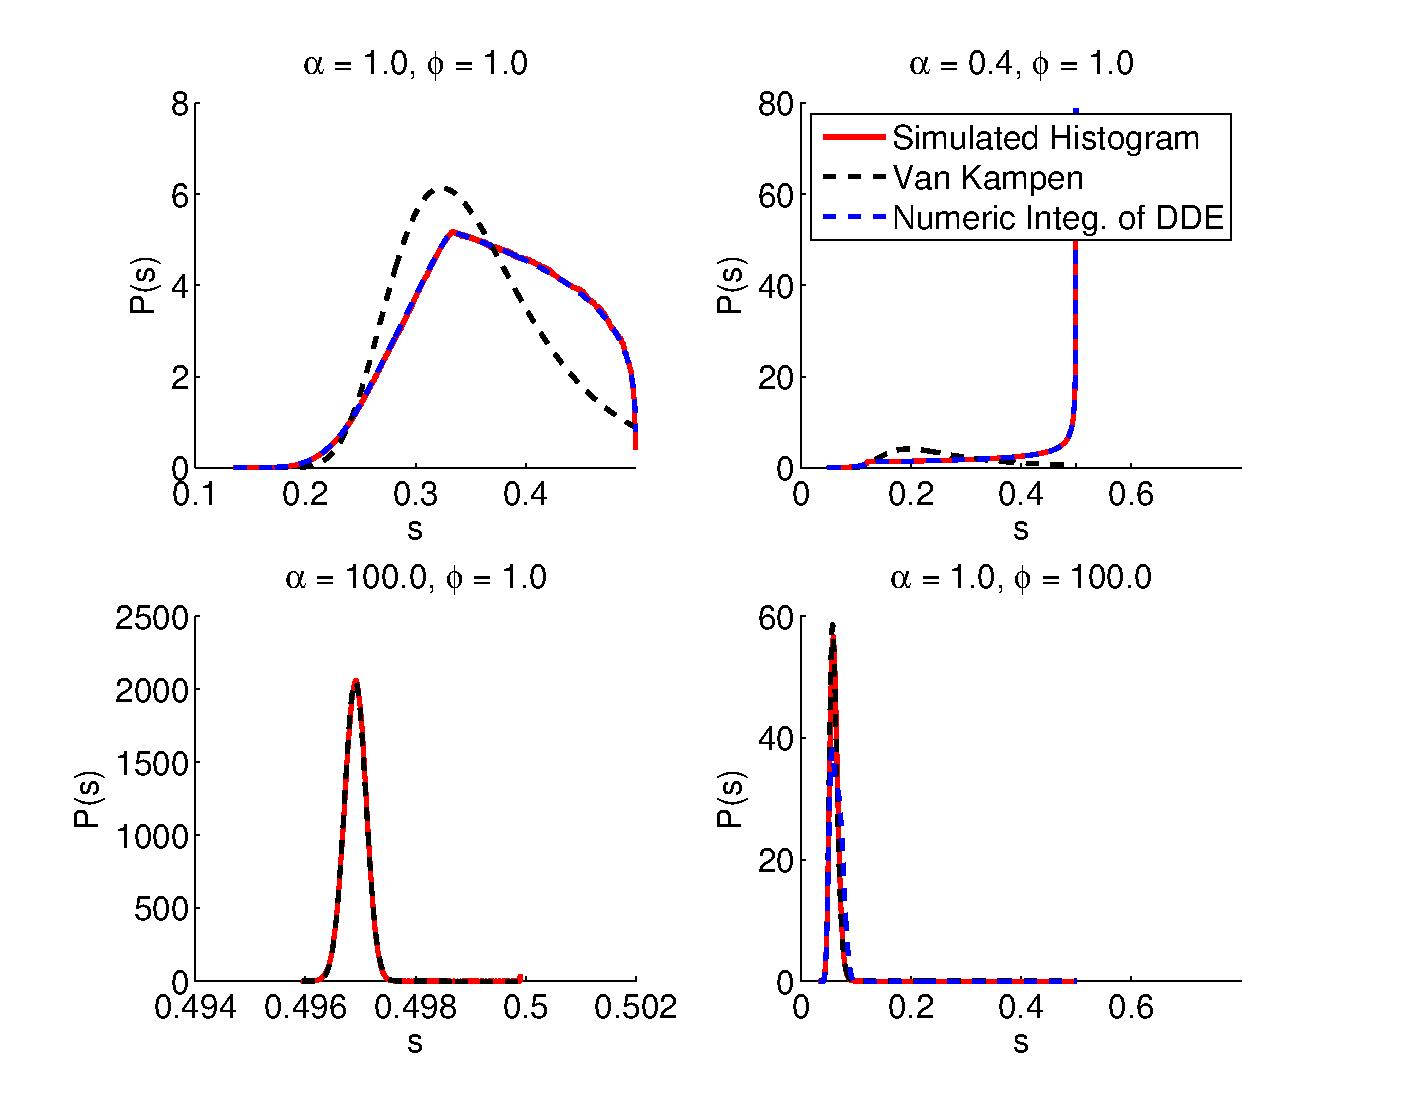
\includegraphics[width=\columnwidth]{figures/figure_3_1.eps}
\caption{The two approaches to solving for the equilibrium distribution described, shown across a range of parameter values.}
\end{figure}
One particularly interesting characteristic of this solution is the exponent. Note that the sign of the exponent in \fref{eq:dist_1d_exact} depends on the specific value of $\hat{\lambda}$ and $2\gamma$. If $\hat{\lambda} > 2\gamma$, the exponent will be larger than 0, leading the distribution to tend to $0$ as $s$ tends to $s_0$. If, however, $\hat{\lambda} < 2\gamma$, the exponent will be negative, leading the distribution to diverge around $s_0$. Notice that $s_0$ is the worst possible performance our encoder can achieve, as it is the variance of the unobserved process. This tells us that whenever the firing rate of the population is below a certain value, the probability distribution of our MSE will be concentrated around its worst possible value. These results are nicely illustrated in \fref{fig:comparison_histograms} where we provide histograms of the exact solution, numerical simulations and a Gaussian approximation to the distribution. This is very interesting, as it relates two different time scales, one ($1/2\gamma$) defines how long information about the observed process stays relevant, while the other ($1/\hat{\lambda}$) given the average time between observations. This provides a rigorous interpretation of an intuitive property of temporal estimation schemes.
\par
Note that, although this result is always valid in the interval $S_0$, we can derive it in the limit of low firing rates as well. If we assume the population firing rate $\hat{\lambda} \ll 2\gamma$, then we will find that the expected interspike interval is much longer than the characteristic time of the variance's dynamics. It is then safe to assume, that whenever a spike is fired, the variance is very close to its equilibrium value $s_0 = \sigma/2\gamma$. The evolution of it after the spike time $t_s$ will then be given by
\[
s(t) = e^{-2\gamma(t-t_s)} s' + s_0 \left(1-e^{-2\gamma (t-t_s)}\right),
\]
where $s' = j(s_0)$,
We can promptly isolate the time in this equation to obtain
\[
\tau \equiv (t-t_s) = -\frac{1}{2\gamma} \log\left(\frac{s_0-s(t)}{s_0-s'}\right).
\]
Clearly, if the spikes are sampled from a Poisson process, then the interspike intervals have a exponential distribution and we will have $P(\tau) \propto e^{-\hat{\lambda}\tau}$. Through a change of variables we then obtain
\[
P(s) = P(\tau) \left|\frac{d\tau}{ds}\right| \propto e^{-\hat{\lambda} \tau + 2\gamma \tau}.
\]
Inserting the definition for $\tau$ we will recover \fref{eq:dist_1d_exact}. Note that this is an approximation for $P(s)$ throughout the range of $s$ for a particular parameter limit, whereas before we had derived an exact result for any parameters, but limited to a small range of values of $s$.\par
We can derive a similar limit for the multidimensional case. Let us first assume $\hat{\lambda}$ is small enough for the covariance $s$ to have relaxed to its equilibrium value $s_0$. After a spike the covariance is then given by $s' = \left(s_0^{-1}+\covar^\dagger\right)^{-1}$. The evolution of $s(t)$ after a spike at $t_s$ is then given by
\[
s(\tau) = e^{\tau G} s' e^{\tau G^\top} + \int_0^\tau e^{\tau G}\sigma e^{\tau G^\top}.
\]
We could in principle proceed as before, but the mapping from the matrix space to the one-dimensional time space can not be explicitly written as above. One alternative is to evaluate the marginals of the diagonal entries of the covariance matrix numerically. We will have, as before,
\[
P(s_{11}) = \frac{P(\tau(s_{11}))}{\left|\frac{d s_{11}}{d\tau}\right|} \propto \frac{e^{-\hat{\lambda} \tau}}{\left|\frac{d s_{11}}{d\tau}\right|}.
\]
We can then evaluate the derivative numerically and obtain an estimate of the distribution of $s_{11}$. If $G$ introduces interactions between the entries of the covariance matrix, however, this result will not prove as powerful, though. As an example, we can consider the Matern processes considered in \citep{Susemihl2012a}, where we have $ds_{11}/dt = s_{12}$. But immediately after the jump, $s'_{12} = 0$, leading the distribution to diverge at $s'_{11}$ as well as in $s^0_{11}$. So, although the divergence around the equilibrium covariance remains, further divergences introduced by the matrix $G$ will reduce the impact of $\hat{\lambda}$ on the shape of the distribution. An example is shown in \fref{fig:matern_histograms}.
\begin{figure}
\label{fig:matern_histograms}
\includegraphics[width=\columnwidth]{figures/matern_histogram.eps}
\caption{The small firing rate limit for the Matern process.}
\end{figure}

\subsection{Van Kampen Approximation}

It is interesting to consider a different approach to gain insight into the behaviour of the distribution of $s$. The Van Kampen approximation consists in linearising
a nonlinear drift function around the equilibrium value of the system and solving the dynamics of the resulting Focker-Planck equation. This is
equivalent to a Gaussian approximation, since a Focker-Planck equation with linear drift always has a Gaussian distribution for a solution. It is simple to apply this
to the OU problem by taking the inverse variance $z= \frac{1}{s}$ instead of the variance.
Note that although the change in the variance when a spike 
is observed is nonlinear, the change in the inverse variance is linear. We have the ODE and jump condition
\[
\frac{dz}{dt} = -\gamma z \left(2- \frac{\eta^2}{\gamma}z\right) \textrm{ and } z(t) = z(t^- ) + \frac{1}{\alpha^2}
\]
for all times $t$ when there is a spike observed. The differential Chapman-Kolmogorov equation for $P(z,t)$ is given by
\begin{equation}
\label{eq:DCKE_Z}
\frac{\partial P(z,t)}{\partial t} = \frac{\partial \left( \gamma z \left(2- \frac{\eta^2}{\gamma}z\right) P(z,t)\right)}{\partial z} + 
\hat{\lambda}\left[ P(z+\frac{1}{\alpha^2},t) - P(z,t)\right].
\end{equation}
The evolution of the average of $z$ is given by
\[
\frac{d\left<z\right>}{dt} = -\gamma\left< z \left(2- \frac{\eta^2}{\gamma}z\right)\right> + \frac{\hat{\lambda}}{\alpha^2},
\]
which gives us the mean-field equilibrium solution of $z^* = \frac{2\gamma}{\eta^2}\left(1+\sqrt{1+\frac{\hat{\lambda} \eta^2}{\gamma^2 \alpha^2}}\right)$. This 
mean-field
approach can be refined by expanding the nonlinear terms in \fref{eq:DCKE_z} around $z^*$ up to second order, which will yield a Focker-Planck equation, which can
be readily solved. The solution to the Focker-Planck equation in the equilibrium will be given by a Gaussian distribution
\[
P_{eq}(z) = \mathcal{N}\left(\frac{2\gamma}{\eta^2}\left(1+\sqrt{1+\frac{\hat{\lambda} \eta^2}{\gamma^2 \alpha^2}}\right), 
\frac{ \hat{\lambda} }{4\alpha^4\gamma \sqrt{1+\frac{\hat{\lambda}\eta^2}{\gamma^2 \alpha^2} }}\right).
\]
This approach is also shown in \fref{fig:comparison_histogram} along with the numerical solution of the delayed-differential equation and the numerical simulations. 
Note that, again, \fref{eq:DCKE_Z} is still exact, and we can look at it to determine when the approximation is appropriate. I have Taylor expanded 
$P(z+\frac{1}{\alpha^2})$ up to second order, and this will yield good approximations whenever $\alpha^2$ is very large. This is seen to be the case in 
\fref{fig:comparison_histogram}, where the Gaussian approximation gives a great account for large values of $\alpha$.

\subsection{Prediction Error}

Note that it also possible to forecast the value of the system's state $X(t)$ into the future. It is relatively simple to do so for the linear stochastic systems described
so far, where one needs simply to integrate the filtering equations further with the observation term set to 0. The MMSE for the prediction is the average covariance
matrix 

\section{A Functional Approach to the MMSE}

Gaussian processes are usually defined in terms of their kernel functions, which give the covariance structure of the process. More precisely for a Gaussian process 
$X(t)$, the kernel gives the covariance between two times $k(s,t) = \left<X(s)X(t)\right>$. I have been able to sidestep the discussion of kernels by considering only
Markov GP's, but one can also develop a theory for the filtering error based on the kernel of the GP directly.\par
In GP regression one is given a set of noisy observations $Y^i$ of $X$ at times $t_i$, with some likelihood function
$P(Y^i|X(t_i))$. This must then be used to infer the distribution over $X(t)$. Generally, one also assumes that the likelihood functions are Gaussian, turning the
inference of $P(X(t)|\{Y^i\})$ into a simple Gaussian marginalisation procedure. This will give us the distribution $P(X(t) | \{Y^i\}) = \mathcal{N}(\mu(t), \Xi(t))$, where
\begin{subequations}
\begin{equation}
\mu(t) = \sum_i k(t,\{t_i\}) C(t_i,t_j) Y^j,
\end{equation}
\begin{equation}
\Xi(t) = k(t,t) - \sum_{i,j}k(t,t_i) C_{ij} k(t_j,t),
\end{equation}
\end{subequations}
where $C = (K+\alpha^2 I)^{-1}$, $K_{ij} = k(t_i,t_j)$ and $\alpha^2$ is the observation noise. Furthermore, note that the covariance of the posterior distribution at two
points is given by
\[
\Xi(s,t) = k(s,t) - \sum_{i,j} k(s,t_i) C_{ij} k(t_j,t).
\]
I will denote the quantity $\Xi(s,t)$ as the posterior kernel, as it again defines a GP. Note that according to the formalism derived so far the MMSE for a filtering 
problem is simply the expected value of the posterior kernel $\Xi(t)$ averaged over the distribution of all possible past observations. Like we have done for the 
MMSE we can look into the dynamics of the posterior kernel $\Xi(s,t)$. Let us write simply $f_t(u,v) = \Xi(t+u,t+v)$, then we have
\[
\frac{\partial f_t(u,v)}{\partial t} = \left( \frac{\partial }{\partial u}+ \frac{\partial }{\partial v}\right) f_t(u,v).
\]
It is a simple exercise in matrix inversion lemmas to show that, if a observation is obtained at time $t$ the posterior kernel will change as
\[
f_t(u,v) = f_{t^-}(u,v) - \frac{f_{t^-}(u,0)f_{t^-}(0,v)}{\alpha^2+ f_{t^-}(0,0)}.
\]
Taking the average over all possible observation paths we obtain the evolution of the average posterior kernel
\[
\frac{\partial \left<f_t(u,v)\right>}{\partial t} = \left( \frac{\partial }{\partial u}+ \frac{\partial }{\partial v}\right) \left<f_t(u,v)\right> - \hat{\lambda} \left<\frac{f_{t}(u,0)f_{t}(0,v)}{\alpha^2+ f_{t}(0,0)}\right>.
\]
Again, we are most interested in the equilibrium case, so setting the derivative to zero we obtain
\begin{equation}
\label{eq:differential_kernel}
\left( \frac{\partial }{\partial u}+ \frac{\partial }{\partial v}\right) \left<f(u,v)\right> = \hat{\lambda} \left<\frac{f(u,0)f(0,v)}{\alpha^2+ f(0,0)}\right>.
\end{equation}
We can now take the mean-field approximation and obtain an integral equation for the average, given by
\begin{equation}
\label{eq:integral_kernel}
\left<f(u,v)\right> = k(u,v) - \frac{\hat{\lambda}}{\alpha^2+ \left<f(0,0)\right>} \int_0^\infty \left<f(s+u,0)\right>\left<f(0,s+v)\right> ds,
\end{equation}
which is easily seen to be a solution to
\[
\left( \frac{\partial }{\partial u}+ \frac{\partial }{\partial v}\right) \left<f(u,v)\right> = \hat{\lambda} \frac{\left<f(u,0)\right>\left<f(0,v)\right>}{\alpha^2+ \left<f(0,0)\right>},
\]
as long as the kernel $k(u,v)$ is stationary, which implies $\partial_u k(u,v) = - \partial_v k(u,v)$. \footnote{A stationary kernel is such that 
$k(t,v) = k(\|t-v\|)$. If $t > v$ and $t> v+d$, then $k(t,v+d) = k(t-d,v)$. Differentiating with respect to $d$ we obtain the desired result.}\par
\Fref{eq:integral_kernel} allows us to approximate the shape of the posterior kernel directly from the prior kernel, without having to resort to the Markovian structure of
the process as had been done before. This is very practical as it allows us to treat non-Markovian GP's such as the one defined by the squared exponential or Radial
Basis Function kernel.\footnote{The SE or RBF kernel is given by $k(t,v) = c \exp(-\|t-v\|^2/L^2)$.} This can still be done only for the Mean-field approximation, but it is
still a very pleasing result, as it additionally allows us to estimate the shape of the entire posterior kernel, not only of the one-time variance. If we are only interested
in the filtering error however, it suffices to take the function $g(u) = \left<f(u,0)\right>$. For that the equation simplifies to
\begin{equation}
\label{eq:integral_one_point}
g(u) = k(u,0)  - \frac{\hat{\lambda}}{\alpha^2+ g(0)} \int_0^\infty g(s+u)g(s) ds
\end{equation}
One way to solve \fref{eq:integral_kernel} is to simply discretise the real line over some interval $[0,D]$ and iterate \fref{eq:integral_one_point} numerically. A reasonable
initial condition would be to take $g^0(u) = k(u,0)$ and then simply take
\[
g^{i+1}(u) = k(u,0)- \frac{\hat{\lambda}}{\alpha^2+ g^i(0)} \int_0^\infty g^i(s+u)g^i(s) ds.
\]
This is shown in \fref{fig:integral_kernel} for the OU kernel $k_{OU}(s,t) = \exp(-k|s-t|)$, for the Matern kernel $k_{mat}(s,t) = (1+k|t-s|) \exp(-k|t-s|)$ and the 
RBF kernel $k_{dbf} = \exp(-k|t-s|^2)$. Note that once we have have an approximation for $g(u)$ we can in principle approximate the posterior average of the kernel
at all points by repeating the procedure. From \fref{eq:integral_kernel} we can see that $\left<f(u,v)\right>$ is only a function of $\left<f(t,0)\right>$ and 
$\left<f(0,s)\right>$, both of which we can approximate with $g$.
\begin{figure}
\label{fig:}
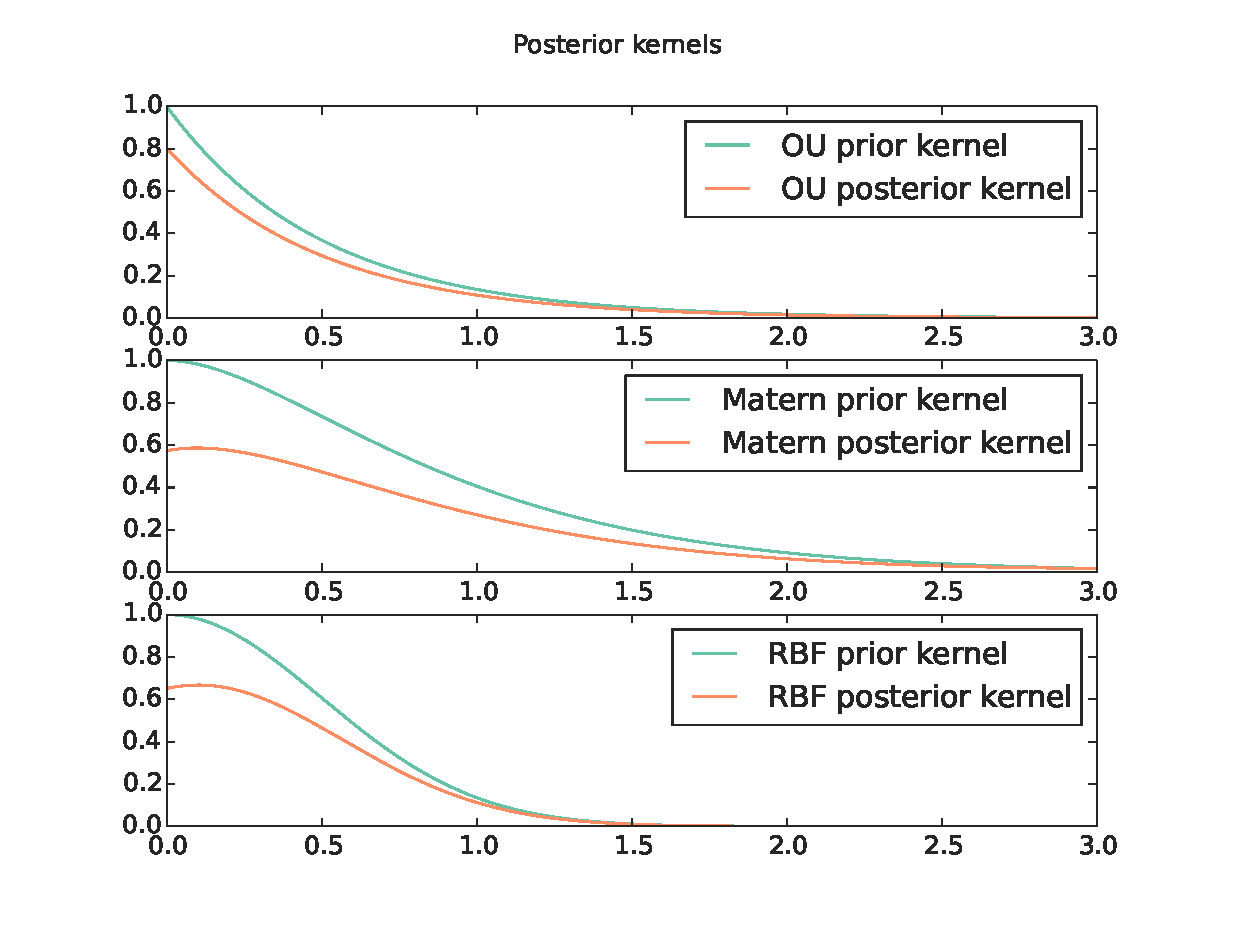
\includegraphics[width=\columnwidth]{figures/figure_3_3.eps}
\caption{The prior and posterior kernels for the filtering problem for three classes of GP's.}
\end{figure}



\chapter{Optimal Control with Point Process Observations}

\label{chap:control}

\newthought{Clearly the nervous system is not solely interested in estimating the state of the world.} Furthermore, if that estimate is not useful for making decisions and taking actions 
in a dynamic environment, there is little use for it. In the previous chapter I have discussed findings for spiking codes in an estimation context. In this chapter I will extend this approach 
to the framework of stochastic optimal control, and discuss how to reframe the findings in this context.\par

The field of optimal control has been of growing interest to the neuroscience community, but little attention has been given to the issue of optimal coding in a control context. Here I
will study a simple case of linear quadratic control observed through a dense population of Gauss-Poisson neurons, for which I have been able to derive a closed-form expression
for the optimal cost-to-go. This allows one to study the expected control cost in an experiment as a function of the encoder, similarly to what I have done with the MMSE in the previous 
chapters. Furthermore, in \fref{chap:optimal} I will compare these two approaches, showing that in a couple of simple examples, the control-optimal and the MMSE-optimal encoders
differ significantly.

\section{Optimal Control}
The field of control theory is concerned with the steering and controlling of systems, always with the minimization of a cost (or maximization of a reward) in mind. Speaking mathematically, given a system with state $X(t) \in \mathcal{X}$, with dynamics given by
$$
\dot{X}(t) = f(X(t),U(t)), \quad X(0) = x_0
$$
one would like to select the control variables $U(t) \in \mathcal{U}$ in such a way as to minimize an integrated cost function over time\footnote{This is an additive cost function,
which is itself only a specific kind of control problem. Generally one can also consider more complex cost functions as well, that depend on the minimum or maximum
of the state or multiplicative cost functions.}
$$
C(X_{0:T},U_{0:T}) = \int_{0}^T c(X(s),U(s),s) ds + h(X(T)).
$$
Here $c(x,u,t)$ specifies a cost rate accumulated over time and $h(x)$ describes some final goal the system should achieve at the end of the control problem.\par

In a purely deterministic setting, the solution to the control problem would be a policy $U^* : \mathcal{X} \times \mathbf{R}\to \mathcal{U}$ which for each system 
state and time gives a control to be applied to the system when it is in that state at that time. One would have\marginnote{The minimum of the future cost over the space of controls is called the value function $V(X,t)$.}
$$
\min_{U_{0:T}} C(X_{0:t},U_{0:t},0;x_0) = C\left(X_{0:t},U^*(X_{0:t}),0\right) \equiv V(x_0,0),
$$
where $V(x,t)$ is usually called the optimal cost-to-go function or the value function. $V(x,t)$ quantifies the cost one is expected to incur if he controls the system optimally through the 
remainder of the control problem, given that the system is at state $X(t)=x$ at time $t$.\par

This is a very broad formulation, but one general remark can be made, though, first put forward by Richard Bellman.\mycite{Bellman1952} Bellman 
proposed an optimality principle\marginnote{Bellman's principle of optimality}, which stated that if a given policy is an optimal solution to a control problem, then the 
policy resulting after a number of steps of that policy must still be optimal for the remaining control problem as well. This can be formulated as a mathematical equation, 
the so-called Bellman equation or dynamic programming equation, which states that the minimal future cost in state $X(t)$ at time $t$ is given by the minimum over 
$U(t)$ of the instantaneous cost plus the minimal future cost at the resulting future state $X({t+dt})$. Mathematically, we have
\begin{equation}
\label{eq:bellman_eq}
V(X(t),t) = \min_{U(t)} \left[ c(X(t),U(t),t) dt +V(X({t+dt}),t+dt)\right].
\end{equation}
Note that in general, $X({t+dt})$ will depend on $U(t)$, making the solution of the Bellman equation difficult.\par
In continuous time, assuming differentiability of the value function $V$ in both its, one obtains
\[
V(X(t),t) = \min_{U(t)} \left[c(X(t),U(t),t) dt + V(X(t),t) + \frac{\partial V}{\partial t} dt + \frac{\partial V}{\partial x} dX(t) \right],
\]
which leads to the Hamilton-Jacobi-Bellman equation\marginnote{I will abbreviate the Hamilton-Jacobi-Bellman equation as HJB equation.}
$$
-\frac{\partial V}{\partial t} = \min_{U(t)} \left[c(x,U(t),t) + \frac{\partial V}{\partial X} f(x,U(t)) \right].
$$
This is often more convenient to solve, as it sometimes allows for explicit minimisation over the control. The HJB equation must be solved backwards in time, with final condition $V(x,T) = h(x)$.

\subsection{Estimation and the Separation Principle}

In the previous two chapters, I have considered the problem of filtering a stochastic process from spike trains. More specifically, given a signal, I was looking for the optimal set of 
parameters $\varphi^*$ for a population of neurons that minimise the MMSE of the filtering problem. Here I would like to establish a similar approach to control problems. That is,
in the same sense of before, I have a noisy system observed through spike trains of a population of neurons specified by some parameters $\varphi$, but now I am concerned with
controlling this noisy system. Given a cost function, I would like to determine the parameters $\varphi^*$ that minimise the control costs, instead of the filtering error.
If one is interested in controlling a system, say a limb performing a movement, one must now deal with the uncertainties in the system and control it according to noisy estimates of its 
state. The certainty equivalence property (CEP) holds if a system one only has partial information about can be controlled ignoring the uncertainty in its state and acting as if it were 
fully observed. I will elaborate below.
\par

Consider a deterministic system
\[
\dot{X} = f(X(t),U(t)),
\]
where I have only partial knowledge about the system's state through an initial distribution $P_0(x)$ and noisy observations $Y(t)$ of the system's state. If the certainty 
equivalence property holds for this system, the optimal control for the partially-observed system, will be the optimal policy of the fully observed problem applied to the mean estimate
of the system's state. To be more precise, let me define the cost for the partially-observed system as
\[
C(P_0,Y_{0:T},U,0) = \int_0^T \boldsymbol{E}  \left[c(X(s),U(s),s) \mid Y_{0:s},P_0 \right]ds + \boldsymbol{E} \left[h(X(T))\mid Y_{0:T},P_0\right].
\]
The optimal control $U^*$ will now be a function of the observations $Y_{0:t}$ up to time $t$ and the initial distribution $P_0$. If the optimal control for the fully-observed system is 
given by $U^*_{obs}(x,t)$, the certainty equivalence property holds if the optimal control for the partially observable process is given by 
$$
U^*_{part} (Y_{0:t},P_0,t) =  U^*_{obs}\left(\boldsymbol{E}\left[X(t) \mid Y_{0:t},P_0\right],t\right).
$$
This means that the uncertainty in the system's state can be treated in two independent steps, first estimating the system's state through the posterior mean and then applying the
control as if our estimate of the state was certain. Hence the name certainty equivalence, as one applies the control as if they were certain about the system's state.
The separation property is also frequently discussed in the literature, and it is a stronger version of the certainty equivalence property, where the control $U^*_{obs}(x,t)$ being 
employed does not need
to be the optimal policy for the fully observed problem, but can be related to some other control problem with full informations.\par

One can now ask what is the encoder that minimises the expected control costs. It is tempting to conclude from the CEP that the encoder that minimises the MMSE also minimises
the control costs. This is not true, however, as I will show in \fref{chap:optimal}. I will now consider the case of stochastic optimal control, and then turn to the case of 
partially-observable stochastic optimal control. This can be treated for the case of dense Gauss-Poisson observations, and I will derive a novel relation for the optimal cost-to-go
for that case.

\section{Stochastic Optimal Control}

The world is a noisy place, and if to control real-world systems, one must be able to account for noise in the systems as well. One simple way to include noise is to generalise the system dynamics to a stochastic differential equation. Consider
$$
dX(t) = f(X(t),U(t)) dt + H^{1/2} dW(t),
$$
where $W(t)$ is a standard Wiener process. It is not possible to predict the evolution of $X(t)$ exactly anymore, so one must redefine the cost function. The natural way
to do so is to define it as the average over future states conditioned on the current state $X(t)$ and the controls to be applied $U(t)$. This will lead to
\[
C(X,U) = \boldsymbol{E} \left[\int_0^T c(X(t),U(t),t) dt \biggm\vert X(0), U_{0:T}\right].
\]
One should mention that there are other ways to deal with the stochastic nature of the problem, such as the risk-sensitive control approach,\mycite{whittle1981} where one considers
the cost function
\[
C_{\theta}(X,U) = \frac{1}{\theta} \log \boldsymbol{E} \left[\exp\left(-\theta \left(\int_0^T c(X(t),U(t),t) dt + h(X(T))\right)\right)\right].
\]
In the limit $\theta\to 0$ one recovers the former formalism. This allows one to consider risk-averse or risk-seeking control policies. I will not, however, consider this approach here.\par
The Bellman equation can then be extended to the stochastic case as
\begin{equation}
\label{eq:stochastic_bellman}
V(x,t) = \min_{U(t)}\boldsymbol{E}\left[ c\left(X(t),U(t),t\right) dt + V\left(X(t+dt),t+dt\right)\mid\,X(t)=x, U_{[t,T]}\right].
\end{equation}
Using It\=o's lemma for the variation of $V$, and averaging over the Brownian motion $dW(t)$ leads to
\[
V(x,t) = \min_{U(t)} \left[ c(x,U(t),t) dt + V\left(x,t\right)+\left(\frac{\partial V}{\partial t} dt + f(x,U(t))^\top \frac{\partial V}{\partial x} +\frac{1}{2} \Tr\left[H \frac{\partial^2 V}{\partial x^2} \right]\right)dt \right].
\]
This leads to the stochastic HJB equation
\begin{equation}
\label{eq:stochastic_HJB}
-\frac{\partial V}{\partial t} = \frac{1}{2} \Tr\left[H \frac{\partial^2 V}{\partial x^2} \right] +\min_{u} \left[ c(x,u,t)  + f(x,u)^\top \frac{\partial V}{\partial x}\right].
\end{equation}
\par
One could also consider a Poisson process as a noise source. If one takes, for example, a Poisson counting process $N(t)$, with time- and/or
 state-dependent rate $\lambda(X(t),t)$, and takes the system dynamics to be given by a drift-diffusion process with state-dependent jumps $j(X(t),t)$, occurring with
 rate $\lambda(X(t),t)$ then the SDE for the state would be,
$$
dX(t) = f(X(t),U(t)) dt + H^{1/2} dW(t) + j(X(t),t) dN(t).
$$
This would lead to the full HJB equation for a drift-jump-diffusion process controlled by some control process $U(t)$
\begin{equation}
\label{eq:martingale_HJB}
-\frac{\partial V}{\partial t} = \min_{u} \left[c(x,u,t) + f(x,u)^\top \frac{\partial V}{\partial x} + \frac{1}{2} \Tr\left[H \frac{\partial^2 V}{\partial x^2} \right] + \lambda(x,t) \left[V(x+j(x,t),t)-V(x,t)\right]\right],
\end{equation}
now including the terms regarding the jump process.\mycite{Theodorou2012,Sennewald2006} Note that the statistics of the posterior distribution of the filtering problem from the previous
chapters fit this description, namely they are a jump-drift processes with no diffusion. I will use this formalism to derive a belief state formulation of a control problem with dense
Gauss-Poisson observations.

\subsection{Linear-Quadratic-Gaussian Control}

The Linear-Quadratic-Gaussian\footnote{LQG} control problem is defined by linear dynamics in both the state and the control variable, a quadratic cost rate function
$c$ in both the state and control and a Gaussian noise source. I will treat this problem here to illustrate the optimal control formalism.
This would mean that the evolution of the state is given by the SDE
\begin{equation}
\label{eq:ctl_diff_dyn}
dX(t) = \left(A X(t) + B U(t)\right) dt + H^{1/2} dW(t),
\end{equation}
where $W(t)$ is a Wiener process. Taking a cost rate given by
$$
c(X(t),U(t),t) = U(t)^\top R(t) U(t)+ X(t)^\top Q(t) X(t),
$$
and a final cost given by $h(X(T)) = X(T)^\top Q_T X(T)$, one can solve for the value function explicitly, using the HJB equation. The HJB equation in this case will be given by
$$
-\frac{\partial V}{\partial t} = \min_{U(t)} \left[ U(t)^\top R(t) U(t) +  x^\top Q(t) x + \frac{\partial V}{\partial x}^\top \left(A x  + B U(t)\right) + \frac{1}{2} \Tr\left(H\frac{\partial^2 V}{\partial x^2}\right) \right].
$$
One can minimize the right hand side explicitly and eliminate $U$ from the equation. One obtains that the optimal control is given by
$$
U^*(x,t) = -\frac{1}{2} R(t)^{-1} B^\top\frac{\partial V}{\partial x}\big|_{x,t}.
$$
Inserting into the HJB equation once more leads to
\begin{equation}
\label{eq:lqg_hjb}
-\frac{\partial V}{\partial t} = x^\top Q(t) x +\frac{\partial V}{\partial x}^\top A x -\frac{\partial V}{\partial x}^\top B R(t)^{-1} B^\top \frac{\partial V}{\partial x} + \frac{1}{2}\Tr\left(H\frac{\partial^2 V}{\partial x^2}\right).
\end{equation}
It can be shown that $V$ can only have a quadratic dependence in $X$, since at the final time the cost is given by $h(X(N))$ which is quadratic, and the HJB equation will preserve
this property. I will assume it is of the form $V(x,t) = x^\top S(t) x + \alpha(t)^\top x + k(t)$. Inserting this into \fref{eq:lqg_hjb}
gives the ODE's for the parameters of the value function
$$
-\dot{S} = Q(t) + A^\top S(t) + S(t) A - S(t) B R(t)^{-1} B S(t),
$$
$$
-\dot{\alpha} = A^\top \alpha(t)-S(t) B R(t)^{-1} B^\top \alpha(t),
$$
$$
-\dot{k} = \Tr\left(H S(t)\right)-\alpha(t)^\top B R(t)^{-1} B^\top \alpha(t),
$$
with the terminal conditions $S(T) = Q_T$, $\alpha(T) = 0$ and $k(T)=0$. The $X$-independent term $k(t)$ accounts for the future uncertainty in $X$, decreasing to $0$ over time as we approach the final time $T$. Furthermore, the differential equation for $S(t)$ is a special case of the Riccati equation. The full optimal control for the LQG control problem will 
therefore be given by
\[
U^*(x,t) = -R(t)^{-1}B^\top S(t) x.
\]

These results can also be extended to the case of control- and state-dependent diffusion noise, affine dynamics and some other cases.\mycite{Kappen2011}

\section{Partially Observable Processes}

In general, one does not have access to the exact state of the system, and it is useful to consider cases where one is only given noisy observations of the state, as were considered in 
the previous chapters. The most commonly considered case of partially observable control problem is a LQG problem observed through a second diffusion process. Suppose one has 
as above a system $X(t)$ evolving according to \fref{eq:ctl_diff_dyn}, but instead of observing $X(t)$ directly, one observes the process $Y(t)$, which I shall call the 
observation process, given by
\begin{equation}
\label{eqn:ctl_obs_dyn}
dY(t) = C X(t) dt + D^{1/2} dV(t).
\end{equation}
Given a control trajectory $\{U(s), s\in [0,t]\}$, the problem of estimating $X(t)$ given observations ${Y(s), s \in [0,t]}$, is a simple filtering problem, and is solved exactly by the Kalman-Bucy filter.\footnote{See \fref{chap:filtering}.} It will lead to a Gaussian estimate of $X(t)$ with mean $\mu(t)$ and variance $\Sigma(t)$, where $\mu$ and $\Sigma$ evolve according to
\begin{subequations}
\label{eq:ctl_kalman_bucy}
\begin{equation}
d\mu(t) = (A \mu(t) + B U(t))dt + \Sigma(t) C^t D^{-1} \left(dY(t) - C\mu(t) dt\right),
\label{eq:ctl_kalman_bucy_mean}
\end{equation}
and
\begin{equation}
\label{eq:ctl_kalman_bucy_var}
\frac{d\Sigma}{dt} = A \Sigma + \Sigma A^\top + H - \Sigma C^\top D^{-1} C \Sigma.
\end{equation}
\end{subequations}
Since in this case we do not have perfect information on the process to be controlled, we have to settle for the goal of minimizing the expected cost given our observation. Therefore, the cost to be minimized is
$$
C(U_{0:T};\mu_0,\Sigma_0) = \boldsymbol{E}\left[\int_{t_0}^T c(X(t),U(t),t)dt +h(X(t))\right],
$$
where the average is over all future paths of $X(t)$ and all observation paths $Y(t)$.
There is no analogous to the HJB equation for the incomplete information case, but I will reformulate the problem as a control problem over the belief states, that is, the state of the world as one is led to believe it is distributed given the previous observations\marginnote{The belief state is a description of an system with incomplete information which eschews describing the actual state of the system, instead describing the distribution over states. A general formulation is described in \mycitep{bertsekas2012}.}. In the case I am discussing, the belief state is the distribution over the state variable, given by the Gaussian distribution $\mathcal{N}(\mu(t),\Sigma(t))$. The dynamics of the belief state is then given by equations \fref{eq:ctl_kalman_bucy_mean} and \fref{eq:ctl_kalman_bucy_var}. Note that when one chooses to describe the system in terms of the mean and variance of the posterior distribution, the noise process $dW(t)$ does not enter into the analysis anymore, and the observation process $dY(t)$ takes the role of the noise process. We need, however, to redefine the cost function $c(X(t),U(t),t)$ to fully specify the problem. The average cost is
$$
\boldsymbol{E}\left[c(X(t),U(t),t)\middle|\mu(t),\Sigma(t) \right] = U(t)^\top R(t) U(t) +\left(\mu(t)^\top Q(t) \mu(t) + \Tr\left(Q(t)\Sigma(t)\right)\right),
$$
from which one can define a belief-state cost rate, which makes no mention of the underlying unobservable process
\[
c(\mu,\Sigma,U,t) =  U(t)^\top R(t) U(t) +\mu(t)^\top Q(t) \mu(t) + \Tr\left(Q(t)\Sigma(t)\right).
\]
One can now write the HJB equation for the system described by \fref{eq:ctl_kalman_bucy}, leading to
$$
V(\mu(t),\Sigma(t),t) = \min_{U(t)} \boldsymbol{E}\left[ U(t)^\top R(t) U(t)+\left(\mu(t)^\top Q(t) \mu(t) + \Tr\left(Q(t)\Sigma(t)\right)\right)+V(\mu(t+dt),\Sigma(t+dt),t+dt)\right],
$$
where the expectation is now with respect to the observation process $Y(t)$.
Taking the variation of $V$ with infinitesimal time increments via It\=o's lemma one has
$$
dV = \frac{\partial V}{\partial t} dt + \frac{\partial V}{\partial \mu}^\top d\mu + \Tr\left[\frac{\partial V}{\partial \Sigma}d\Sigma\right] +\frac{1}{2} \Tr\left[(\Sigma C^\top D^{-1} C 
\Sigma)_{i,j} \frac{\partial^2 V}{\partial \mu^2}\right],
$$
which leads to the HJB equation
\begin{eqnarray*}
-\pd{V}{t} =& \min_{U(t)} \boldsymbol{E}\left[ U(t)^\top R(t) U(t)+\mu(t)^\top Q(t) \mu(t) + \Tr\left(Q(t)\Sigma(t)\right) +\frac{\partial V}{\partial \mu}d\mu^\top\right] \\&+ \Tr\left[\frac{\partial V}{\partial \Sigma}d\Sigma\right] +\frac{1}{2} \Tr\left[(\Sigma C^\top D^{-1} C \Sigma)_{i,j} \frac{\partial^2 V}{\partial \mu^2}\right] .
\end{eqnarray*}
Minimization with respect to $U(t)$ leads to $U^*(t) = -R(t)^{-1} B^\top \pd{V}{\mu}$, which results in
\begin{eqnarray}
-\pd{V}{t} =& \mu^\top Q(t)\mu + \pd{V}{\mu}^\top B R(t) B^\top \pd{V}{\mu} + \Tr\left(Q(t)\Sigma(t)\right) +\frac{\partial V}{\partial \mu}d\mu^\top\nonumber\\&+ \Tr\left[\frac{\partial V}{\partial \Sigma}d\Sigma\right] +\frac{1}{2} \Tr\left[(\Sigma C^\top D^{-1} C \Sigma)_{i,j} \frac{\partial^2 V}{\partial \mu^2}\right] .
\label{eq:lqg_hjb_partial}
\end{eqnarray}
This would now have to be solved backwards from $V(\mu,\Sigma,T) = \mu^\top Q_T \mu + \Tr[\Sigma Q_T]$. \Fref{eq:lqg_hjb_partial} provides a clean formulation of the control problem in 
terms of the belief state, where the underlying process has been integrated over completely. This is a very useful approach and I will leverage it for the case of Point processes
observations below.
If I write the value function as $V(\mu,\Sigma,t) = \mu^\top S(t) \mu + f(\Sigma,t)$, I will obtain the same Riccati equation for $S(t)$ as in the fully observed case. Using this form for
the value function, one immediately recovers the optimal control $U^*(t) = -R^{-1}(t) B^\top S(t) \mu$, which shows the certainty equivalence property for this system.
\section{Partially Observable Processes with Poisson Observations}

Similarly to the case just discussed, we can consider the case of a stochastic system observed through a population of densely tuned Poisson processes with Gaussian tuning functions. The dynamics of the system would be the same as \fref{eq:ctl_diff_dyn}, but the observation processes would be given by a set of $M$ Poisson processes $N^m$ with rates given by
\begin{equation}
\label{eq:ctl_poisson_rate}
\lambda^m(X(t)) = \lambda \exp\left[-\frac{1}{2}(\theta_m-X(t))^\top \covar^\dagger (\theta_m-X(t))\right],
\end{equation}
where the tuning centres $\theta_m$ are positioned in such a way that the overall firing rate of the population $\hat{\lambda} = \sum_m \lambda^m(X(t))$ is independent of the system's
state $X(t)$.
As we have shown in \fref{chap:filtering}, the estimation problem is solved by the point-process analog of the Kalman-Bucy filter, first derived by Donald Snyder.\mycite{Snyder1972,Bobrowski2009} In the present case, with Gaussian tuning functions, the filtering equations are
\begin{subequations}
\begin{eqnarray}
d\mu(t) =& (A\mu(t) + B X(t)) dt \nonumber\\
+& \sum_i  \left[\Sigma(t^-)\left(I+\covar^\dagger \Sigma(t^-)\right)^{-1} \covar^\dagger\left(\theta_i - \mu(t^-)\right)\right]dN^i(t)\nonumber\\ 
\label{eq:ctl_poisson_mean}
\end{eqnarray}
and
\begin{eqnarray}
d\Sigma(t) =&\left(A\Sigma(t) + \Sigma(t) A^\top + H\right)dt\nonumber \\
-&  \left[\Sigma(t^-) \covar^\dagger \Sigma(t^-) \left(I+\covar^\dagger \Sigma(t^-)\right)^{-1}\right] dN(t),
\label{eq:ctl_poisson_var}
\end{eqnarray}
\end{subequations}

where $dN(t) = \sum_m dN^m(t)$. I will define 
$$
\delta \mu(t) \equiv (A\mu(t) + B X(t)) dt
$$
as the continuous part of $d\mu(t)$ and 
$$
\Delta^i \mu(t) \equiv dN^i(t) \left[\Sigma(t^-)\left(I+\covar^\dagger \Sigma(t^-)\right)^{-1} \covar^\dagger\left(\theta_i - \mu(t^-)\right)\right]
$$
as the jump part of $d\mu(t)$. Likewise, for the variance, define
$$
\delta\Sigma(t) \equiv (A\Sigma(t) + \Sigma(t) A^\top + H)dt
$$ 
and
$$
\Delta\Sigma(t) \equiv dN(t) \left[\Sigma(t^-) \covar^\dagger \Sigma(t^-) \left(I+\covar^\dagger \Sigma(t^-)\right)^{-1}\right].
$$\par
These give the evolution of the optimal Bayesian filter, with the posterior distribution over $X(t)$ conditioned on the observations $\{N^m(s), m\in [1,\ldots,M], s\in[t_0,t]\}$,
given by the normal distribution $\mathcal{N}(X(t);\mu(t),\Sigma(t))$. Assuming one is trying to minimize a cost given by the same cost rate $c(X(t),U(t),t)$ as before, one canwrite out 
the infinitesimal Bellman equation for this case as well. Since the dynamics of the system and the observations is Markov, I can use the posterior distribution as a sufficient statistic for 
the knowledge of the system's state. I will therefore take the belief state to be the mean and variance of the posterior distribution as before.\footnote{See \mycitep{bertsekas2012} for a 
more  detailed discussion.}
Similarly to the previous sections, I will consider the processes $N^m(s), s\le t$ as noise to be averaged over in the future. This leads to
$$
V(\mu(t),\Sigma(t),t)= \min_{U(t)} \left\{\boldsymbol{E}_{X(t)}\left[c(X(t),U(t),t)\right] + \boldsymbol{E}_{\{N^m(t)\}}\left[V(\mu({t+dt}),\Sigma(t+dt),t+dt)\right]\right\}
$$
According to It\=o's lemma, one obtains
\begin{eqnarray*}
V(\mu({t+dt}),\Sigma(t+dt),t+dt) =& V(\mu(t),\Sigma(t),t) + \frac{\partial V}{\partial t}dt + \frac{\partial V}{\partial \mu} \delta\mu(t) +\Tr\left[\frac{\partial V}{\partial \Sigma} \delta \Sigma(t)\right]\\ &+ \sum_m dN^m(t)\left[V\left(\mu(t) +\Delta^m\mu(t) , \Sigma(t)+\Delta\Sigma(t),t\right)-V(\mu(t),\Sigma(t),t)\right].
\end{eqnarray*}
The expectation over the noise process $N^m(t)$ in the Bellman equation can then be written as
\begin{eqnarray*}
\boldsymbol{E}(V_{t+dt})_{N^m(t)} =&V(t) + \frac{\partial V}{\partial t}dt + \frac{\partial V}{\partial \mu} \delta\mu(t) +\Tr\left[\frac{\partial V}{\partial \Sigma} \delta \Sigma(t)\right]\\ +& \sum_m \boldsymbol{E}_{N^m(t)}\left[dN^m(t)\left[V\left(\mu(t) +\Delta^m\mu(t) , \Sigma(t)+\Delta\Sigma(t),t\right)-V(\mu(t),\Sigma(t),t)\right]\right] \\
 =&V(t) + \frac{\partial V}{\partial t}dt + \frac{\partial V}{\partial \mu}^\top \delta\mu(t) +\Tr\left[\frac{\partial V}{\partial \Sigma} \delta \Sigma\right]\\ +& \sum_m \boldsymbol{E}_{X(t)}[\lambda^m(X(t))] \left[V\left(\mu(t) +\Delta^m\mu(t) , \Sigma(t)+\Delta\Sigma(t),t\right)-V(\mu(t),\Sigma(t),t)\right],
\end{eqnarray*}
leading to the HJB equation
\begin{eqnarray}
-\frac{\partial V}{\partial t} &=\mu^\top Q(t)\mu + \Tr\left(Q(t) \Sigma\right) +(U(t))^\top R(t) U(t)  + \frac{\partial V}{\partial \mu}^\top \delta\mu +\Tr\left[\frac{\partial V}{\partial \Sigma} \delta \Sigma\right] \\
&+\sum_m \boldsymbol{E}_{X(t)}\left[\lambda^m(X(t))\right]\left[V\left(\mu(t) +\Delta^m\mu(t) , \Sigma(t)+\Delta\Sigma(t),t\right)-V(\mu(t),\Sigma(t),t)\right]\nonumber.
\end{eqnarray}
Minimisation with respect to the control, gives us the optimal control policy
\[
U^*(t) = -R(t)^{-1} B^\top \frac{\partial V}{\partial \mu}\bigg|_{\mu=\mu(t),\Sigma=\Sigma(t)}.
\]
This yields
\begin{eqnarray}
-\frac{\partial V}{\partial t} =&\mu^\top Q(t)\mu + \Tr\left(Q(t) \Sigma\right) - \frac{\partial V}{\partial \mu}^\top B R(t)^{-1} B^\top \frac{\partial V}{\partial \mu}  + \frac{\partial V}{\partial \mu} A \mu  \\
&+\Tr\left[\frac{\partial V}{\partial \Sigma} \delta \Sigma\right]+\sum_m \boldsymbol{E}_{X(t)}\left[\lambda^m(X(t))\right] \left[V\left(\mu(t) +\Delta^m\mu(t) , \Sigma(t)+\Delta\Sigma(t),t\right)-V(\mu(t),\Sigma(t),t)\right]\nonumber.
\end{eqnarray}
It can be shown that the optimal cost-to-go function is of form $V(\mu,\Sigma,t) = \mu^\top S(t) \mu + f(\Sigma,t)$, since it is of this form at the final time $T$ because 
of the final cost $h(x) = x^\top Q_T x$. I can now write down the equations for $S(t)$ and $f(\Sigma,t)$. The equation for $S(t)$ is the same as for 
the LQG case
\begin{equation}
\label{eq:riccatti}
-\dot{S}(t) = Q(t) - S(t) b R(t)^{-1} b^\top S(t) + S(t) a + a^\top S(t).
\end{equation}
The equation for $f(\Sigma,t)$ can be shown to be\footnote{See \fref{app:f_sigma}.}
\begin{equation}
-\frac{\partial f}{\partial t} = \Tr\left(Q(t) \Sigma\right) + \frac{\partial f}{\partial \Sigma} \left(A\Sigma + \Sigma A^\top + H\right) + \hat{\lambda} \left[f(\Sigma+\Delta\Sigma,t) - f(\Sigma,t) + \Tr\left(\Sigma S(t) \Sigma \left(\Sigma+\covar\right)^{-1}\right)\right].
\label{eq:f_variance}
\end{equation}
\Fref{eq:f_variance} gives the contribution of the uncertainty of the estimate to the future costs. This allows one to quantify the effect of our encoder on the control costs. In
\fref{chap:optimal} I will use $f$ to determine the optimal encoding strategies for a simple control problem. \Fref{eq:f_variance} can be shown to be solved by
\begin{equation}
\label{eq:poiss_cost}
f(\Sigma,t)  = \Tr\left(\Sigma(t) S(t)\right) + \int_t^T \Tr\left(H S(u)\right)du+ \int_t^T \Tr \left(S(u) B^\top R(u)^{-1}B S(u) \boldsymbol{E}\left[\Sigma(u)\mid \Sigma(t) = \Sigma \right]\right) du.
\end{equation}
where the expectation is over all paths of \fref{eq:ctl_poisson_var} with initial condition $\Sigma(t) = \Sigma$. I provide a derivation of this result based on the Feynman-Kac formula in
\fref{app:feynman_kac}.
This equation allows one to separate the different ways in which the uncertainty affects the expected future cost. The first term accounts for the uncertainty in the present estimate
of the system's state. The second term is due to the stochastic nature of the stimulus $X(t)$, and describes the accumulation of uncertainty due to the Brownian noise in that process. 
The third term accounts for the effect of the uncertainty on the applied control. If one is uncertain of the system's state, the control applied will not be exactly the optimal for the system's 
state, and additional costs will be incurred because of that. The third term is also the only one that depends on the parameters of the encoder, more specifically it depends on the
future dynamics of the posterior covariance $\Sigma(t)$, which in turn depends on the firing rates and the tuning widths. A similar relation can be derived for the LQG case as 
well,\footnote{See \citep[p. 290]{astrom2006} for the full derivation.} but
the full result for the partially observable control with Point process observations is novel.
\par

From the derivation above, it follows that the optimal control is again given by
\[
U^*(t) = -R(t)^{-1} B^\top S(t) \mu(t),
\]
showing that the certainty equivalence property holds in this case as well. I will discuss these issues further in \fref{sec:optimal_code_control}.\par
The finding that the certainty equivalence
property holds in this simple set up, along with the exact expression for the optimal cost-to-go has not been shown in the literature to the best of my knowledge, and I believe it to
provide a good starting point for the study of optimal codes in a control-theoretical setting.


%
%Below I will derive a Feynman-Kac formulation to solve for the uncertainty-related cost $f(\Sigma,t)$. This is an interesting relation, as it allows one to write the
%uncertainty-related costs of a given encoder as an average over all future observation paths. Furthermore it illustrates the application of the Feynman-Kac formula,
%a very important tool in the field of stochastics. In this simple case, however, one can resort to a simpler derivation, based on a lemma from \mycitep{astrom2006}. One
%can easily show that if $S(t)$ is the solution of the Ricatti \fref{eq:riccatti}, and the system $X(t)$ evolves according to \fref{eq:ctl_diff_dyn}, we have the simple
%relationship
%\begin{flalign}
%&X(T)^\top Q_T X(T) + \int_t^T \left[X(s)^\top Q(s) X(s)+U(s)^\top R(s) U(s) \right] ds\nonumber\\
%=&X(t)^\top S(t) X(t) +\int_t^T (U(s) + R(t)^{-1} B^\top S(s) X(s))^\top R(t)(U(s) + R^{-1} B^\top S(s) X(s))ds \nonumber\\
%+& \int_t^T \Tr(D S(s)) ds + \int_t^T dW(s)^\top D^{\top/2} S(s) X(s) + \int_t^T X(s)^\top S(s) D^{1/2} dW(s).
%\label{eq:lemma_astrom}
%\end{flalign}
%The left hand-side of \fref{eq:lemma_astrom} gives us the cost function of the control problem. We can then simply take the expectation over the states and
%future observations conditioned on the initial condition to obtain the expected future cost. The terms containing $dW(s)$ will vanish, as they are Brownian
%stochastic integrals, yielding
%\begin{flalign}
%&\boldsymbol{E}\left[X(T)^\top Q_T X(T) + \int_t^T \left[X(s)^\top Q(s) X(s)+U(s)^\top R(s) U(s) \right] ds\right]\nonumber\\
%=&\mu(t)^\top S(t) \mu(t) +\Tr\left[\Sigma(t)S(t)\right] +\int_t^T (U(s) + R(t)^{-1} B^\top S(s) \mu(s))^\top R(t)(U(s) + R^{-1} B^\top S(s) \mu(s))ds \nonumber\\
%+& \int_t^T \Tr(D S(s)) ds +\boldsymbol{E}\left\{ \int_t^T \Tr\left[S(s) B R(s)^{-1} B S(s) \Sigma(s)\right]ds\right\}.
%\end{flalign}
%The only term that depends on the encoder is the future average of $\Sigma(s)$ in the last term. We can write the uncertainty-dependent cost as
%\[
%f(\Sigma,t) = \int_t^T  \Tr\left[S(s) B R(s)^{-1} B S(s) \boldsymbol{E}[\Sigma(s)|\Sigma(t)]\right]ds,
%\]
%where the expectation is over all possible observation paths between $t$ and $s$ conditioned on the initial belief state $\mathcal{N}(\mu(t),\Sigma(t))$. This result also
%highlights the separability of the problem, as it is immediately clear from the expression above they the optimal control is given by the value of $U(t)$ which minimises
%the expression above. In this case, we simply take
%\[
%U^*(t) = -R(t)^{-1} B^\top S(s) \mu(t).
%\]
%%\section{The Point Process Controller}
%


\chapter{Optimal Population Coding Revisited}

\label{chap:optimal}


In \fref{chap:intro} I have argued that the use of the MMSE in a filtering problem is an appropriate measure for the quality of a neural encoder in a dynamic setting. In 
this chapter I will consider a neural population as an encoder, seeking the tuning functions for that population that minimise the decoding error.
I will focus especially on the case of dense populations of Gauss-Poisson neurons. For these populations I will consider the class of
linear stochastic processes described in \fref{chap:filtering} and \fref{chap:mse} and investigate the dependence of the MMSE for those processes on the encoder's 
parameters. In the case of dense populations of Gauss-Poisson neurons I will argue that it makes the most sense to consider the width of the tuning functions as the central parameter 
of the encoder. I have found that for this type of population of neurons there is a finite optimal tuning width which minimises the
MMSE of the filtering problem.\par

Following the investigation, I also present an analysis of dense populations of Gauss-Poisson neurons coding for more complex stochastic processes, such as bistable
processes. In this setting, the filtering equations cease to be Gaussian, and one is forced to use approximate filtering to obtain estimates of the MMSE.
I have used both the ADF approach with a Gaussian density and a simple particle filter and show results for both cases, which also show that a finite tuning width minimises
the MMSE.\par

Finally, I will discuss some results comparing optimal population codes for filtering and control. In a set of examples, the
optimal encoders for an estimation and the associated control problem are different. This is the first result of this kind to the best of my knowledge.\par

There has been a lot of interest in the relation between the coding mechanisms in sensory systems and the statistics of the natural environment these systems operate in. A number of
studies have shown that one can obtain coding strategies similar to the ones employed by sensory systems as optimal codes for a natural ensemble of stimuli. For example, by
optimising linear filters for reconstruction of naturalistic visual stimuli under sparsity constraints, Olshausen and Field have obtained a set of filters which resemble the receptive
fields of V1 pyramidal neurons.\mycite{Olshausen1996,cadieu2008} Though the analysis presented here is somewhat simplistic, I believe it provides a solid foundation for similar studies
of reconstruction-based analysis of optimal codes. Similar approaches have been used in the literature, but there the focus was usually on static stimuli.\mycite{berens2012,Yaeli2010}
A notable exception is the work of \mycitep{Bobrowski2009}, where a formalism of full-spike train decoding was presented for finite-state dynamic systems. In a certain sense,
this work is an extension thereof to the case of continuous stimuli in continuous time. The present approach also makes the study of control problems a natural extension. The
issue of optimal coding for control problems has been widely overlooked, and this approach is novel to the best of my knowledge.\par

\section{Filtering through Point Processes and Optimal Codes}

Though I have introduced the general picture in \fref{chap:filtering}, I will shortly contextualise the framework again. I am interested in modelling a cortical area which is observing spike
trains from a population of upstream neurons $N^i(t)$, whose rates depend on a stochastic process $X(t)$ through tuning functions $\lambda^i(x)$. The objective is to estimate the 
state $X(t)$ from the observations
$\boldsymbol{N}(t) = \{N^i(t)\}$ as precisely as possible. Furthermore, I am interested in finding the set of tuning functions $\lambda^j(x)$ driving the observation processes that minimise 
the MMSE of the estimator $\hat{X}(\boldsymbol{N}_{0:t})$. I will denote the parameters of the encoder by $\varphi$.\footnote{In the case of a population of Gauss-Poisson neurons, 
the parameters are given by $\varphi = \{\{\theta_i\}, \covar, \phi\}$.} The optimal encoder is the encoder that minimises the MMSE, which is given by the set of parameters $\varphi^*$,
such that
\begin{align*}
\varphi^* =& \argmin_\varphi \boldsymbol{E}\left[\Tr\left[\left(X(t) - \hat{X}(\boldsymbol{N}_{0:t})\right)\left(X(t) - \hat{X}(\boldsymbol{N}_{0:t})\right)^\top \right]\middle| X, \boldsymbol{N},\varphi\right]\\
=& \argmin_\varphi \Tr\left[\epsilon(\varphi)\right].
\end{align*}
Note that differently from \fref{chap:mse} I am considering the trace of the MMSE matrix here. This is done to obtain a scalar measure of the quality of a
multidimensional estimation problem. The trace gives the sum of the eigenvalues of the MMSE matrix, providing a practical measure of how far from the true value
the estimator is on average. In the second line I have also dropped the time dependence as I will be mostly considering stationary results for the MMSE.
\par

\begin{figure*}
\label{fig:filtering_expl}
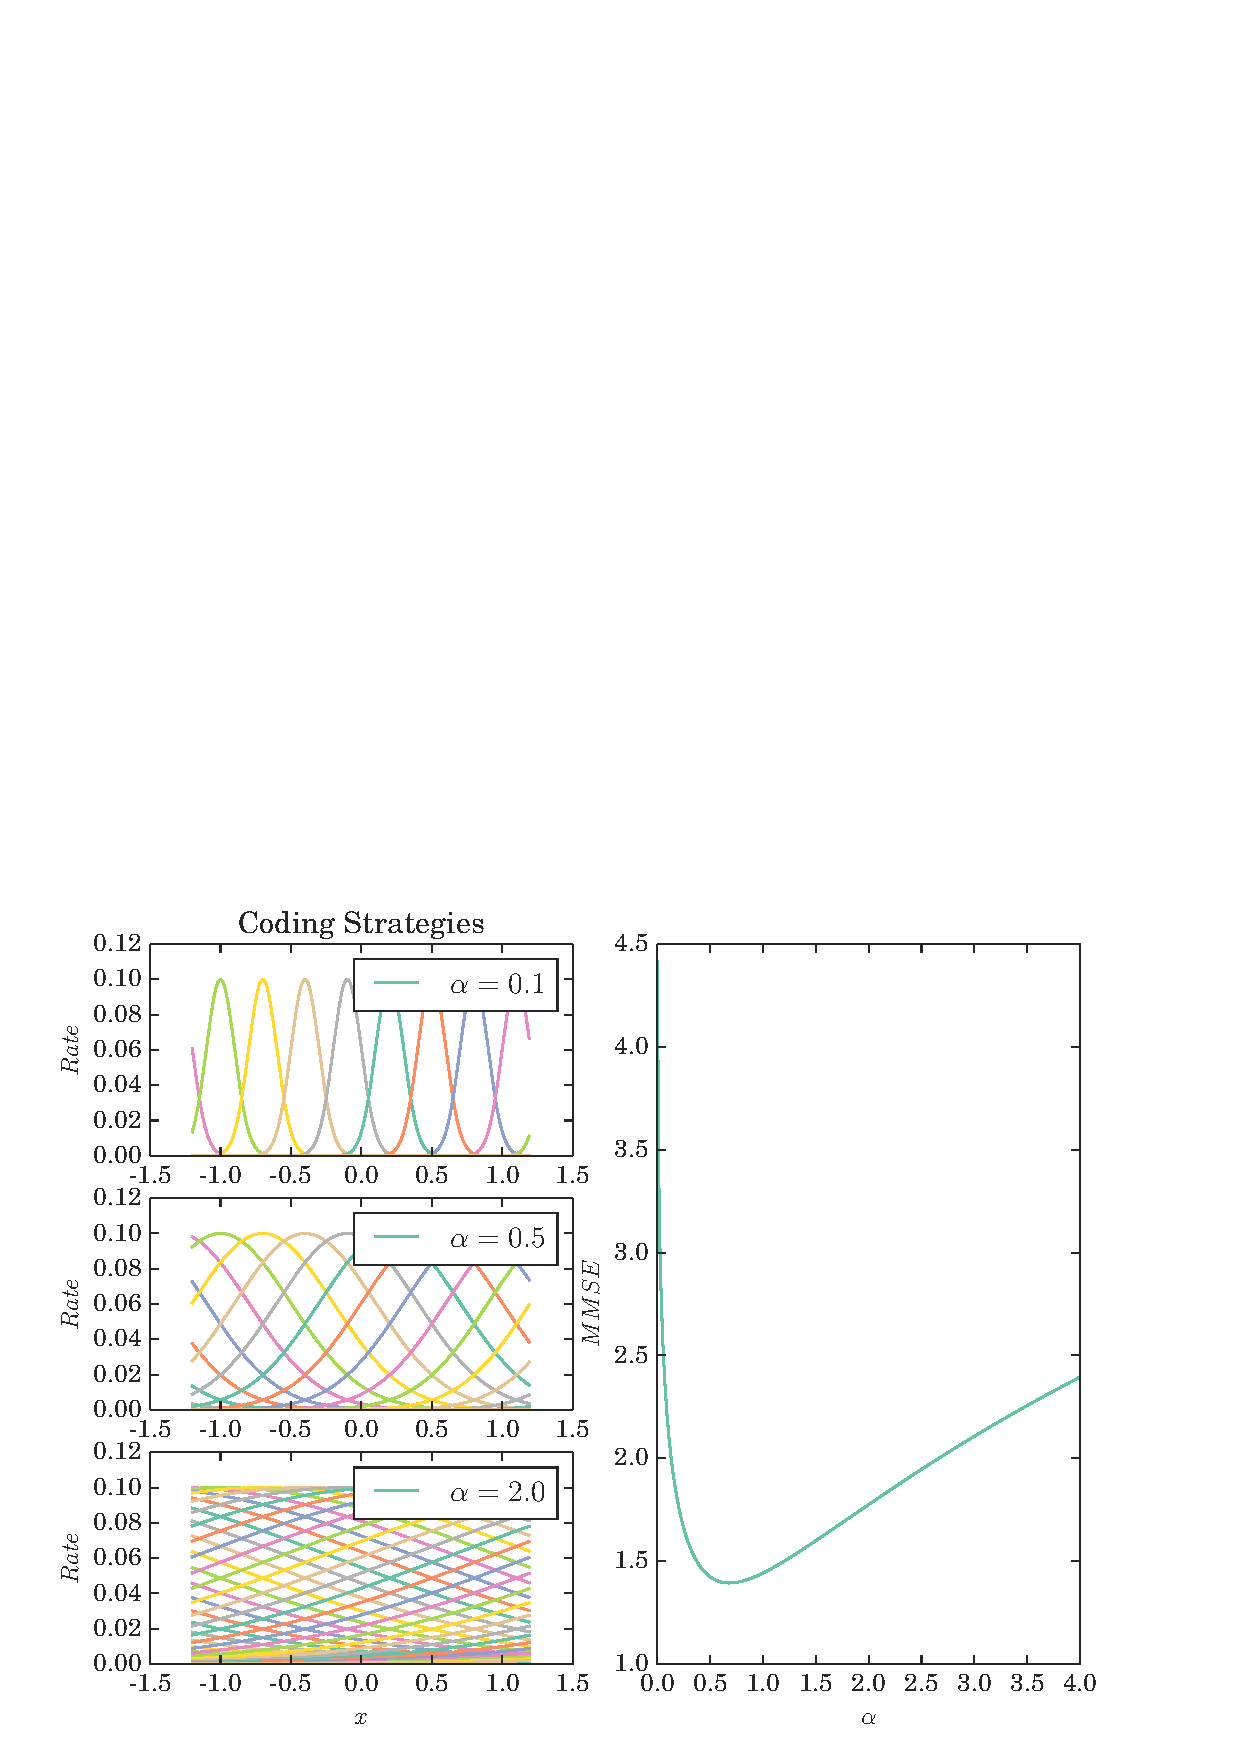
\includegraphics[width=\columnwidth]{figures/figure_5_1.pdf}
\caption[Optimal coding for filtering.]{Optimal coding for filtering Problems: The leftmost column shows the tuning curves of the neurons in the population. Meanwhile, the middle column
shows the general setup of the filtering scheme for each population for the same stochastic process. Note the different situations for narrow and broad tuning curves.
The rightmost plot shows the MMSE as a function of the tuning width $\alpha$.}
\end{figure*}

\subsection{Optimal Codes for Control}

In \fref{chap:control} I have introduced the formalism of stochastic optimal control and shown how to extend it to deal with point process observations. In a similar way
as one can define an optimal encoder for a filtering problem, one can define an optimal encoder for a control problem. Given a control problem with a cost function
\[
C(\boldsymbol{N}_{[0,T]},U_{[0,T]}) =\boldsymbol{E}\left[ \int_0^T c(X(t),U(\boldsymbol{N}_{[0,t]})) dt\mid \boldsymbol{N}\right],
\]
one can define the optimal encoder to be the one with parameters $\varphi^*$ given by
\[
\varphi^* = \argmin_\varphi C(\boldsymbol{N}_{[0,T]},U_{[0,T]};\varphi).
\]
This can lead to different results than the filtering framework as  I will show below.\mycite{Susemihl2014}\par

\subsection{Dense Gauss-Poisson Populations}

In this chapter I will mostly discuss results regarding dense populations of Gauss-Poisson neurons. So, unless otherwise noted, I am discussing a population of Poisson neurons
with tuning functions $\lambda^m(x)$ given by
\begin{equation}
\label{eq:tuning_function}
\lambda^m(x) = \phi \exp\left[-\frac{1}{2} (x-\theta_m)^\top \covar^\dagger (x-\theta_m)\right].
\end{equation}
When the stimulus is one-dimensional, I will denote the covariance of the tuning function by $\alpha$ instead of $\covar$.\par
The dense coding property holds if the overall firing rate of the population $\hat{\lambda} = \sum_i \lambda^i(x)$ is independent of the stimulus $x$. I will refer to a population
of Poisson neurons with Gauss tuning functions such that the dense coding property holds as a dense population of Gauss-Poisson neurons.


\section{Filtering Linear Stochastic Processes through dense Gauss-Poisson Spike Trains}

Consider a linear stochastic process of the type
\[
dX(t) = AX(t) + H^{1/2} dW(t).
\]
Though this may seem as a somewhat restrictive choice, a number of processes can be cast into this format. The simple Ornstein-Uhlenbeck process, which I considered in
previous chapters is one example, but generalisations to higher dimensions are relatively simple and include, for example, the stochastic damped oscillator. The matrices
\[
A= \left(\begin{array}{cc} 0 & 1\\ -\omega^2&-2 \gamma\end{array}\right), \textrm{ and }H= \left(\begin{array}{cc} 0 & 0\\ 0& \eta \end{array}\right),
\]
will lead to a stochastic process with a periodic component, more precisely the stochastic damped oscillator given by the system of SDE's
\[
\dot{X}(t) = V(t), \quad dV(t) = -2 \gamma V(t)dt -\omega^2 X(t) dt + \eta dW(t). 
\]
I have here written a pre factor of $2$ to the damping coefficient, so that the choice $\gamma = \omega$ leads to the critically damped stochastic oscillator.
This is an example of embedding a non-Markov one-dimensional process in a higher-dimensional space to recover the Markov property, as described in \fref{sec:stochastic_proc}.
In \fref{fig:stoch_example} a few examples of linear stochastic systems are shown, with a couple of 
random samples of each per plot. Although the focus here is on stationary stochastic processes,
this is by no means a necessity for the analysis at hand. Even for non-stationary processes such as the Wiener process,\marginnote{The Wiener process $W(t)$, for example, has
a covariance that increases linearly with time.} the posterior density can be stationary, allowing us to evaluate the stationary MMSE.\par

\begin{figure}
\label{fig:stoch_example}
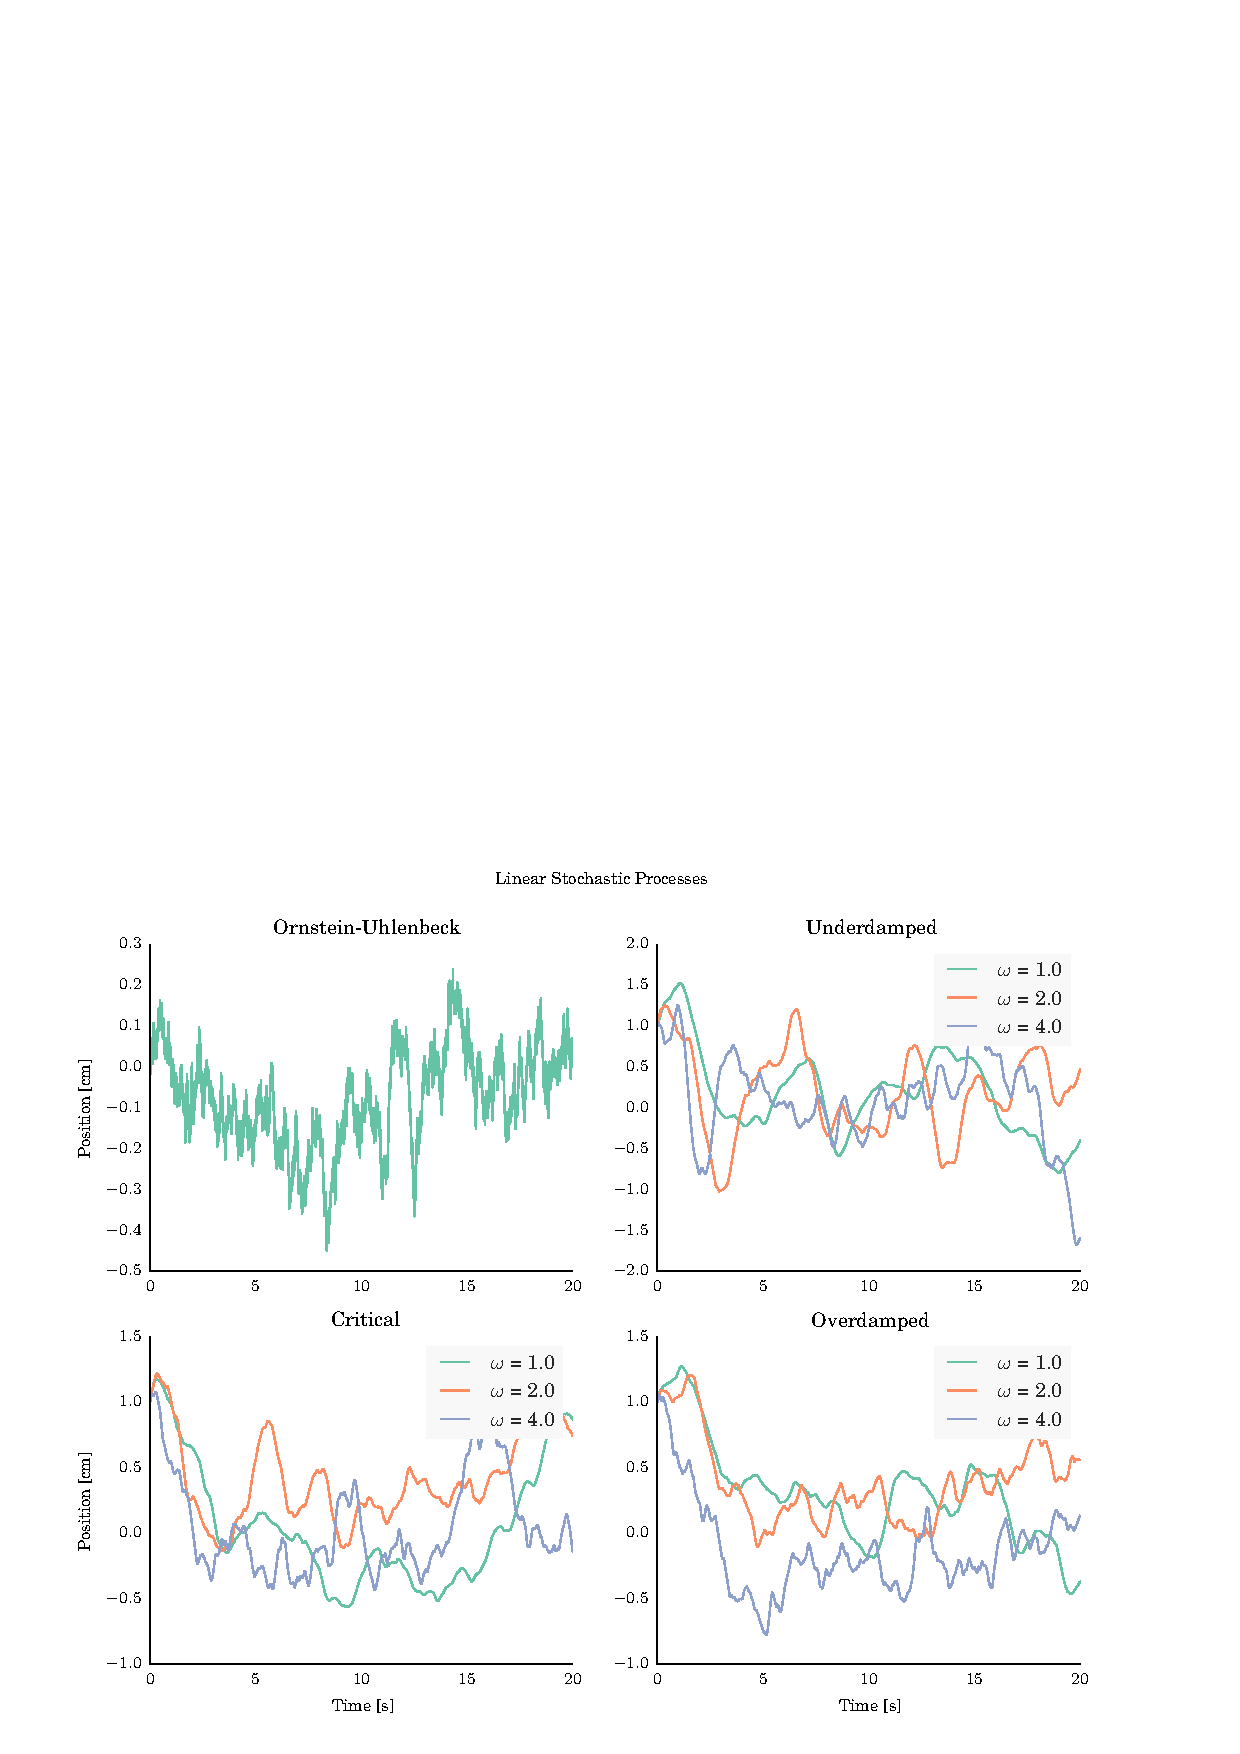
\includegraphics[width=\columnwidth]{figures/figure_5_2.pdf}
\caption[Samples of linear stochastic processes.]{Linear stochastic processes: From the top left, we have the one-dimensional Ornstein-Uhlenbeck process, an underdamped stochastic oscillator,
a critically damped stochastic oscillator (bottom left), and an over damped stochastic oscillator.}
\end{figure}


The MMSE $\epsilon(t)$ can be obtained from the formalism derived in \fref{chap:mse}. Throughout this section I will use both the numerical solution of the
evolution equations for $\epsilon(t)$ as well as the mean-field approximation to it.\par

Let me start with the simplest stationary stochastic process, the Ornstein-Uhlenbeck process
given by
\[
dX(t) = -\gamma X(t) dt + \eta^{1/2} dW(t),
\]
where the exact evolution of the MMSE is given by
\[
\frac{d\epsilon(t)}{dt} = -2\gamma \epsilon(t) + \eta -\hat{\lambda} \boldsymbol{E}\left[\frac{s^2}{\alpha^2+s}\right].
\]
I will not consider the temporal evolution of the MMSE, instead
I will focus on the stationary value of the MMSE, and therefore on the long-term performance of the encoder in the filtering problem, rather than focusing
on the transient, short-time behaviour. I am mostly interested in the dependence of the optimal encoder in the statistical structure of the stimulus, i.e. the correlation
timescales and the noise levels. In a natural environment, these changes should be generally slower than the adaptation processes of the sensory apparatus. This is my main
motivation to focus on the stationary regime.\par
In \fref{fig:mmse_ou} the equilibrium MMSE of a dense Gauss-Poisson population of neurons encoding
an OU process is shown. The dependence on both the maximal firing rate $\phi$ and the tuning width $\alpha$ is shown.

\begin{figure*}
\label{fig:mmse_ou}
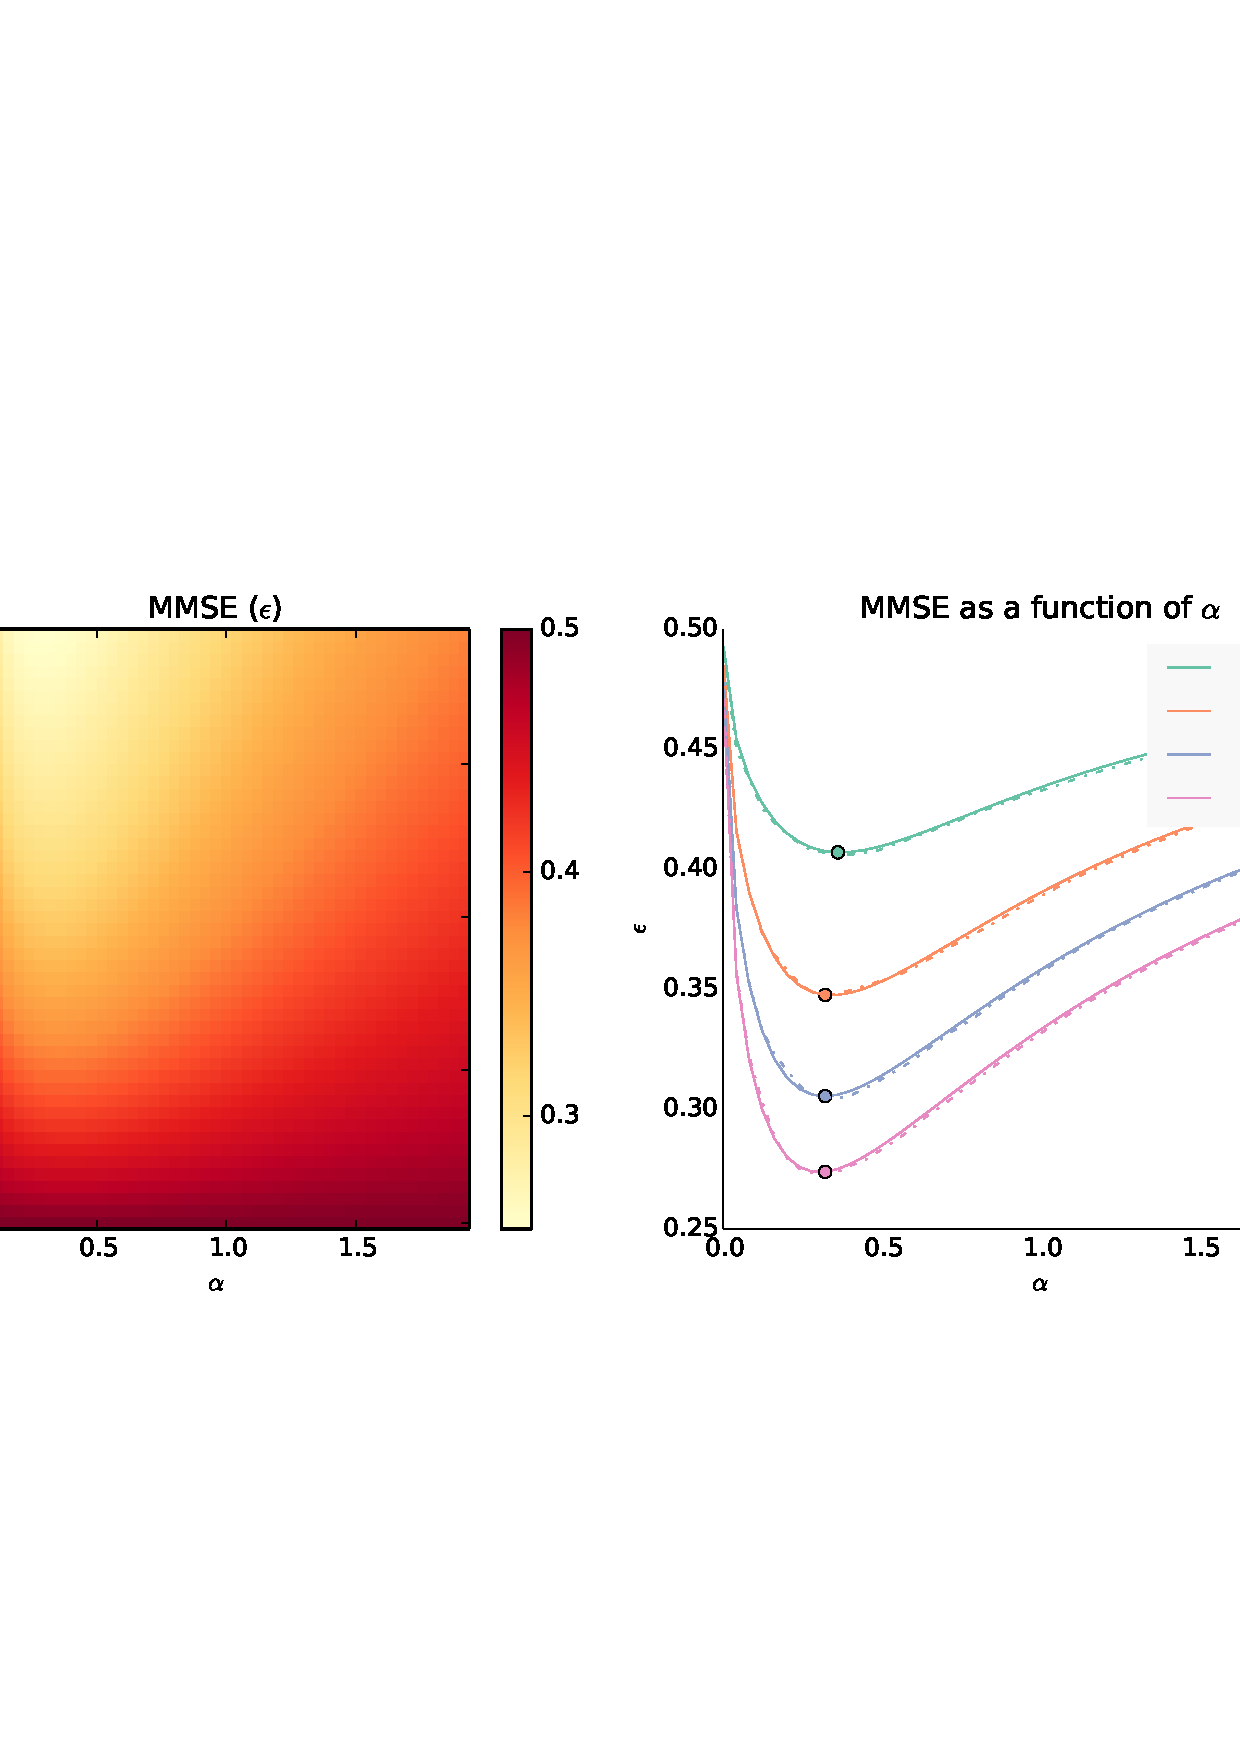
\includegraphics[width=\columnwidth]{figures/figure_5_3.pdf}
\caption[Optimal encoding for the OU process.]{Comparing Encoders for Filtering: The left hand panel shows a heat map of the MMSE as a function of the maximal firing rate $\phi$ and the tuning
width $\alpha$. There is a trade-off between the number of spikes and the precision of the spikes, manifesting itself in a finite tuning width that minimises the
the MMSE. For any $\alpha$ increasing the firing rate $\phi$ simply decreases the MMSE. The right panel shows the dependence in $\alpha$ for a few values
of $\phi$.}
\end{figure*}

More interestingly, one can now ask how the optimal encoder depends on any of the parameters of the problem, such as the parameter $\gamma$, for example,
which defines the time-scale of correlations in the OU process.\footnotemark
In \fref{fig:ecological_ou} I have plotted the optimal encoding width $\alpha^*$ as a function of $\gamma$, $\eta$ and
$\phi$. It is interesting to be able to provide an accurate account of the dependence of the optimal 
encoder on the statistical structure of the environment. The leftmost panel shows the dependence of the optimal tuning width in $\gamma$. Shorter time-scales (larger values of $\gamma$) require a higher frequency of spikes, as the information conveyed by those spikes becomes irrelevant
more quickly.\footnotetext{Remember that the prior kernel of the OU process is given by $k(s,t) = \frac{\eta}{2\gamma} \exp(-\frac{|s-t|}{2\gamma})$.} Thus, holding the maximal firing rate $\phi$ fixed, the only way to increase the frequency of spikes is to have broader tuning functions. Therefore, as $\gamma$
increases, so does $\alpha^*$. Likewise, a higher noise rate $\eta$ leads to the need for more spikes to characterise the system's state, leading to higher values
of $\alpha^*$. Increasing the maximal firing rate $\phi$ of the neurons, on the other hand, leads to smaller optimal tuning widths $\alpha^*$.


\begin{figure}
\label{fig:ecological_ou}
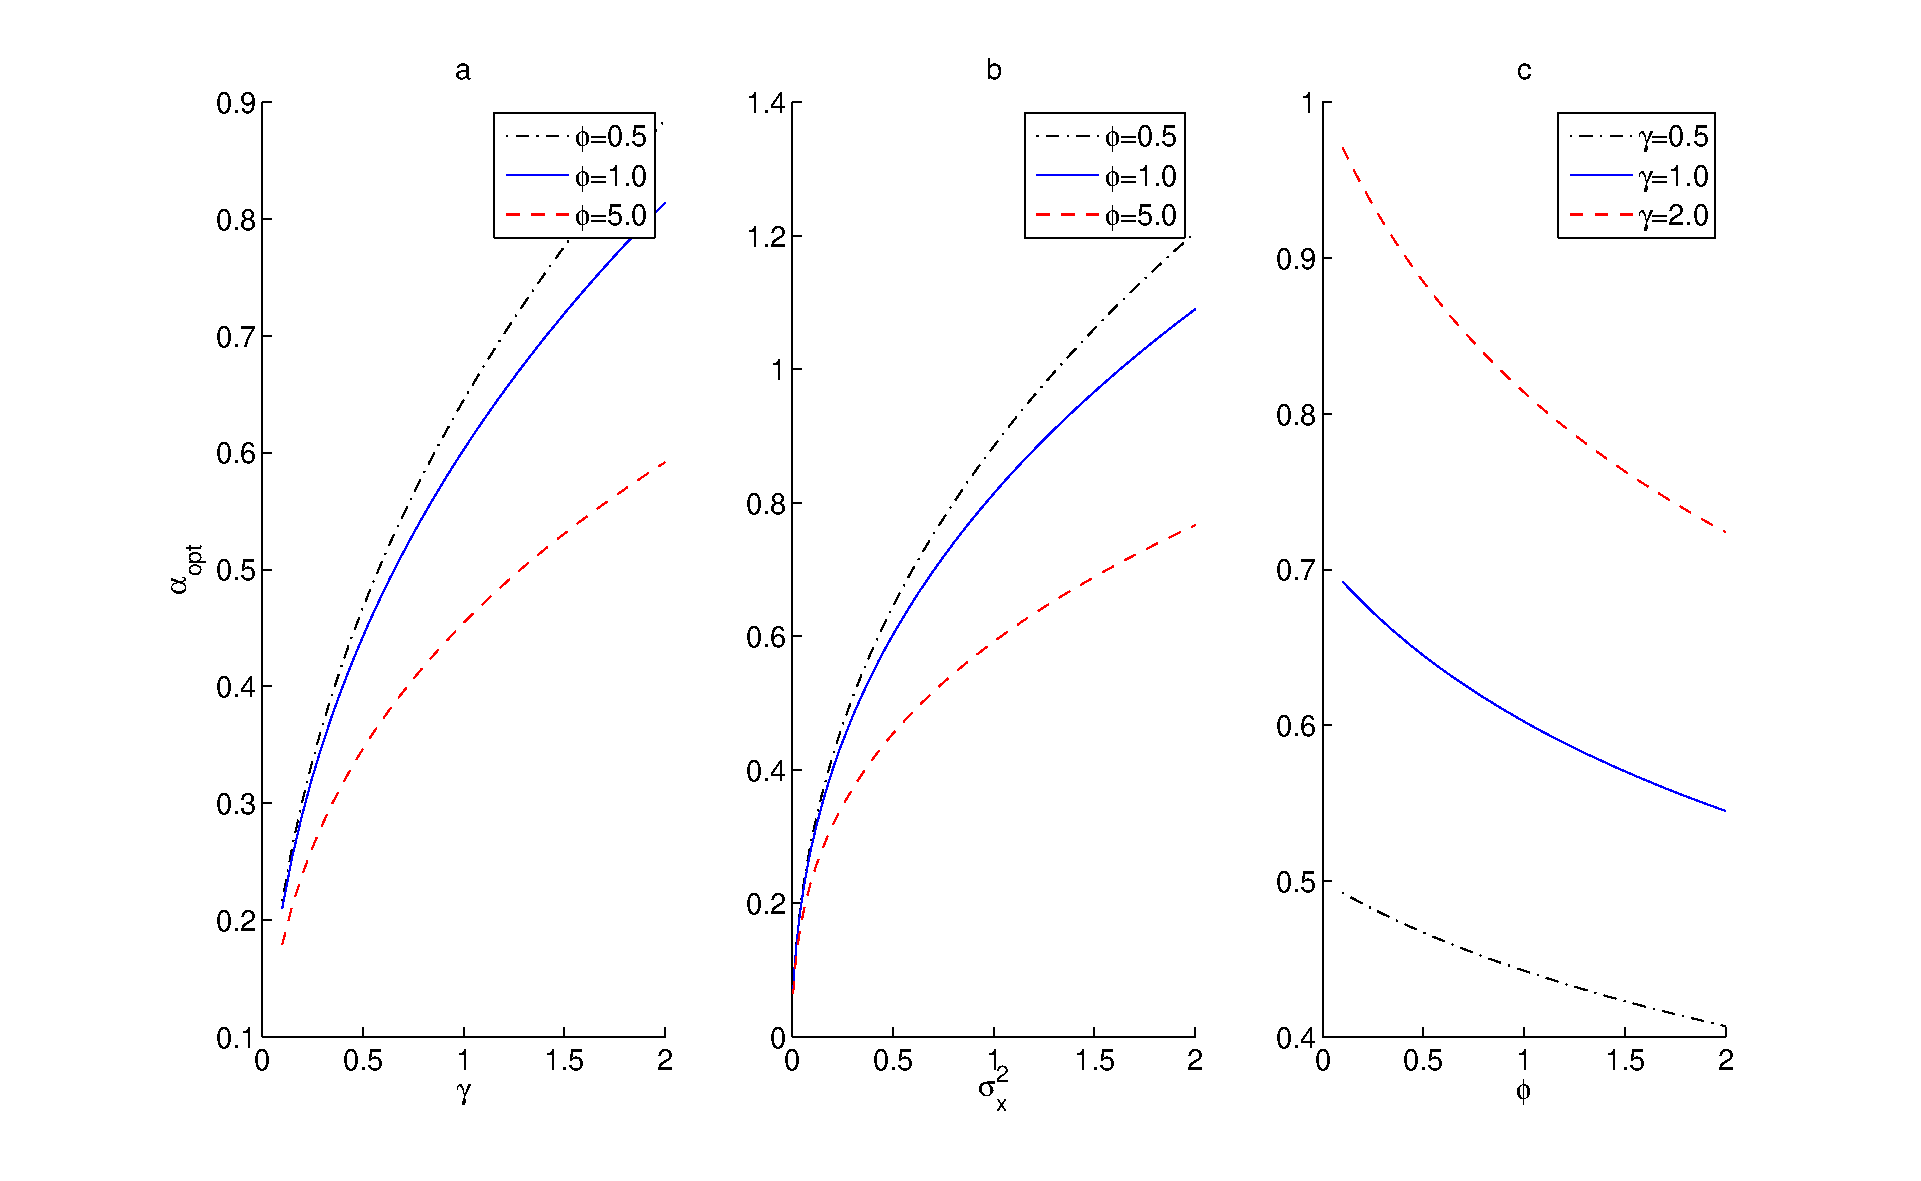
\includegraphics[width=\columnwidth]{figures/figure_5_4.eps}
\caption[Ecological dependence of the optimal encoder.][50pt]{Ecological Dependence of the Optimal tuning width for a dense population of Gauss-Poisson neurons encoding the state of an OU process. Increasing the timescale of the correlations $1/2\gamma$ leads to smaller optimal tuning widths, this can be seen in (a). (b) An increase in the noise rate of the process leads to larger optimal
tuning widths, as an increase in the variance of the process requires more observations to characterise it. (c) The maximal firing rate of each neurons $\phi$ sets the tradeoff
between frequency and precision of the observations. A higher firing rate, tilts the tradeoff towards more precise observations, leading to smaller optimal tuning widths. }
\end{figure}

\subsection{Stochastic Harmonic Oscillator}
A natural extension to consider is the same setup but with the stimulus given by the stochastic harmonic oscillator presented above. Here I will consider a population of neurons whose
firing rate depends only on the position of the oscillator, not on the velocity. This would be equivalent to taking the tuning matrix
\[
\covar = \left(\begin{array}{cc} \alpha^2 & 0\\0&0\end{array}\right),
\]
leading to the same form of the tuning functions as before.
The results are very similar to the OU case, 
regardless of the smoother nature of the process considered. In \fref{fig:mmse_osc} the MMSE for a dense Gauss-Poisson population coding for
a stochastic oscillator is shown. Likewise, \fref{fig:ecological_osc} presents the dependence of the optimal tuning width on the parameters of the encoder and the environment.
There are three parameters determining the dynamics of the environment, the frequency $\omega$, the damping $\gamma$ and the noise rate
$\eta$, and I have presented the dependence of the optimal tuning width on all three. Interestingly, in \fref{fig:ecological_osc} (c), one can note a quite different behaviour for the
stochastic oscillator. The case $\gamma=0.5$ represents an underdamped oscillator, $\gamma=1$ is the critically damped oscillator and $\gamma=5.0$ an over damped oscillator.
First one can note that the dependence of the optimal tuning width on the firing rate $\phi$ is much less pronounced than in the OU process. This is to be expected, as the stochastic
oscillator has a smoother structure, and allows one to predict it from past observations more reliably. It can also be noted that the effect of increasing the firing rate on the optimal
tuning width is strongest in the underdamped regime, which can also be understood by looking at \fref{fig:stoch_example}. When increasing the damping coefficient $\gamma$, the
stochastic variations in the velocity become smaller, and the system's state $X(t)$ has smaller, shorter time-scale variations around $X(t)=0$, while the overall variance of the process
also becomes smaller.

\begin{figure*}
\label{fig:mmse_osc}
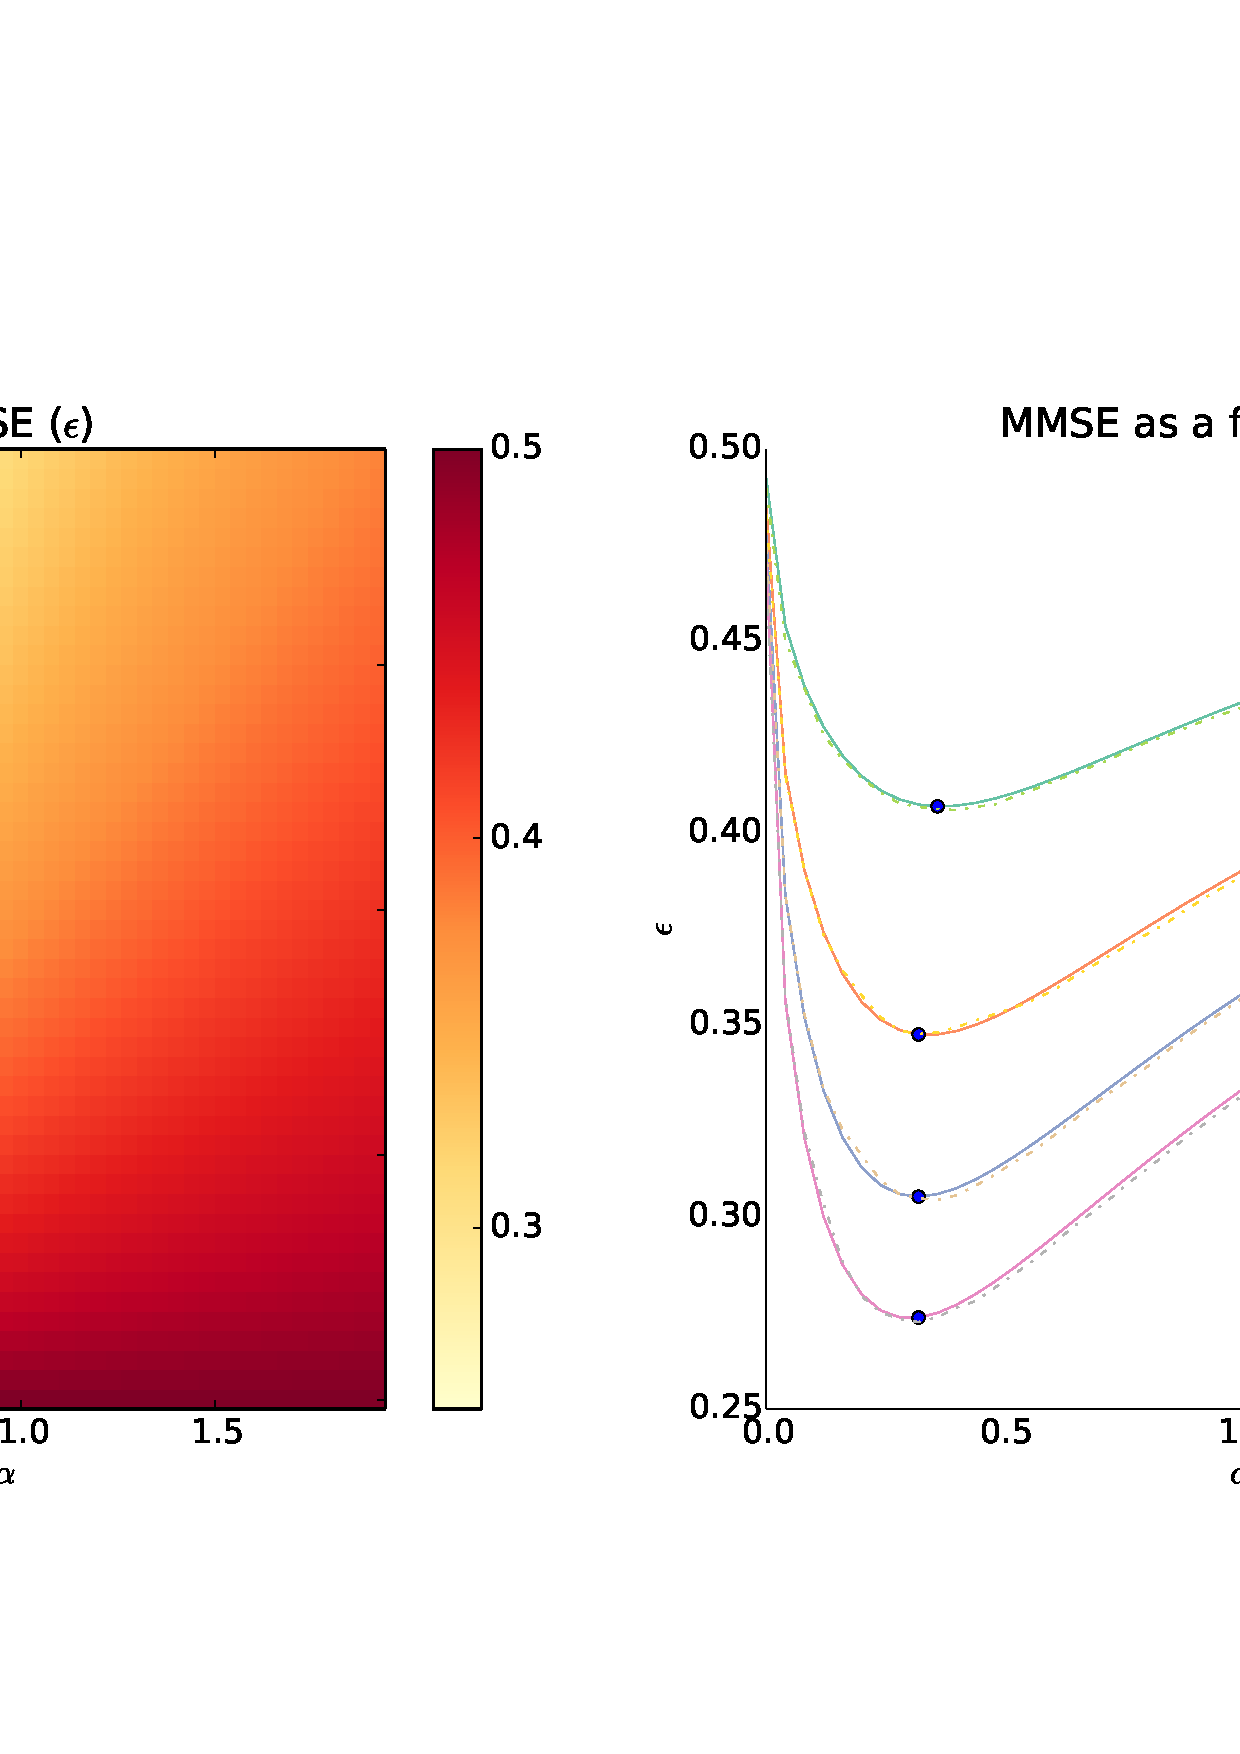
\includegraphics[width=\columnwidth]{figures/figure_5_5.pdf}
\caption[Optimal encoders for the stochastic harmonic oscillator.]{Comparing Encoders for Filtering: The left hand panel shows a heat map of the MMSE as a function of the maximal firing rate $\phi$ and the tuning
width $\alpha$. There is a trade-off between the number of spikes and the precision of the spikes, manifesting itself in a finite tuning width that minimises the
the MMSE. For any $\alpha$ increasing the firing rate $\phi$ simply decreases the MMSE. The right panel shows the dependence in $\alpha$ for a few values
of $\phi$.}
\end{figure*}

\begin{figure}
\label{fig:ecological_osc}
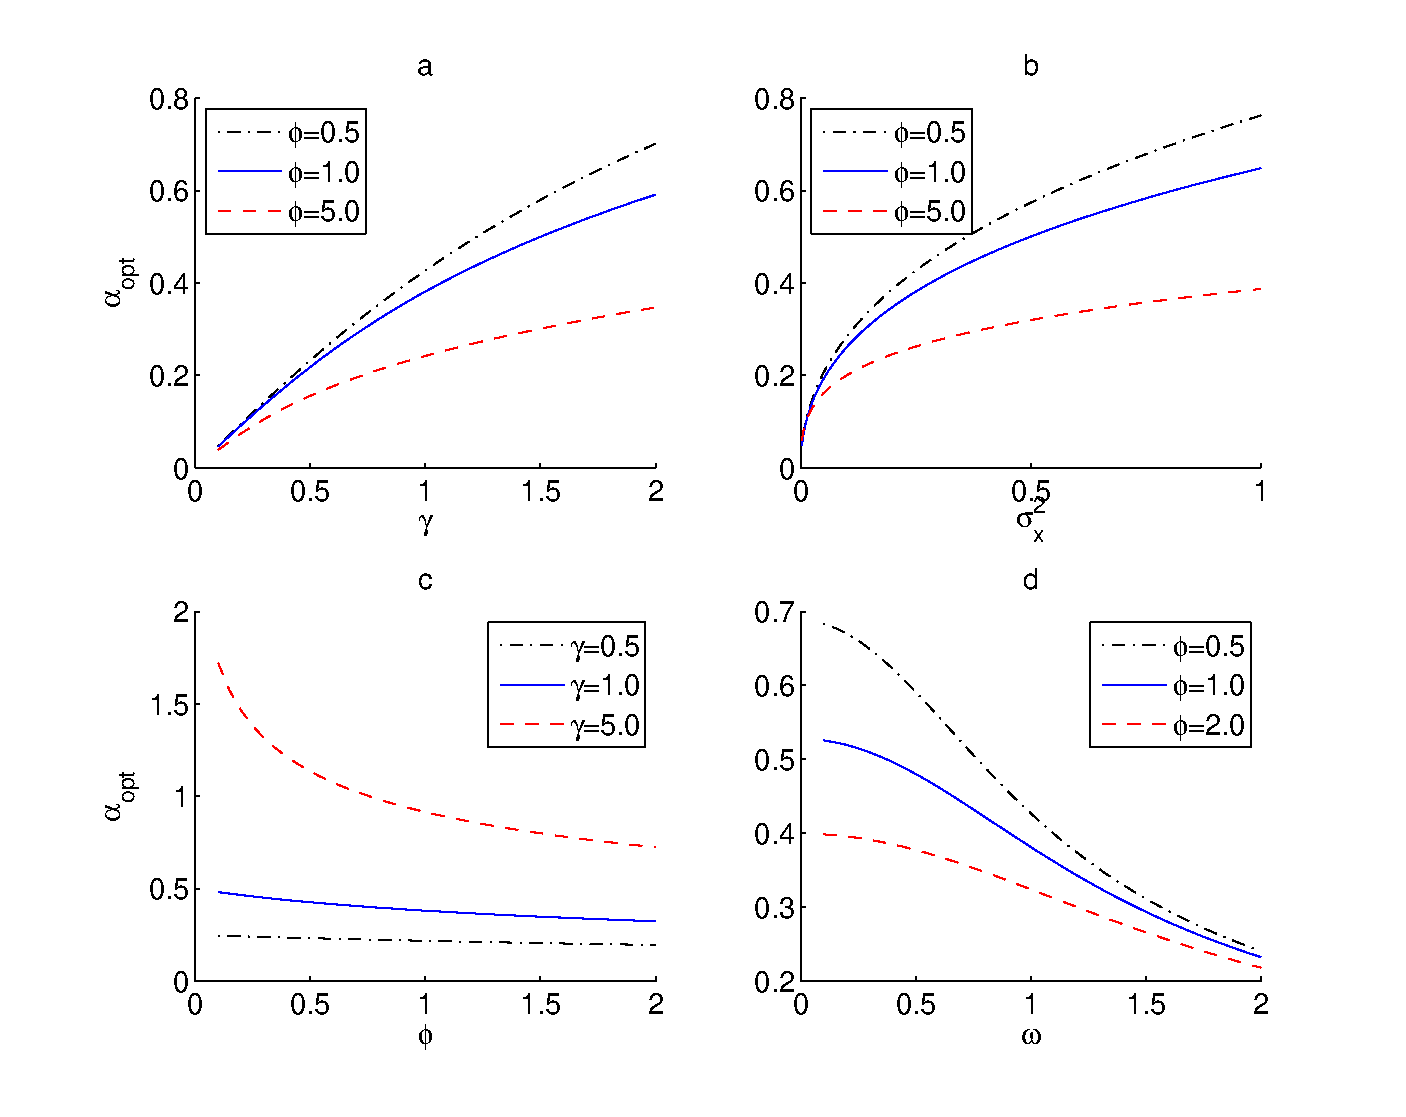
\includegraphics[width=\columnwidth]{figures/figure_5_6.eps}
\caption[Ecological dependence of the optimal encoder for the stochastic oscillator.][50pt]{Ecological Dependence of the Optimal tuning width for a dense population of Gauss-Poisson neurons encoding the position of a stochastic oscillator. The effect of the damping is similar to the effect of the
parameter $\gamma$ in the OU case, as it sets the time-scale of fluctuations in the velocity, which in turn drives the position being estimated. Lower $\gamma$ lead to longer time correlations in the velocity and also in the position, leading to easier reconstruction and a narrower optimal tuning width. The noise intensity $\eta$ also has the same effect as in
the OU process, as a stronger noise leads to wider optimal tuning widths. The maximal firing rate of each neuron $\phi$ has a much less pronounced effect on the optimal tuning width
than in the OU case, specially for the critical and overdamped regime. This is due to the smoother nature of these processes. The  frequency of the process, surprisingly, has the 
inverse effect as the damping, with higher frequencies leading to lower optimal tuning widths. This is due to the damping effect it has on the velocity, leading to a shorter integration
time for the noise in the velocity.}
\end{figure}

\subsection{Smooth Processes}

Through the kernel process formulation developed in \fref{sec:kernels} one can also treat general Gaussian processes, even non-Markov ones such as the RBF process.
By non-Markov processes, I mean processes which can not be rendered Markovian by the inclusion of its derivatives in a higher-dimensional embedding.
The MMSE is given by the average posterior variance of the Gaussian process regression, $\boldsymbol{E}_{\{t_i\}}\left[\Xi(t,t;\{t_i\})\right]$, which can be approximated by the 
mean-field posterior kernel $g(0)$.\footnote{See \fref{sec:kernels} and \fref{app:kernel_integral}.}
In \fref{fig:mmse_rbf} I have evaluated the kernel mean-field approximation for the RBF kernel $k(s,t) = \exp\left(-(s-t)^2/L\right)$, with $L= 0.5$. Note that the general
conclusions drawn in the two previous cases hold here as well, regardless of the more complex temporal structure of the process.\par

In the case of linear stochastic processes, I had found that the temporal mean-field approximation of \fref{eq:eps_mf} was surprisingly good at describing the average
behaviour of the posterior variance. Therefore it is interesting to study how the mean-field approach performs in the RBF case, where the filtering error is derived from
an approximation to the posterior kernel. To that intent, I can evaluate the average posterior variance from \fref{sec:kernels} numerically.
This can be done by generating a large number of Poisson spike trains and evaluating the posterior covariance $\Xi(t;\{t_i\})$ for each and taking an average.
This is also shown in \fref{fig:mmse_rbf} as the dotted lines.
The averaging in this case is much more costly, as for every set of $M$ spike times, one needs to invert an $M\times M$ matrix, which takes of the order of $M^3$ operations.
As can be seen from the figure, the mean-field approximation still agrees very well with the numerical average, leading to undistinguishable optimal tuning widths.

\begin{figure*}
\label{fig:mmse_rbf}
\includegraphics[width=\columnwidth]{figures/figure_5_7.pdf}
\caption[Optimal encoders for the RBF process.]{MMSE for a dense population of Gauss-Poisson neurons encoding a RBF process. The MMSE follows the same trends as for the OU process and the stochastic
harmonic oscillator. The dotted lines show the numerically averaged MMSE, obtained directly from the Gaussian process regression.}
\end{figure*}

\section{Moving Away From Gaussian Distributions}

In \fref{chap:filtering} I have presented filtering tools for general stochastic processes and observation processes, namely the ADF and particle filter techniques.
So far, in the analysis of optimal codes I have restricted myself to the dense coding limit, which significantly simplifies the analysis, rendering the Gaussian ADF approach
exact. What happens when the posterior is not Gaussian, though? I will consider a couple of interesting cases shortly. There are two ways one can leave the dense
coding limit. The first one is to have a population which does not densely cover the stimulus space. The simplest case would be a single neuron with a Gaussian tuning function,\footnotemark for example,
which could clearly not cover the stimulus space. The second possibility refers to the nature of the neurons. If their spiking is time-dependent or adaptive,\footnotetext{See \fref{fig:neuron_example}.} the homogeneity of the firing
rate will break and we will have a stimulus-dependent population firing rate as well. Of course the posterior can also be non-Gaussian due to the prior. That would mean the
process being observed is non-Gaussian. I will consider the simple case of a stochastic process in a double-well potential, as an example of non-Gaussian processes.
\par

Once again my main interest is in the optimality of said codes. It is straightforward to estimate the MMSE of the mentioned cases from simulations directly. 
Though much less practical than the dense coding case, where one could refrain from simulating the stimulus trajectories and spike trains, the principles remain the
same. It is not true, however, that the average posterior covariance gives the MSE of the estimator in this case. Remember that I have used that the estimator is the
posterior average to show that, and this does not hold generally for either the ADF or the particle filter estimator. For the particle filter, it can be shown that
in the limit of many particles the empirical distribution converges to the posterior distribution, yielding the posterior mean estimator in the limit of infinite particles.\mycite{crisan2002} 
The ADF estimator, however, has no simple relation to the posterior mean estimator, and further has no guarantee of converging to the true posterior. So in both cases we are forced 
to work directly with the average estimation error to obtain a measure of the MSE.\par

This section is meant to illustrate the application of the framework of MSE-optimal codes outside of the assumptions made in the previous section. Though optimising a code for
the MSE is not as straightforward for more complex, higher-dimensional problems, this shows that it is in principle possible, and the hurdles are mostly of implementation, rather
than conceptual.


\subsection{Sparse Populations}

The simplest form of breaking the dense coding assumption is, well, not having dense populations. The most extreme case would be if there were only one or
a few neurons coding for the stimulus. In that case, the population firing rate could be very strongly dependent on the state of the system. I will consider a simple
case here to illustrate the applicability of the MSE method. I will consider the case of a population of two neurons, equidistant from the mode of the stimulus distribution,
and investigate the dependence of the MSE on the separation between the two and the width of the tuning functions.\par

I will use three filtering schemes for this problem and compare them. First, I consider
the filtering equations given by \fref{eq:filtering_sdes}. In the dense coding case, these equations are exact, but one can use them as an approximate filtering method
regardless of the population being dense. This amounts to ignoring the probability of a spike not being fired, and looking only at the probability of a spike being fired when a spike is
actually observed. I will refer to this filtering scheme as the Dense ADF approach. A second possibility is to apply the ADF approach with a Gaussian distribution, now taking the rate 
terms in \fref{eq:adf_gauss_filter} into account and updating the mean and covariance through \fref{eq:gaussian_updates} upon the observation of a spike. I will refer to this option as 
the Full ADF approach. A third possibility is to use a particle filter with a large number of particle (I have taken $M=1000$ here) to estimate the posterior probability given the spikes.
This again, takes into  account the probability of a spike not having been fired in every time instant by every neuron.\par

%These approaches are compared in \fref{fig:dense_to_sparse} for a population of neurons separated by $\Delta\theta$ responding to a stimulus given by an OU process.
%As expected, when $\Delta\theta$ is very near zero, the schemes are virtually indistinguishable, however, as $\Delta\theta$ grows, the dense ADF approach gives a substantially
%larger MSE than the two other approaches, showing that this approach is only appropriate for small values of $\Delta\theta/\alpha$. Note that the MSE grows for all three approaches,
%since increasing $\Delta\theta$ lowers the overall firing rate, leading to fewer spikes, and therefore poorer MSE performance. The lowest MSE (therefore the one nearest the MMSE)
%is given by the particle filter, therefore I will choose to use the particle filter when no exact solution is obtainable. The Full ADF approach does not fare much worse, though, and it
%is still an interesting filtering method in practical applications as it does not require the simulation of multiple particles.\par
%
%\begin{figure}
%\includegraphics[width=\columnwidth]{figures/figure_5_15.pdf}
%\caption[Violating the dense coding assumption]{The violation of the dense coding assumption. As $\Delta\theta$ increases, the dense ADF approach performs poorly in comparison to the other two, showing the violation
%of the dense coding assumption. Of all three methods, the Particle filter shows the lowest MSE, therefore lending itself to an estimation of the MMSE.}
%\label{fig:two_neurons}
%\end{figure}
%

Assuming both neurons have Gaussian tuning functions with the same tuning width, one could ask
what is the best tuning width and spacing between the two neurons to optimise the MSE. In \fref{fig:two_neurons} I have plotted the MSE as a function of $\Delta\theta$ and
$\alpha$, showing a clear optimum. There are some artefacts due to the interplay of $\alpha$ and $\Delta\theta$, but all three approaches show a clear minimum. Surprisingly, even
in this case, the dense ADF approach yields nearly the same MSE as the particle filter or the full ADF approach, showing a relative absolute deviation from the full ADF approach of
less than 1\% and of approximately 1.5\% from the particle filter approach. This might be due to the Gaussian nature of the stimulus, but
it is an interesting point for further investigation.\par

\begin{figure}
\includegraphics[width=\columnwidth]{figures/figure_5_14.pdf}
\caption[Optimal coding with two Gaussian neurons.]{Two neurons with Gaussian tuning functions coding for a simple OU process. The left panel shows two sample tuning functions, explaining the parameters $\Delta\theta$ and
$\alpha$. The left panel shows the MSE according to the different approaches. The top shows the ADF approach assuming a dense population (i.e. ignoring the firing rates in the 
absence of spikes). The middle plot shows the MSE obtained with a full Gaussian ADF approach. The bottom plot shows the MSE of a particle filter. Though the three approaches
give different results, the general dependence of the encoder on the parameters is clear for all three approaches. There is an optimal value of $\Delta\theta$ and $\alpha$
which minimises the MSE in all three approaches}
\label{fig:two_neurons}

\end{figure}

\subsection{Adaptive Neurons}

A different situation which could lead to non-uniform firing rates is adaptation in the firing rate of the neurons, even in a dense population of neurons. The spike-frequency adaptation
process described in \fref{sec:ADF} is a simple model where the essence of neural adaptation is already present. I will consider the impact of adaptation
on the MMSE of a simple linear stochastic process as we have considered above.\par

\begin{figure}
\label{fig:adaptive_mse}
\includegraphics[width=\columnwidth]{figures/figure_5_8.pdf}
\caption[MSE of a population of adaptive neurons.]{The MSE of a reconstruction task from the observation of adaptive spike trains. The product $\tau\delta$ quantifies the intensity of the adaptation. As in the previous cases,
one can note the existence of a finite optimal tuning width.}
\end{figure}

A number of interesting questions arise with respect to adaptation in neurons. The adaptation implemented by the spike rate modulation $\kappa(t)$ is similar to the
spike-frequency adaptation often described in neuroscience.\mycite{benda2003} As can be seen in \fref{fig:adaptive_mse}, at first glance it
would seem that adaptation does not help the population code. This is somewhat misleading, though, as the stronger the adaptation time-scale $\tau$, the lower
the firing rate of the population. It would make sense, then to compare adaptive and non-adaptive populations with the same firing rate, to account for the effect of the
adaptation. This is shown in \fref{fig:adaptive_rate_distortion}. Here the mean-squared error of the filter is plotted as a function of the firing rate of the population, and it
is immediately obvious that the adaptive populations achieve a better performance with a much lower firing rate.\par

\begin{figure}
\label{fig:adaptive_rate_distortion}
\includegraphics[width=\columnwidth]{figures/figure_5_9.eps}
\caption[MSE for adaptive neurons as a function of population firing rate.]{MMSE of adaptive population as a function of the population firing rate. Though the adaptation leads to a worse reconstruction error when keeping all other parameters fixed,
here one can see that it allows for a more precise reconstruction with the same amount of spikes. There is a saturation in the improvement however, as the adaptation puts a limit
on the number of spikes the population can fire.}
\end{figure}

\subsection{Nonlinear Stochastic Processes}

A different source of non-Gaussian distributions can be found directly in the stochastic process one is modelling as stimuli. A simple model that leads to non-Gaussian
distribution is a stochastic process in a double well potentialo, given by $V(x) = \nu(x+x_0)^2(x-x_0)^2$. This potential will have two
stable points at $x=\pm x_0$. One can then define a stochastic 
system moving in this potential as
\[
dX(t)  = -\frac{dV}{dx}dt + \eta^{1/2} dW(t).
\]
This leads to
\[
dX(t) = 4\nu X(t)\left(x_0 - X(t)^2\right) dt + \eta^{1/2} dW(t).
\]
\Fref{fig:bistable_samples} shows some sample paths from this process.

\begin{marginfigure}
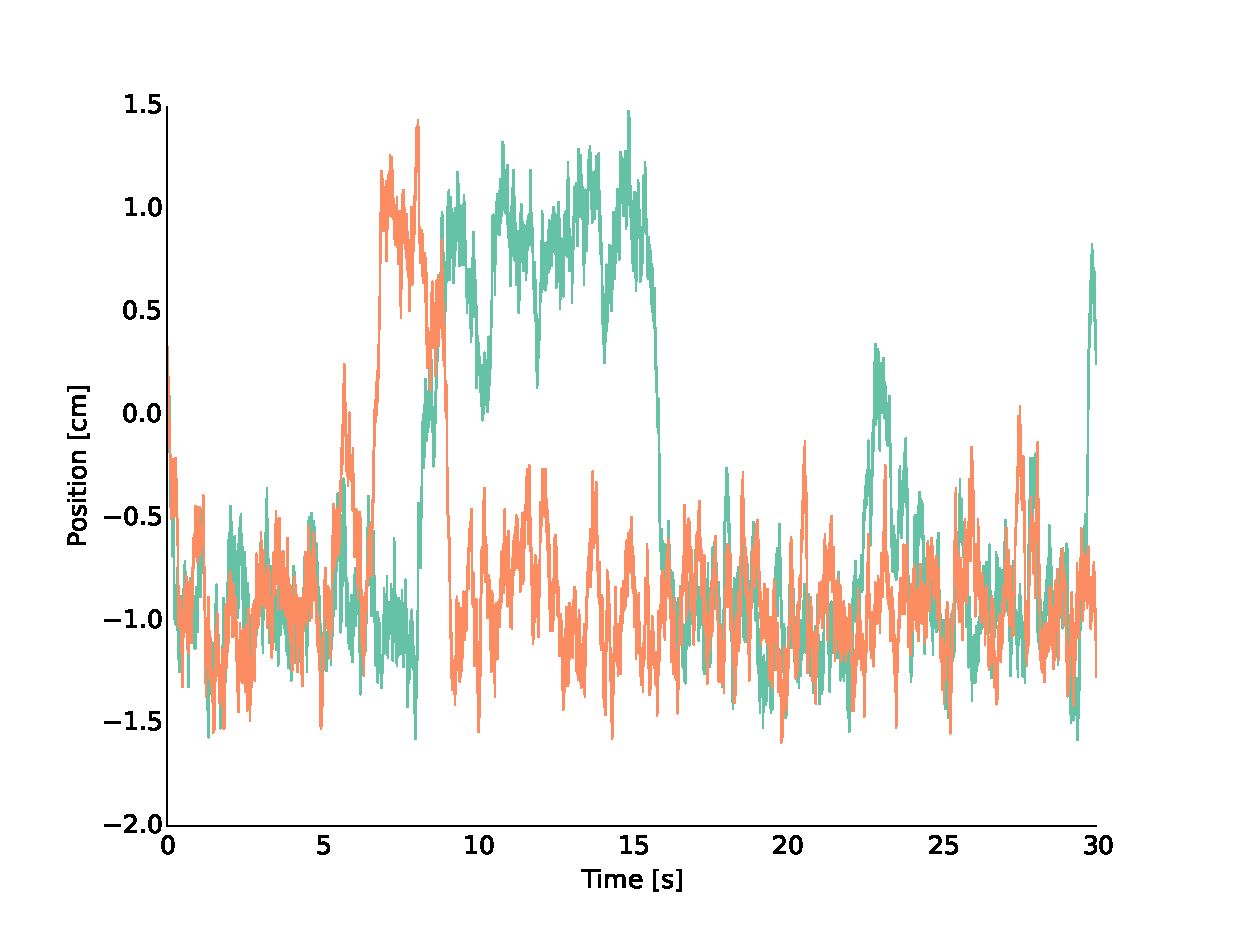
\includegraphics[width=\columnwidth]{figures/figure_5_10.eps}
\caption[Bistable Processes.]{Samples of the Bistable process mentioned in the text.}
\label{fig:bistable_samples}
\end{marginfigure}

Following the framework of \fref{chap:filtering}, it is simple to devise a particle filtering algorithm for this system. Assuming the observations are still from a dense code, one can simply 
take the particles $Z^i(t)$ evolving by the same SDE as the system. So after discretising one will have
\[
\Delta Z^i(t) = 4 \nu Z^i(t) \left(x_0 - Z^i(t)^2 \right) \Delta t+ \sqrt{\Delta t \eta} \,V^i(t) ,
\]
where each of the $V^i(t)$ is a standard normal random variable independent of all other $V^j(t)$. The weights $w^i(t)$ associated with each particle will then be 
updated as 
\[
w^i(t) = w^i(t-\Delta t) \lambda^j\left(Z^i(t)\right),
\]
in case neuron $j$ spikes and simply left unchanged in the absence of spikes. Here $\lambda^j(z)$ are the usual Gaussian tuning functions given by \fref{eq:tuning_function}.\par
Alternatively one can develop an ADF algorithm for the proposed system. Using the relationships derived in \fref{chap:mse} it is easy to obtain the equations for $\mu(t)$ and $\Sigma(t)$,
\begin{subequations}
\begin{equation}
\frac{d\mu(t)}{dt} = 4\nu \mu(t) \left(x_0 -\mu(t)^2-3\Sigma(t)\right) ,
\end{equation}
and
\begin{equation}
\frac{d\Sigma(t)}{dt} = 8\nu \Sigma(t)-24\mu(t)^2\Sigma(t)-24\Sigma(t)^2 + \eta.
\end{equation}
\end{subequations}
\par
In \fref{fig:bistable_filt} I show both approaches applied to the bistable problem. We can then leverage the particle filtering approach, which shows better results
for this filtering problem and look at the optimal tuning width for an estimation task. The MMSE for the bistable process is shown in 
\fref{fig:bistable_optimal}. The general conclusions arrived at previously hold in this setting as well and
the MSE is minimal for a finite tuning width, underlining the trade-off between precision and frequency discussed above.

\begin{figure*}
\label{fig:bistable_filt}
\includegraphics[width=\columnwidth]{figures/figure_5_11.pdf}
\caption[Filtering bistable processes with Point process observations.]{ADF (left) and particle (right) filters applied to the dense Gauss-Poisson coding of a bistable process. Note that the ADF filter consistently underestimates the variance
of the posterior distribution. Leading it to lose track of the system's state at some points.}
\end{figure*}

\begin{figure}
\label{fig:bistable_optimal}
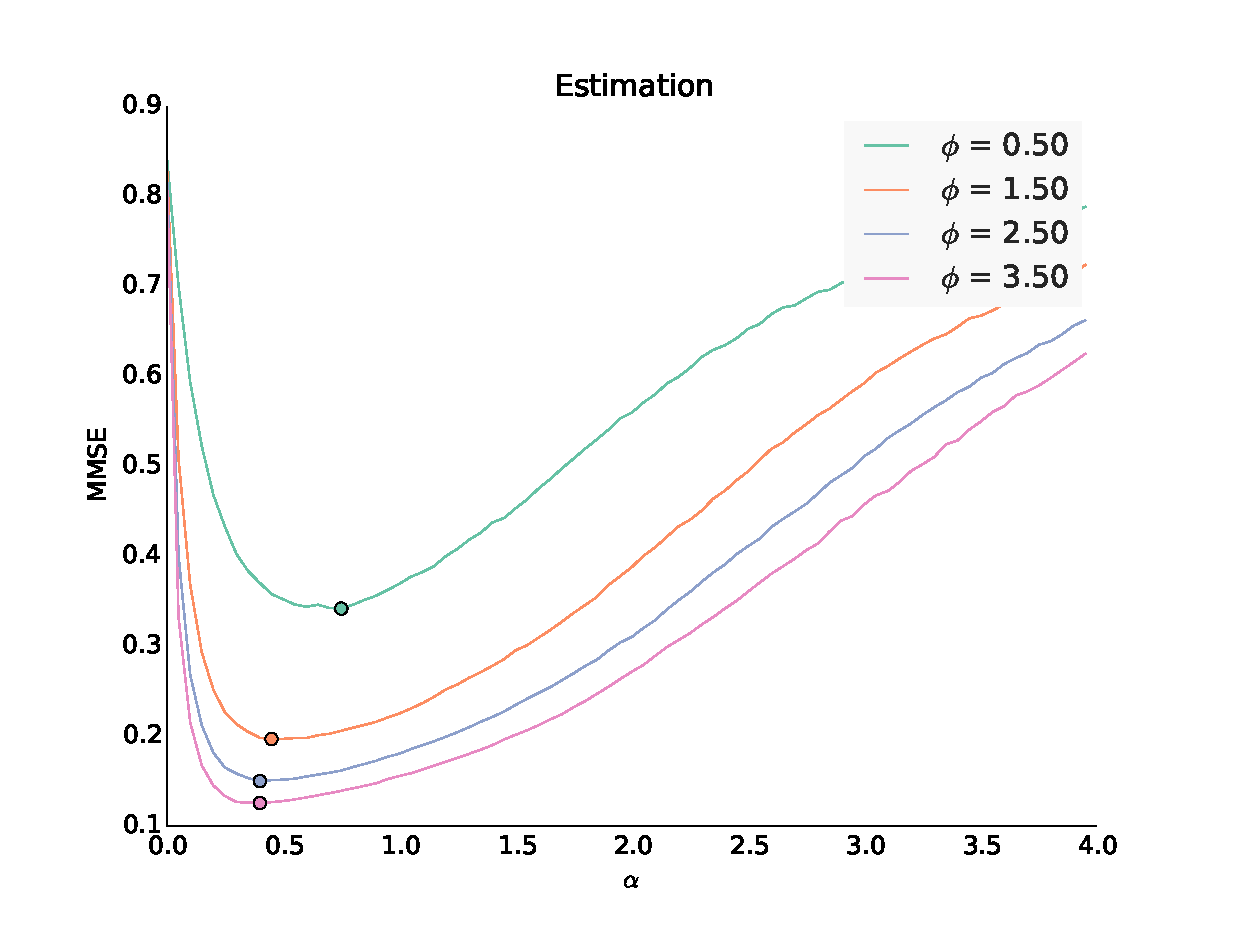
\includegraphics[width=\columnwidth]{figures/figure_5_12_a.eps}
\caption[MSE for the filtering of bistable processes.]{Dependence of the MSE on the tuning width $\alpha$. The width follows the same trend as for the previously considered processes.
The tuning width decreases with increasing firing rates. However, here one can see, that the minimum is less sharp, due to the bistable nature of the process. If a spike allows one
to discern between the two stable states, it already contributes a lot to the estimation of the state $X(t)$.}
\end{figure}

\section{Optimal Codes for Control}

\label{sec:optimal_code_control}

I have extensively argued for the usefulness of accurate estimation of a system's state when interacting with it. Though this is by no mean false, real world
systems are often very high-dimensional, or at least represented in a very high-dimensional code, leading to trade-offs when deciding where to allocate sensory
resources. One simple example is the density of photoreceptors in the retina. If we assume the retina evolved to allow for optimal estimation of the visual scene
facing an animal, we would expect it to cover the entire visual field evenly. That is of course not the case, and there are a number of anomalies in the distribution
of receptive fields which can be attributed to the importance of different visual queues for decision making and risk assessing. A simple example of which is the distribution of photoreceptors in the retina, with the concentration of cones varying up to two orders of magnitude between the periphery and the fovea.\mycite{curcio1987}
\par

What could be the reasons for an optimal code for an estimation problem to be sub-optimal for a control problem? I will present examples that show two possible
reasons for different optimal coding strategies in estimation and control. First, one should note that control problems are often defined over a finite time horizon. One
set of classical experiments involves reaching for a target under time constraints.\mycite{Battaglia2007} If one takes the maximal firing
rate of the neurons ($\phi$) to be constant while varying the width of the tuning functions, this will lead the number of observed spikes to be inversely proportional to
the precision of those spikes, forcing a trade-off between the number of observations and their quality. This trade-off can be tilted to either side in
the case of control depending on the information available at the start of the problem. If one is given complete information on the system state at the initial time $0$,
the encoder needs fewer spikes to reliably estimate the system's state throughout the duration of the control experiment,
and the optimal encoder will be tilted towards a lower number of spikes with higher precision.
Conversely, if at the beginning of the experiment one has very little information about the system's state, the encoder will be
forced towards lower precision spikes with higher frequency.\par

Secondly, one should note that the optimal encoder for estimation does not take into account the differential weighting of different dimensions of the system's state.
When considering a multidimensional estimation problem, the optimal encoder will generally allocate all its resources equally between the dimensions of the system's
state. In the framework presented below one can think of the dimensions as the singular vectors of the tuning matrix $\covar$ and the resources allocated to it as the
singular values. In this sense, I will consider a set of coding strategies defined by matrices $\covar$ of constant determinant.
This constrains the overall firing rate of the
population of neurons to be constant, and one can then consider how the population should best allocate its observations between these dimensions. Clearly, in an
anisotropic control problem, which places a higher importance in controlling one dimension, the optimal encoder for the control problem will be expected to allocate
more resources to that dimension. This is indeed shown to be the case for the Poisson codes considered, as well as for a simple LQG problem with Gaussian observations in 
continuous time when we constrain the noise covariance to have the same structure.\par

\subsection{The Trade-off Between Precision and Frequency of Observations}
\label{sec:information}

In this section I consider populations of neurons with tuning functions as given by \fref{eq:dense_poiss_gauss_tf} having tuning centers $\theta_m$ distributed along a 
one-dimensional line.
In the case of a stimulus modelled by the Ornstein-Uhlenbeck process these will be simply one-dimensional values $\theta_m$ whereas in the case of the stochastic oscillator, I will
consider tuning centres of the form $\theta_m = (\eta_m,0)^\top$, filling only the first dimension of the stimulus space. This means that in the case of the stochastic oscillator, the 
observer does not have direct access to the velocity of the system, only of its position. Note that  in both cases the (dense) population
firing
rate $\hat{\lambda} = \sum_m \lambda_m (x)$ will be given by $\hat{\lambda} = \sqrt{2\pi} \alpha \phi / |\Delta \theta|$, where $\Delta \theta$ is the separation between neighbouring tuning centres $\theta_m$.\par

The OU process controlled by a process $U(t)$ is given by the SDE
\[
dX(t) = (b U(t)-\gamma X(t)) dt + D^{1/2}dW(t),
\]
and the control problem is defined by a cost function
\[
C(X,U) = \int_0^T \left(X(t)^\top Q X(t) + U(t)^\top R U(t)\right)dt.
\]
\Fref{eq:poiss_cost} can then be evaluated by simulating the dynamics of
$\Sigma(t)$. This is exactly the problem solved in \fref{chap:mse} and it has extensively been discussed therein.\footnote{See also \mycitep{Susemihl2013}.}
Following those results one can also approximate the average of the posterior variance by a mean-field formalism which works surprisingly well. The evolution of the 
average posterior variance is given by the average
of \fref{eq:filtering_sde_sigma}, which involves nonlinear averages over the covariances. The mean-field evolution of 
$\boldsymbol{E}\left[\Sigma(t)\middle| \Sigma_0\right]$ is given by
\[
\frac{d\boldsymbol{E}\left[\Sigma(t)\right]}{dt} = A \boldsymbol{E}\left[\Sigma(t)\right] + \boldsymbol{E}\left[\Sigma(t)\right]^\top A^\top + D - \hat{\lambda}  \boldsymbol{E}\left[\Sigma(t)\right]\covar^\dagger  \boldsymbol{E}\left[\Sigma(t)\right] \left(I+\covar^\dagger  \boldsymbol{E}\left[\Sigma(t)\right]\right)^{-1}.
\]
To assess the quality of this approximation I have also computed the averages of $\Sigma(t)$ numerically with a large number of sample paths to compare to the
mean-field approximation. In \mycitep{Susemihl2011a} and \mycitep{Susemihl2013} I had reported a very good agreement in the mean-field and numerically calculated 
values of $ \boldsymbol{E}\left[\Sigma(t)\right]$. $f(\Sigma,t)$ however is an integral over time of this average, so one can expect that the deviation between the mean-field approximation and the 
numerical average will be larger. As can be seen in \fref{fig:comparison_uni}, the mean-field approximation is not as precise as in the case
of the simple average, but the dependence of the average on $\alpha$, however, remains very well explained by the mean-field approach.\par
Alternatively, one can look at a system with more complex dynamics, and I will take as an example the stochastic damped harmonic oscillator given by the system of equations
\begin{equation}
\label{eq:stoch_osc}
\dot{X}(t) = V(t),\quad dV(t)=\left(b U(t)-\gamma V(t)  - \omega^2 X(t) \right)dt + \eta^{1/2} dW(t).
\end{equation}
Furthermore, I assume that
the tuning functions only depend on the position of the oscillator, therefore not giving any information about the velocity. The controller in turn seeks to keep the
oscillator close to the origin while steering only the velocity. This can be achieved by the choice of matrices
\[
A = \left(\begin{array}{cc}0& 1\\ -\omega^2 & -\gamma\end{array}\right), B=  \left(\begin{array}{cc}0& 0\\ 0 & b\end{array}\right), D = \left(\begin{array}{cc}0&0\\ 0&\eta^2\end{array}\right),
\]
\[
R=\left(\begin{array}{cc}0&0\\0&r\end{array}\right), Q = \left(\begin{array}{cc} q& 0\\0& 0\end{array}\right)\textrm{ and } \covar =\left(\begin{array}{cc}\alpha^2&0\\0&0\end{array}\right).
\]\par

In \fref{chap:control} I have argued that a good way to quantify the effect of the encoder on the costs of a control problem is the function $f(\Sigma,t)$ derived there. This quantifies
the effect of the uncertainty resulting from estimating the system's state through that encoder on the control costs.
In \fref{fig:comparison_uni} I have plotted the uncertainty-dependent costs $f$ for LQG control, for the Poisson observed control, as well as the MMSE for the Poisson
filtering problem and for a Kalman-Bucy filter with a same noise covariance equal to the tuning matrix $\covar$. This
illustrates nicely the difference between Kalman filtering and the Gauss-Poisson filtering considered here. The Kalman filter MSE has a simple, monotonically
increasing dependence on the noise
covariance, and one should simply strive to design sensors with the highest possible precision ($\alpha=0$) to minimise the MMSE and control costs. The Poisson case
leads to optimal performance at a non-zero value of $\alpha$. Importantly the optimal values of $\alpha$ for estimation and control differ. Furthermore, in view of
\fref{sec:mutual_info}, I have also
plotted the mutual information between the process $X(t)$ and the observation process $N(t)$, to illustrate that information-based arguments would lead to the same
optimal encoder as MMSE-based arguments.\par

The result that the MMSE-optimal encoder also maximises the mutual information had not been previously reported, and is most likely a consequence of the Gaussian
nature of the distributions considered. It can be shown to hold exactly in the mean-field approximate, as well. The mutual information quantifies the information contained in the observations about the stimulus. The MSE on the other hand
quantifies the second moment of the difference between the estimate and the true value of the stimulus. If all distributions are Gaussian, these two quantities are related
as all the information the observations can contain are condensed into the two first moments of the posterior distribution. This does not need to be the case generally,
but provides an interesting point of entry to further research questions.
\par
\begin{figure}
\includegraphics[width=\columnwidth]{figures/figure_5_13_a.pdf}
\includegraphics[width=\columnwidth]{figures/figure_5_13_b.pdf}
\caption[Trading off precision and frequency in control and estimation problems.]{{The trade-off between the precision and the frequency of spikes is illustrated for the OU process (top) and the stochastic oscillator (bottom). In both figures, the initial condition has a very uncertain estimate of the system's state, biasing the optimal tuning width towards higher values. This forces the encoder to amass the maximum number of observations within the duration of the control experiment. Parameters for figure (a)
were: $T =2,\, \gamma = 1.0,\, \eta = 0.6,\, b = 0.2,\, \phi = 0.1,\, \Delta\theta = 0.05,\, Q = 0.1,\, Q_T = 0.001,\, R = 0.1$.  Parameters for figure (b) were $T=5,\,
\gamma=0.4,\,\omega=0.8,\,\eta = 0.4,\, r=0.4,\, q=0.4,\, Q_T = 0,\, \phi = 0.5,\, \Delta\theta=0.1$.   }}
\label{fig:comparison_uni}
\end{figure}


\subsection{Allocating Observation Resources in Anisotropic Control Problems}
\label{sec:determinant}

A second factor that could lead to different optimal encoders in estimation and control is the structure of the cost function $C$. Specifically, if the cost functions
depends more strongly on a certain coordinate of the system's state, uncertainty in that particular coordinate will have a higher impact on expected future costs than
uncertainty in other coordinates. I will here consider two simple linear control systems observed by a population of neurons restricted to a certain firing rate. This
can be thought of as a metabolic constraint, since the regeneration of membrane potential necessary for action potential generation is one of the most significant
metabolic expenditures for neurons.\mycite{attwell2001energy} This will lead to a trade-off, where an increase in precision in one coordinate will result in a decrease in
precision in the other coordinate.\par

I consider a
population of neurons whose tuning functions cover a two-dimensional space. Taking a two-dimensional isotropic OU system with state $X(t)=(X_{1,t},X_{2,t})^\top$ 
where both dimensions are uncoupled,
one can consider a population with tuning centres $\theta_m = (\eta^m_1,\eta^m_2)^\top$
densely covering the stimulus space. To consider a smoother class of stochastic systems I will also consider a two-dimensional stochastic oscillator with state
$X(t) = (X_1(t),V_1(t),X_2(t),V_2(t))^\top$, where again, both dimensions are uncoupled, and the tuning centres of the form 
$\theta_m = (\eta^m_1, 0, \eta^m_2,0)^\top$, covering densely the position space, but not the velocity space.\par
Since I am interested in the case of limited resources, I will restrict myself to populations with a tuning matrix $\covar$ yielding a constant population firing rate. One
can parametrise these simply as
\[
\covar_{OU}(\zeta) = p^2\left(\begin{array}{cc}\tan(\zeta)&0\\0&\cotan(\zeta)\end{array}\right)
\]
for the OU case and
\[
\covar_{Osc}(\zeta) = p^2\left(\begin{array}{cccc} \tan(\zeta) & 0 &  0\\ 0&0&0&0\\0&0& \cotan(\zeta)&0\\0&0&0&0\end{array}\right)
\]
for the stochastic oscillator, where $\zeta \in (0,\pi/2)$.
This will yield the firing rate $\hat{\lambda} = 2\pi p^2 \phi/(\Delta \theta)^2$, independent of the angle $\zeta$.\par

One can then compare the performance of all observers with the same firing rate in both control and estimation tasks.
As mentioned, I am interested in control problems where the cost functions are anisotropic, that is, one dimension of the system's state vector contributes more
heavily to the cost function. To study this case I will consider cost functions of the type
\[
c(X(t),U(t)) = Q_1 X_1(t)^2+ Q_2 X_2(t)^2 + R_1 U_1(t)^2 +R_2 U_2(t)^2.
\]
This again, can be readily cast into the formalism introduced above, with a suitable choice of matrices $Q$ and $R$ for both the OU process as for the stochastic
oscillator. I will look at the t the case where the first dimension of $X(t)$ contributes more strongly to the state costs (i.e., $Q_1 > Q_2$).

The filtering error can be obtained from the formalism developed in \fref{chap:mse} in the case of Poisson observations and directly from the Kalman-Bucy
equations in the case of Kalman filtering. For LQG control, one can simply solve the control problem for the system mentioned through the Ricatti equation and obtain an
estimate of the uncertainty-related costs (see e.g. \mycitet[p.288]{astrom2006}). The Poisson-coded version of the control problem can be solved using either direct simulation of the
dynamics of $\Sigma(t)$ or by a mean-field approach which has been shown to yield excellent results for the system at hand. These results are summarised in
\fref{fig:comparison_radial}, with similar notation to that in \fref{fig:comparison_uni}. Note the extreme example of the stochastic oscillator, where the optimal encoder
is concentrating all the resources in one dimension, essentially ignoring the second dimension.
\begin{figure}
\includegraphics[width=\columnwidth]{figures/figure_5_14_a.pdf}
\includegraphics[width=\columnwidth]{figures/figure_5_14_b.pdf}
\caption[Differential allocation of observation resources for estimation and control.]{{The differential allocation of resources in control and estimation for the OU process (top) and the stochastic oscillator (bottom). Even though the estimation MMSE leads to a symmetric optimal encoder both in the Poisson and in the Kalman filtering problem, the optimal encoders for the control problem are asymmetric, allocating more resources to the first coordinate of the stimulus.
}}
\label{fig:comparison_radial}
\end{figure}


\chapter{Discussion}

\printbibliography

\begin{appendices}

\chapter{Proofs}
\section{Maximum Entropy Distributions}
\label{app:entropy}
Let us assume we have a a finite set of outcomes $\mathcal{A}_x = \{x_i\}$, and we wish to find the distribution over $A$ which maximizes the entropy 
\[
H[P_X] = \sum_{x_i} P_X(x_i) \log \left(\frac{1}{P_X(x_i)}\right).
\]
We can use a Lagrange multiplier to enforce the normalization of $P_X(x)$ and then take a derivative with respect to $P_X$. We will have
\[
\mathcal{L}[P_X,\beta] = H[P_X] - \beta \left(\sum_{x_i} P_X(x_i) -1\right).
\]
The derivative of $\mathcal{L}$ with respect to $P_X$ will then give
\[
\frac{\delta \mathcal{L}}{\delta P_X(x_i)} = -\log(P_X(x_i)) + 1 - \beta.
\]
Setting that to zero we will obtain
\[
P_X(x_i) = \exp\left(-1+\beta \right).
\]
This is a uniform distribution, as $\beta$ is a normalization constant and does not depend on $x$. Likewise, if we have any other information about the distribution, such as the expected value of some function of $X$, we can include this as a Lagrange multiplier as well. Generally, if we have a number of functions $f_j(x)$ whose expected value is known to be $e_j$, we can obtain a maximum entropy distribution similarly by writing
\[
\mathcal{L}[P_X,\boldsymbol{\beta}] = H[P_X] - \beta_0 \left(\sum_{x_i} P_X(x_i) -1\right) +  \sum_j \beta_j \left(\sum_{x_i} f_j(x_i) P_X(x_i) -e_j\right).
\]
The derivative will then be given by
\[
\frac{\delta \mathcal{L}}{\delta P_X(x_i)} = -\log(P_X(x_i)) + 1 - \beta_0 - \sum_j \beta_j f_j(x_i).
\]
Which will lead to
\[
P_X(x_i) = \exp\left(-1+\beta_0+\sum_j \beta_j f_j(x_i)\right).
\]
Note that the values of every constant $\beta_j$ has to be determined so that the expected values of $f_j(x)$ match the known values. The Boltzmann distribution is given by this derivation if we require the expected value of the energy of the system to be equal to some expected value, and its associated multiplier will be the inverse temperature $\beta = 1/k_B T$.
\section{ADF and Moment Matching}
\label{app:moment}
Say one wants to approximate some complex probability density $p(x)$ by a simpler parametric density $q(x)$. One
alternative is to minimise the KL-divergence of the two densities
\[
KL[p\|q] = \int dx p(x) \log \frac{p(x)}{q(x)}.
\]
If one chooses $q(x)$ to be in the family of exponential distributions, $q(x)$ can be written as
\[
q(x) = h(x) \exp\left[\phi^\top u(x)-g(\phi) \right],
\]
where $\phi$ is called the vector of natural parameters and $u(x)$ is the vector of natural statistics. To minimise the KL-divergence, one needs to set its derivative with respect to the 
parameters of $q$ to zero. Therefore
\begin{equation}
\label{eq:min_KL}
\frac{d KL[p\|q]}{d\phi} = \int dx p(x) \left(u(x) - \frac{d g}{d\phi}\right).
\end{equation}
The derivative of $g$ can be seen to given the expected value of the natural statistics. Since $q$ is a density, one has
\[
\int dx q(x) = 1,\textrm{ and therefore } \frac{d}{d\phi} \int dx q(x) = 0.
\]
But
\[
\frac{d}{d\phi} \int dx q(x) = \int dx \frac{dq}{d\phi} = \int dx q(x)\left(u(x) - \frac{dg}{d\phi}\right),
\]
and therefore
\[
\frac{dg}{d\phi} = \int dx u(x) q(x) = \boldsymbol{E}_q\left[u(x)\right].
\]
Inserting this into \fref{eq:min_KL}, one gets
\[
\frac{d KL[p\|q]}{d\phi} = \int dx p(x)u(x) -\boldsymbol{E}_q\left[u(x)\right]= 0,
\]
and finally the minimum condition for $q$
\[
\boldsymbol{E}_q\left[u(x)\right] = \int dx p(x) u(x).
\]
This states that the distribution $q(x)$ that minimises the KL-divergence is the exponential distribution whose natural statistics match the ones of the distribution $p(x)$. This is
often called a moment matching approach, as all the moments defined by the natural statistics of $q(x)$ will match the ones of $p(x)$.\par
This appendix follows lecture notes by Ananth Ranganathan.\mycite{ananth2004} If one took, for example, a Gaussian distribution, one would have $u(x) = (x,x^2)^\top$. The moment
matching would lead one to match the mean and covariance of $p(x)$ to the mean and covariance of our approximating distribution $q(x)$. This is very practical as it allows
one to bypass any optimisation procedure to determine the parameters of $q(x)$. However, one still needs to evaluate the moments of the possibly intractable density $p(x)$, which
might not be feasible. One alternative to this is to estimate the moments by a sampling procedure.
\section{Solving the Mean-field Kernel Integral Equation}
\label{app:kernel_integral}
In \fref{chap:mse} I have derived an integral equation for the mean-field approximation of the posterior kernel. The mean-field posterior kernel  
$g(u) = \boldsymbol{E}_{mf}\left[X(t+u)X(t)\right]$ of 
a process $X(t)$ with prior distribution given by a GP with kernel $k$ observed by Poisson spikes with frequency $\hat{\lambda}$ and tuning width $\alpha$,
obeys the integral equation
\begin{equation*}
g(u) = k(u,0)  - \frac{\hat{\lambda}}{\alpha^2+ g(0)} \int_0^\infty g(s+u)g(s) ds.
\end{equation*}
To obtain a numerical approximation for $g$ I can simply guess an initial value of $g$ and insert that in the right-hand side to obtain an improved guess. This can then be repeated until
it converges, for example by a squared-distance criterion. This is the fix-point method,
though one needs to be careful to choose the starting condition and iteration rules to be sure to converge. The simplest approach to iterating \fref{eq:integral_kernel} is to choose a 
cutoff $D$, after which the value of the integrand can be ignored. After that, one needs to choose a numerical integration method to evaluate the remaining integral. This leads to the
iteration
\[
g^{i+1}(u) = k(u,0)- \frac{\hat{\lambda}}{\alpha^2+ g^i(0)} \int_0^D g^i(s+u)g^i(s) ds.
\]
Taking $g^0(u) = k(u,0)$, the prior kernel, and using the parallelogram integration method, will lead to the results shown in \fref{fig:integral_kernel}.
One can then establish a stopping time by a tolerance in the mean-squared distance between two consecutive iterations
\[
d(g^{i+1},g^i) = \int_0^D (g^{i+1}(u)-g^i(u))^2\, du.
\]
For \fref{fig:integral_kernel} I have used a tolerance of $10^{-10}$ and have taken a cutoff $D=12$.
\section{Deriving the PDE for $f(\Sigma,t)$}
\label{app:f_sigma}
To obtain an equation for $f(\Sigma,t)$ I need to evaluate the averages $\boldsymbol{E}_{X(t)}\left[\lambda^m(X(t))\right]$. This is simply the average of a squared exponential under
a Gaussian measure. Here I will assume $\covar$ is invertible, leading to
\[
\boldsymbol{E}_{X(t)}\left[\lambda^m(X(t))\right] = \frac{\phi}{\sqrt{|I+\Sigma \covar^{-1}}} \exp\left[-\frac{1}{2} \left(\mu - \theta_m\right)^\top\left(\Sigma+\covar\right)^{-1} \left( \mu - \theta_m\right)\right].
\]
It is now straightforward to evaluate the sum over all neurons in the HJB equation. This yields
\[
 \sum_m \boldsymbol{E}_{X(t)}\left[\lambda^m(X(t))\right] \left[(\mu+\Delta^m\mu)^\top S(t) (\mu+\Delta^m\mu)+ f(\Sigma + \Delta\Sigma,t) -\mu^\top S(t) \mu -f(\Sigma(t),t)\right].
\]
By considering the sum over neurons as a Gaussian integral over $\theta$, I can rewrite the $\mu$-dependent terms approximately as
\[
\frac{1}{|\Delta \theta|^N \sqrt{| I + \Sigma \covar^{-1}|}} \int d\theta e^{-(\mu-\theta)^\top(\Sigma+\covar)^{-1}(\mu-\theta)/2} \left(\Delta \mu^\top S(t) \mu + \Delta \mu^\top S(t) \Delta \mu\right),
\]
where $\Delta\theta$ is the distance between neighbouring neurons, and $N$ is the dimension of the stimulus space were $\mu$ resides in.
Since $\Delta \mu$ is a linear function of $\mu-\theta$, the first term will be zero. The second term will give
\[
 \int d\theta e^{-(\mu-\theta)^\top(\Sigma+\covar)^{-1}(\mu-\theta)/2} (\mu-\theta)^\top (\Sigma + \covar)^{-1} \Sigma S(t) \Sigma (\Sigma+\covar)^{-1} (\mu-\theta) =(2\pi)^{N/2} \sqrt{|\Sigma+\covar|}\Tr[\Sigma S(t) \Sigma (\Sigma+\covar)^{-1}].
\]
The full expectation of the jump term will therefore give
\begin{align}
 \sum_m \boldsymbol{E}_{X(t)}\left[\lambda^m(X(t))\right] \left[(\mu+\Delta^m\mu)^\top S(t) (\mu+\Delta^m\mu)+ f(\Sigma + \Delta\Sigma,t) -\mu^\top S(t) \mu -f(\Sigma(t),t)\right]\nonumber\\
= \frac{(2\pi)^{N/2}\phi\sqrt{|\covar|}}{|\Delta \theta|^N} \left[f(\Sigma+\Delta\Sigma,t) - f(\Sigma,t) + \Tr[\Sigma S(t) \Sigma (\Sigma+\covar)^{-1}]\right].
\end{align}
Note that the pre factor of the final term is exactly the population firing rate $\hat{\lambda} = \sum_m \lambda^m(x)$.
Inserting this back into the HJB equation and collecting the terms for $f$ one obtains
\begin{equation}
-\frac{\partial f}{\partial t} = \Tr\left(Q(t) \Sigma\right) +\Tr\left[ \frac{\partial f}{\partial \Sigma} \left(A\Sigma + \Sigma A^\top + H\right) \right]+ \hat{\lambda} \left[f(\Sigma+\Delta\Sigma,t) - f(\Sigma,t) + \Tr\left(\Sigma S(t) \Sigma \left(\Sigma+\covar\right)^{-1}\right)\right].
\end{equation}
\section{Solving for the uncertainty cost $f(\Sigma,t)$}
\label{app:feynman_kac}
The uncertainty costs of a LQG control system observed through spike trains from a dense Gauss-Poisson neural population obeys the PDE
\begin{equation}
-\frac{\partial f}{\partial t} = \Tr\left(Q(t) \Sigma\right) + \Tr\left[\frac{\partial f}{\partial \Sigma} \left(A\Sigma + \Sigma A^\top + H\right)\right] + \hat{\lambda} \left[f(\Sigma+\Delta\Sigma,t) - f(\Sigma,t) + \Tr\left(\Sigma S(t) \Sigma \left(\Sigma+\covar\right)^{-1}\right)\right]\nonumber,
\end{equation}
with boundary condition $f(\Sigma,T) = \Tr\left(\Sigma Q_T\right)$.
This is a very cumbersome equation, and most approaches would be inapplicable due to the jump terms present. The application of numerical solutions through a discretisation of time and
$\Sigma$-space is also not straightforward, as the nonlinear nature of the jumps, would force one to estimate the value of the function $f$ at a large number of points outside of the 
discretisation grid. A simple solution can, however, be derived via the Feynman-Kac formula. The Feynman-Kac formula allows one to write the solution of a PDE as an expectation
over paths of a stochastic process. Given a parabolic PDE
\[
\pd{u}{t} + \mu(x,t) \pd{u}{x} + \frac{1}{2} \sigma(x,t)^2 \pd{^2u}{t^2} - V(x,t) u(x,t) + f(x,t) =0,
\]
the Feynman-Kac formula says that the solution $u(x,t)$ with boundary condition $u(x,T) = \phi(x)$ can be written as a conditional expectation over paths of a stochastic process, given by
\[
u(x,t) = \boldsymbol{E}_X\left[\int_t^T e^{-\int_t^r V(X(s),s) ds} f(X(r),r) dr + e^{-\int_t^T V(X(s),s) ds} \phi(X(T))\mathrel{\bigg|} X(t) = x\right],
\]
where the expectation is over paths of the process given by
\[
dX(t) = \mu(X(t),t) dt + \sigma(x,t) dW(t).
\]
This can be extended to general processes with jumps as well, and I will give a short derivation of this result below.
\par
In the present case, I will take the process
\begin{equation}
\label{eq:fk_sigma}
d\Sigma(t) = (A\Sigma(t) + \Sigma(t) A^\top  + H) dt + \Delta \Sigma(t) dN(t).
\end{equation}
This is exactly the dynamics of the covariance from the Point process filter used to estimate the system's state.
Define, then
\[
Y(t) = f(\Sigma(t),t) -  \int_t^T \left[\Tr\left(Q(t)\Sigma(u)\right)+ \bar{\lambda} \Tr \left(\Sigma(u) S(u)\Sigma(u)(\Sigma(u)+\covar)^{-1}\right)\right]du,
\]
where $f(\Sigma,t)$ is a solution to \fref{eq:f_variance}. I will below show that $Y(t)$ is a martingale, allowing me to write the value of $f(\Sigma,t)$ as an average over paths
of the stochastic process \fref{eq:fk_sigma}.
The variation of the process $Y$ will be given by
\[
dY(t) = df + \left[\Tr\left(Q(t)\rho(t)\right)+ \hat{\lambda} \Tr \left(\Sigma(t) S(t)\Sigma(t)(\Sigma(t)+\covar)^{-1}\right)\right]dt.
\]
Via the It\=o Lemma, we have
\[
df =\left(\frac{\partial f}{\partial t} + \Tr\left[\frac{\partial f}{\partial \Sigma} \left(A\Sigma + \Sigma A^\top + H\right)\right]+ \hat{\lambda} \Delta f(t) \right) dt+ d J_f(s),
\]
where 
\[
\Delta f(t) = f(\Sigma(t) + \Delta \Sigma(t),t) - f(\Sigma(t),t),
\]
is the jump incurred in $f$ when there is a jump in $\Sigma(t)$ and $dJ_f(s)$ is the process
\[
dJ_f(s) = dN(t) \Delta f_s - \hat{\lambda} \Delta f_s dt,
\]
where $\boldsymbol{E}[dJ_f(s)] = 0$. This leads to
\[
dY(t) = \left(\frac{\partial f}{\partial t} + \Tr\left[\frac{\partial f}{\partial \Sigma} \left(A\Sigma + \Sigma A^\top + H\right)\right] + \hat{\lambda} \Delta f + \Tr\left(Q(t)\rho(t)\right)+ 
\bar{\lambda} \Tr \left(\Sigma(t) S(t)\Sigma(t)(\Sigma(t)+\covar)^{-1}\right)\right)dt + dJ_f(t).
\]
The term in parentheses is zero, as $f$ is a solution to \fref{eq:f_variance}. Therefore, integrating $dY(t)$ from $t$ to $T$, I obtain
\[
Y(T) = Y(t) + \int_t^T dJ_f(u).
\]
Taking the average with respect to the paths of process $\Sigma(t)$ then leads to
\[
\boldsymbol{E}\left[Y_T|\Sigma(t)=\Sigma\right]=\boldsymbol{E}\left[Y(t)|\Sigma(t)=\Sigma\right] + \boldsymbol{E}\left[\int_t^T dJ_f(u)\mathrel{\bigg|}\rho(t)=\Sigma\right] =\boldsymbol{E}\left[Y(t)|\Sigma(t)=\Sigma\right] ,
\]
where in the last step I have used that $\boldsymbol{E}[dJ_f(s)] = 0$. This shows that $Y(t)$ is a Martingale. This leads to the Feynman-Kac formula for $f$
\begin{equation}
f(\Sigma,t) =\boldsymbol{E}[f(\Sigma(T),T)|\Sigma(t)=\Sigma] + \boldsymbol{E}\left[\int_t^T\left[\Tr\left(Q(t)\Sigma(u)\right)+ \bar{\lambda} \Tr \left(\Sigma(u)(\Sigma(u)+\covar)^{-1}\Sigma(u) S(u)\right)\right]du \mathrel{\bigg|} \rho(t)=\Sigma\right].
\end{equation}
The evolution of $\boldsymbol{E}\left[\Sigma(t)\right]$ is given by
\[
\pd{\boldsymbol{E}\left[\Sigma(t)\right]}{t} = A\boldsymbol{E}\left[\Sigma(t)\right] + \boldsymbol{E}\left[\Sigma(t)\right]A^\top +H- \bar{\lambda}\boldsymbol{E}\left[ \Sigma(t)(\Sigma(t) + A)^{-1} \Sigma(t)\right],
\]
therefore, one can use this expression to directly estimate the trace average in the equation for $f$. This yields
\[
\hat{\lambda} \Tr\left(\boldsymbol{E}\left[\Sigma(t)(\Sigma(t) + A)^{-1} \Sigma(t)\right] S(t)\right) = \Tr\left[\left(\pd{\boldsymbol{E}\left[\Sigma(t)\right]}{t} + A\boldsymbol{E}\left[\Sigma(t)\right] + \boldsymbol{E}\left[\Sigma(t)\right]A^\top +H\right)S(t)\right]. 
\]
This prevents one from having to calculate expensive matrix inversions and allows one to write
\[
f(\Sigma,t) =\Tr\left(\boldsymbol{E}^t_\Sigma[\Sigma(T)]Q_T\right) + \int_t^T\left[ \Tr\left((Q(u)+S(u)A + A^\top S(u))\boldsymbol{E}^t_{\Sigma}(\Sigma(u))\right) +\Tr\left(H S(u)\right)-\Tr\left( \pd{\boldsymbol{E}^t_\Sigma(\Sigma(u))}{u} S(u)\right)\right]du,
\]
where I have written
\[
\boldsymbol{E}^t_\Sigma(X) = \boldsymbol{E}[X|\Sigma(t)=\Sigma],
\]
and used the boundary condition for $f$.
By linearity of the trace operator and integration by parts one has
\[
\Tr\left(\int_t^T  \pd{\boldsymbol{E}^t_\Sigma(\Sigma(u))}{u} S(u)du\right) = \Tr(\boldsymbol{E}^t_\Sigma(\Sigma(u)) S(u)\big|_t^T) - \Tr\left(\int_t^T \boldsymbol{E}^t_\Sigma(\Sigma(u)) \dot{S}(u)du\right).
\]
$\dot{S}$ in turn is given by the Riccatti equation, leading to
\[
\Tr\left(\int_t^T  \pd{\boldsymbol{E}^t_\Sigma(\Sigma(u))}{u} S(u)du\right) = \Tr(\boldsymbol{E}^t_\Sigma(\Sigma(u)) S(u)\big|_t^T) + \Tr\left(\int_t^T \boldsymbol{E}^t_\Sigma(\Sigma(u))  (Q(u) + S(u) A + A^\top S(u) -S(u) B^\top R(u)^{-1} B S(u)du\right).
\]
This leads finally to the expression of the uncertainty related costs for the control problem at hand:
\begin{equation}
f(\Sigma,t)  = \Tr\left(\Sigma(t) S(t)\right) + \int_t^T \Tr\left(H S(u)\right)du+ \int_t^T \Tr \left(S(u) B^\top R(u)^{-1}B S(u) \boldsymbol{E}^t_\Sigma(\Sigma(u))\right) du.
\end{equation}
To solve numerically for $f(\Sigma,t)$ one can now simply take a large number of paths from the $\Sigma(t)$ process and average the integral over many realisations. Alternatively,
one could approximate the dynamics of $\boldsymbol{E}^t_\Sigma\left(\Sigma(u)\right)$, for example with a mean-field approximation, and use that approximate dynamics to evaluate
$f$.

\end{appendices}

\end{document}  
